\documentclass[
  oneside,
  degree=bachelor,
  fullwidthstop=false,
  fontset=fandol,
  times=false,
  minted=true,
  biblatex=true,
]{tongjithesis}

\usepackage{tikz}
\usepackage{tabularx}
\usepackage{amsmath}
\usepackage{tikz-3dplot}
\usetikzlibrary{quotes,angles,calc,intersections} % 加载 angles 库以使用 \pic 命令标注角度
\usetikzlibrary{positioning, arrows.meta, shapes.geometric, backgrounds, fit, shadows}

\tjbibresource{bib/graduation_design.bib}

% \includeonly{chapters/08_model} 
\begin{document}
% Fallback definitions for class/config variables (ensure cover compiles)
\providecommand{\tongjiuniversity}{同济大学}
\providecommand{\tongjiuniversityeng}{Tongji University}
\providecommand{\tongjischool}{}
\providecommand{\tongjimajor}{}
\providecommand{\tongjiauthornumber}{}
\providecommand{\tongjiauthor}{}
\providecommand{\tongjithesistitle}{}
\providecommand{\tongjithesissubtitle}{}
\providecommand{\tongjithesistitleeng}{}
\providecommand{\tongjithesissubtitleeng}{}
\providecommand{\tongjithesisadvisor}{}
\providecommand{\tongjithesisyear}{}
\providecommand{\tongjithesismonth}{}
\providecommand{\tongjithesisday}{}

% >>> BEGIN INPUT chapters/frontcover.tex
\school{机械工程与机器人学院}
\major{机械设计制造及其自动化}
\student{2252847}{张涵}
\thesistitle{电缆通道检测机器人运动控制与路径规划仿真}{}
\thesistitleeng{Motion Control and Path Planning Simulation of a Cable Channel Inspection Robot}{}
\thesisadvisor{李晓田\quad 助理教授}
\thesisdate{\the\year}{\the\month}{\the\day} % 使用当前日期; 也可以自定义日期

\MakeCover
% <<< END INPUT chapters/frontcover.tex
\cleardoublepage

\frontmatter
% >>> BEGIN INPUT chapters/00_abstract.tex
\MakeAbstract{
本文面向电缆通道检测机器人的自主巡检需求，研究了轮腿式底盘在复杂狭窄环境中的运动控制与路径规划方法。首先建立串联五连杆轮腿式机器人的运动学与动力学模型，并将其等效简化为一阶倒立摆模型，在此基础上设计基于 LQR 的状态反馈控制器，再通过 VMC 方法将控制量映射为轮电机与关节电机的输入。MATLAB/Simulink 仿真结果表明，该控制方案能够使机器人在平坦地面及包含四个 0.25 m 障碍物的场景下保持姿态稳定并顺利越障。

在路径规划方面，本文构建了面向动态障碍环境的强化学习仿真平台，对 DWA、DQN、SAC 以及引入 Transformer 的 TransSAC 等算法进行了分析与调试，并设计了相应的奖励函数与分布式训练框架。仿真结果表明，传统 DWA 算法在复杂场景下到达率仅为 0.53，综合性能有限；经过 5000 万步训练后，DQN 的到达率稳定在 0.9 左右，TransSAC 在相同训练条件下能够更快收敛并取得约 0.9 的到达率和更优的路径效率，表现出较好的导航能力。本文研究为电缆通道检测机器人在复杂环境中的稳定运动与智能导航提供了方法支撑。
}{运动控制，深度强化学习，路径规划，TransSAC}
    
\MakeAbstractEng{
This thesis investigates motion control and path planning for a wheeled-legged cable channel inspection robot operating in narrow and complex environments. First, the kinematic and dynamic models of a serial five-bar wheeled-legged robot are established and then simplified into a first-order inverted pendulum model. Based on this model, an LQR-based state-feedback controller is designed, and a VMC method is used to map the control outputs to wheel motor and joint motor inputs. MATLAB/Simulink simulations show that the proposed controller keeps the robot stable and enables it to traverse four 0.25 m obstacles successfully on both flat ground and obstacle-rich terrain.

For path planning, a reinforcement-learning simulation platform is built for dynamic obstacle scenarios, and DWA, DQN, SAC, and TransSAC are analyzed and tuned together with their reward design and distributed training framework. Simulation results indicate that the traditional DWA algorithm achieves only a 0.53 arrival rate in complex environments, with limited overall performance. After 50 million training steps, DQN stabilizes at an arrival rate of about 0.9, while TransSAC converges faster under the same training conditions and reaches an arrival rate of about 0.9 with better path efficiency, demonstrating strong navigation capability. The results provide methodological support for stable motion and intelligent navigation of cable channel inspection robots in complex environments.
}{motion control, deep reinforcement learning, path planning, TransSAC}
% <<< END INPUT chapters/00_abstract.tex

\clearpage
\tableofcontents
% \listoffigures   % 插图清单（根据需要取消注释）
% \listoftables    % 表格清单（根据需要取消注释）
\cleardoublepage

\mainmatter
% >>> BEGIN INPUT chapters/07_intro.tex
\chapter{绪论}\label{chap:introduction}

\section{电缆通道检测机器人的研究背景与意义}
随着城市基础设施建设和电力系统规模的不断扩大，高压电缆通道的数量和分布范围呈现快速增长趋势。电缆通道作为电力输配系统的重要组成部分，承担着电能输送和设备保护的关键任务，其运行状态直接关系到电力系统的安全与稳定。然而，传统的人工巡检与验收方式存在以下几个突出问题：
\begin{enumerate}
  \item 效率低。人工进入电缆通道进行验收，不仅需要耗费大量人力物力，而且在长距离、多分支的电缆沟环境中，检测周期长、效率难以保障；
  \item 风险高。电缆通道通常位于有限空间或地下环境，通风、照明条件不足，甚至存在有害气体积聚、积水、塌方等潜在危险，人工作业存在较高安全风险；
  \item 精度不足。人工验收方式主要依靠经验判断，难以对电缆沟内部的几何尺寸、构筑物状态、环境参数等进行高精度、全覆盖的数据采集，容易出现漏检和误判。
\end{enumerate}

在电力行业对智能化、无人化运维要求日益提升的背景下，研发 电缆通道检测机器人已成为解决上述问题的有效途径。该类机器人能够在狭窄、复杂的电缆沟环境中自主运动，搭载多传感器实现 结构尺寸测量、环境参数监测、缺陷识别与三维建模等任务，从而显著提升验收工作的效率、安全性与精度。

\section{电缆通道检测机器人方案选择}
本毕设拟围绕电缆通道检测机器人底盘运动控制与路径规划问题展开研究，重点针对复杂环境下的轮腿式底盘运动控制器设计与基于深度强化学习路径规划算法仿真优化进行探索。通过建立机器人动力学与运动学模型，并结合强化学习策略实现路径规划，以期为电缆通道自动化验收提供可靠的技术支撑。
    
在众多移动机器人底盘方案中，常见的结构包括轮式、足式以及轮腿式。其中，轮式机器人结构简单、运动效率高，但在复杂电缆沟环境下面对障碍物、台阶或坑洼路面时通过性不足；足式机器人机动性强，越障能力突出，但其驱动机构复杂、能耗高、运动控制难度大，不利于在狭长电缆沟中长时间作业。

相比之下，轮腿式机器人结合了轮式与足式的优势：在平整路段可依靠轮式运动实现高效行驶，在遇到障碍物、台阶、井口等复杂地形时可通过足式运动辅助越障，兼顾了高效性与环境适应性。特别是并联式五连杆等新型轮腿机构，能够在保持结构紧凑的同时提供较高的支撑刚度与灵活的运动模式，非常契合电缆通道狭窄空间、复杂地形的应用场景。

机器人在电缆沟中行进的过程中，往往并不具备完整、精确的全局地图信息，仅能通过传感器获取有限的局部环境感知结果，并依据大致的行进方向逐步前进。这种情况下，机器人需要具备实时的路径规划能力，以便在面对障碍物、狭窄通道或环境动态变化时，能够快速决策并调整运动轨迹，从而保障任务的连续性与安全性。

在传统的路径规划方法中，动态窗口法（Dynamic Window Approach，DWA） 被广泛应用。该方法通过搜索机器人速度空间中的候选速度对，结合障碍物距离、速度约束与目标方向等代价函数，选取最优运动指令。虽然 DWA 算法结构清晰、实时性强，但它对环境建模依赖较大，在复杂或动态障碍环境下容易出现局部最优问题（如陷入局部死胡同），且需要人工设计代价函数，鲁棒性和泛化性不足。

相比之下，深度强化学习（Deep Reinforcement Learning，DRL） 为路径规划提供了新的解决思路。通过与环境的交互，DRL 能够在无须显式建模和人工设计代价函数的情况下，直接学习感知状态到控制动作的映射关系，有着自适应能力强，便于处理动态环境，多次交互中学习到更符合任务目标的全局最优行为，而不局限于局部贪婪优化等优势。

\section{电缆通道检测机器人国内外研究现状}

\subsection{底盘结构方案：轮腿式底盘机器人}
2017年，Boston Dynamics公司曝光了一款轮式机器人Handle演示的视频[12]，其最大特点是集轮子和腿为一体，兼具了轮式机器人和腿式机器人的优势。该机器人高约1.98m，重82kg，行进速度约14km/h，垂直跳跃高度约1.2m，一次充电的续航能力约为24km，可搬运45kg以上的重物，还能在多种恶劣环境下顺利行动，如山地,雪地和崎岖的地形。

\begin{figure}[H]
  \centering
  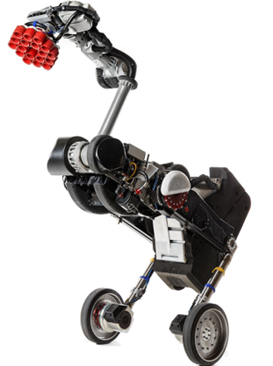
\includegraphics[width=0.5\textwidth]{figures/boston_handle.png}
  \caption{Boston Dynamics公司的轮腿式机器人Handle}
  \label{fig:boston-dynamics-handle}
\end{figure}

苏黎世联邦理工（ETH Zurich）的学生团队Victor Klemm 等人于2018 年9 月研制出了名为Ascento 的双轮跳跃机器人，[13]该机器人主要用于室内巡检，平整地面用轮子快速移动，并通过跳跃来越障。机械结构方面Ascento腿部采用四连杆机构，使整车结构紧凑。Ascento 通过线性二次调节器 (LQR)实现机器人的平衡和运动控制。对于跳跃和坠落恢复的机动过程，则使用带有反馈跟踪的顺序前馈控制器。跌倒恢复的控制策略是该机器人的一大创新，总结了轮腿式双足机器人跌倒后可能会出现的四种稳定位姿，并提出收缩腿部、受控伸展、施加力矩三个恢复步骤。

\begin{figure}[H]
  \centering
  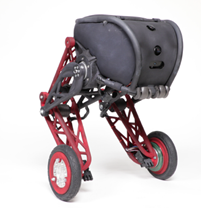
\includegraphics[width=0.4\textwidth]{figures/eth_1.png}
  \hspace{1cm}
  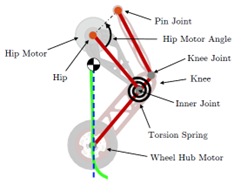
\includegraphics[width=0.4\textwidth]{figures/eth_2.png}
  \caption{Ascento机器人实物图（左）与简化图示（右）}
  \label{fig:eth-ascento}
\end{figure}


腾讯 AI Lab 及 Robotics X 实验室主任张正友博士在机器人行业顶会 ICRA 2021 做大会报告，分享了研发中的轮腿式机器人Ollie [14]，在视频中表现了双轮平衡、多模态移动、跳跃、360度空翻等运动能力。Ollie单腿采用并联机构，与身体形成五连杆结构，使整体具有结构简单、动态性能高、爆发力强的特点。机器人基本运动控制采用LQR控制器，此外为适应更多复杂场景，补充采用了IDA-PBC（interconnection and damping assignment- passivity-based control）。

\begin{figure}[H]
  \centering
  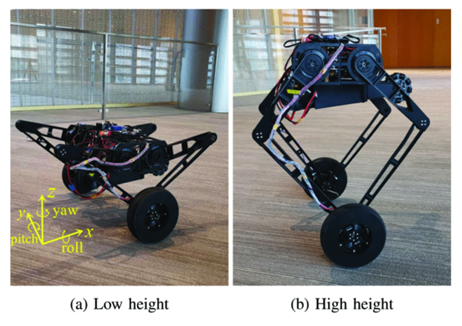
\includegraphics[width=0.5\textwidth]{figures/ollie.png}
  \caption{腾讯AI实验室研发的轮腿式机器人Ollie}
  \label{fig:tencent-ollie}
\end{figure}

\subsection{路径规划算法方案：基于深度强化学习的路径规划算法}

Tai et al.[15]提出了一种基于CNN的DRL模型，该模型以原始RGB-D图像为输入，移动机器人的控制命令为输出。CNN网络的初始权值来自于他们之前工作[13]中训练的参数。但是，由于奖励函数的设计没有涉及鼓励探索的机制，因此该模型只能在简单的走廊环境中实现避障。Jiang等人[17]提出了一种基于启发式制导和避障知识的DQN算法，在路径规划的训练效率和环境适应性方面取得了一定的效果。然而，由于启发式知识限制了DRL智能体的探索能力，规划的路径在路径长度和平滑度方面并不令人满意。[18] Niroui等人研究了一种将DRL与传统的基于边界的方法相结合的勘探模型。DRL模型输出边界点的权重参数，然后根据预定义的代价函数计算出代价最低的边界点。Chen等人[19]提出了一种基于DRL的探索方法，该方法以局部网格图为状态空间，动作空间为随机集合。Zhu等人[20]提出了一种分层DRL网络框架，其中低层DRL策略使机器人在向目标位置移动的同时与障碍物保持安全距离，高层DRL策略作为补充，进一步提高路径规划的安全性。同时，通过选择子目标节点减少状态空间，避免稀疏奖励，该方法在采样效率和迁移能力上都取得了出色的表现。
% <<< END INPUT chapters/07_intro.tex
% >>> BEGIN INPUT chapters/08_model.tex
\chapter{电缆机器人结构及动力学建模}\label{chap:model}

电缆机器人最终采取串联五连杆轮腿构型。为了实现对电缆机器人运动学和动力学的分析与控制，首先需要建立其结构模型和动力学模型。本章介绍电缆机器人的建模方法，包括坐标系定义、运动学分析和动力学推导。

% 设置视角: 
\tdplotsetmaincoords{70}{50} 
\begin{tikzpicture}[tdplot_main_coords, font=\footnotesize, >=latex]

% 1. 机器人坐标系 (在地面) 
% X: 右下, Y: 右上, Z: 上
\draw[->, thick, red] (0,0,0) -- (1.5,0,0);
\node[red] at (1.8, -0.4, 0) {机器人系}; 
\draw[->, thick, green] (0,0,0) -- (0,1.5,0);
\draw[->, thick, blue] (0,0,0) -- (0,0,1.5);

% 地平面辅助线
\draw[gray!50, dashed] (-1.5,-2,0) -- (3.5,-2,0) -- (3.5,2,0) -- (-1.5,2,0) -- cycle;

% 2. 轮子中心 (左右轮)
\coordinate (WL) at (0, 0.8, 0.4);
\coordinate (WR) at (0, -0.8, 0.4);

% 轮子 (在 Y-Z 平面内绘制，确保与地面相切)
\begin{scope}[canvas is yz plane at x=0]
    % 左轮：圆心 (y,z)=(0.8,0.4)，半径 0.4，最低点刚好接触 z=0
    \draw[thick, fill=white] (0.8, 0.4) circle (0.4);
    % 右轮：圆心 (y,z)=(-0.8,0.4)，半径 0.4，最低点刚好接触 z=0
    \draw[thick, fill=white] (-0.8, 0.4) circle (0.4);
\end{scope}

% 轮子转角指示 (简化显示)
\node at (0.3, 0.8, 0.8) {$\theta_{wl}$};
\node at (0.3, -0.8, 0.8) {$\theta_{wr}$};

% 3. 腿
\coordinate (BodyCenter) at (1.5, 0, 3.2);
\coordinate (HL) at (1.5, 0.8, 3.2);
\coordinate (HR) at (1.5, -0.8, 3.2);

\draw[thick] (WL) -- (HL);
\draw[thick] (WR) -- (HR);

% 左腿倾斜角 theta_ll
\draw[dashed, thin] (WL) -- ($(WL)+(0,0,2.5)$);
\draw[->, thin] ($(WL)+(0,0,1.5)$) arc[start angle=90, end angle=55, radius=1.5];
\node at ($(WL)+(0.4,0,1.8)$) {$\theta_{ll}$};

% 右腿倾斜角 theta_lr
\draw[dashed, thin] (WR) -- ($(WR)+(0,0,2.5)$);
\draw[->, thin] ($(WR)+(0,0,1.8)$) arc[start angle=90, end angle=55, radius=1.8];
\node at ($(WR)+(0.6,0,2.1)$) {$\theta_{lr}$};

% 4. 机体 (Base)
\begin{scope}[shift={(BodyCenter)}]
% 长方体
\draw[thick, fill=white, fill opacity=0.8] (-0.8,-1.2,-0.6) -- (1.2,-1.2,-0.6) -- (1.2,1.2,-0.6) -- (-0.8,1.2,-0.6) -- cycle; % 底面
\draw[thick] (-0.8,-1.2,-0.6) -- (-0.8,-1.2,0.6);
\draw[thick] (1.2,-1.2,-0.6) -- (1.2,-1.2,0.6);
\draw[thick] (1.2,1.2,-0.6) -- (1.2,1.2,0.6);
\draw[thick] (-0.8,1.2,-0.6) -- (-0.8,1.2,0.6);
\draw[thick, fill=white, fill opacity=0.8] (-0.8,-1.2,0.6) -- (1.2,-1.2,0.6) -- (1.2,1.2,0.6) -- (-0.8,1.2,0.6) -- cycle; % 顶面

% Base 坐标系
\draw[->, thick, red] (0,0,0) -- (2.5,0,0) node[anchor=north west]{机体系}; 
% \draw[->, thick] (2.8, -0.6, 0) -- (3.3, -1.0, 0) node[anchor=west]{$S$}; % 附加箭头S
\draw[->, thick, green] (0,0,0) -- (0,2.0,0);
\draw[->, thick, blue] (0,0,0) -- (0,0,2.5);

% theta_b 绕机体系红色轴（x轴）转动的示意弧线
\begin{scope}[canvas is yz plane at x=0]
    \draw[->, thick] (0, 1.0) arc[start angle=90, end angle=25, radius=1.0];
    \node at (0.55, 1.25) {$\theta_b$};
\end{scope}

% phi 绕 Z 轴偏航角弧线
\draw[->, thick] (0.2, 0, 2.3) arc[start angle=0, end angle=180, x radius=0.4, y radius=0.15];
\node at (0.4, 0.4, 2.5) {$\phi$};
\end{scope}

% 5. 'A' 视角指示
% \draw[->, thick, font=\LARGE] (-1.0, 3.0, 1.0) -- (0, 2.0, 1.0);
% \node at (-1.3, 3.2, 1.0) {$A$};

\end{tikzpicture}

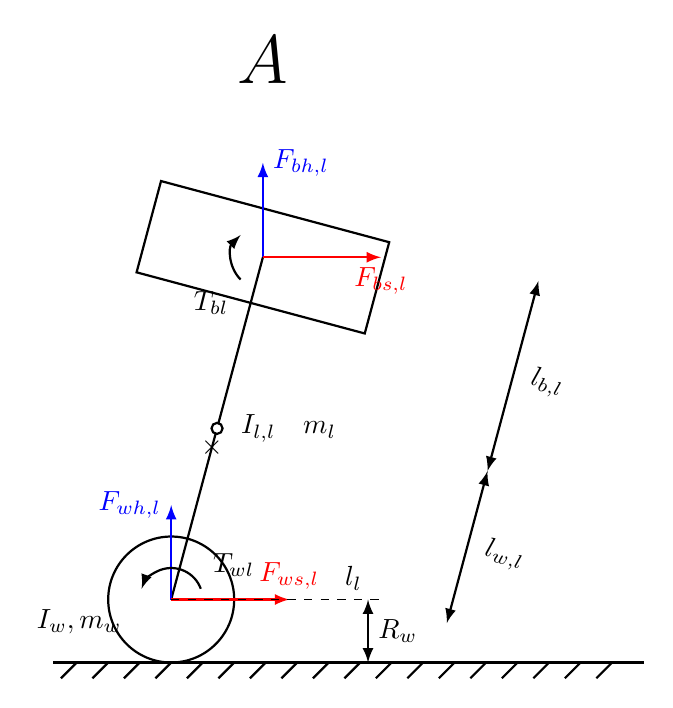
\begin{tikzpicture}[>=latex, line width=0.8pt]

    % --- 参数定义 ---
    \def\angle{75} % 腿部的倾斜角度
    \def\Rw{0.8}   % 轮子半径
    \def\Lw{2.0}   % 腿下半部分长度
    \def\Lb{2.5}   % 腿上半部分长度
    \def\rectW{3.0} % 身体矩形宽度
    \def\rectH{1.2} % 身体矩形高度

    % 坐标计算
    \coordinate (WheelCenter) at (0, \Rw);
    \coordinate (LegMid) at ($(WheelCenter) + (\angle:\Lw)$);
    \coordinate (BodyCenter) at ($(WheelCenter) + (\angle:\Lw+\Lb)$);

    % --- 绘制地面 ---
    \draw[thick] (-1.5, 0) -- (6, 0);
    \foreach \x in {-1.2,-0.8,...,5.8}
        \draw (\x, 0) -- (\x-0.2, -0.2);

    % --- 绘制轮子 ---
    \draw (WheelCenter) circle (\Rw);
    \node[anchor=north east] at ($(WheelCenter) + (-0.5, 0)$){$I_w, m_w$};

    % --- 绘制腿部 ---
    \draw (WheelCenter) -- (BodyCenter);
    % 腿部中点标记和标签 (修正了African拼写错误并正确放置标签)
    \filldraw[fill=white] ($(WheelCenter)!0.5!(BodyCenter)$ ) circle (2pt) node[right=5pt] {$I_{l,l} \quad m_l$};
    % 腿部分段标记 (叉号)
    \node at (LegMid) {$\times$};

    % --- 绘制身体 (倾斜矩形) ---
    \begin{scope}[shift={(BodyCenter)}, rotate={\angle-90}]
        \draw ( (-\rectW/2, -\rectH/2) rectangle (\rectW/2, \rectH/2);
    \end{scope}

    % --- 绘制力与力矩 (轮子处) ---
    % 垂直力 (蓝色)
    \draw[->, blue, thick] (WheelCenter) -- ++(0, 1.2) node[left] {$F_{wh,l}$};
    % 水平力 (红色)
    \draw[->, red, thick] (WheelCenter) -- ++(1.5, 0) node[above] {$F_{ws,l}$};
    
    % **修正后**的旋转力矩 T_{wl} (匹配原图，短逆时针弧)
    % 从右上方 (20:0.4) 逆时针画到左上方 (160:0.4)
    \draw[->] ($(WheelCenter) + (20:0.4)$) node[above right=1pt] {$T_{wl}$} arc[start angle=20, end angle=160, radius=0.4];

    % --- 绘制力与力矩 (身体处) ---
    % 垂直力 (蓝色)
    \draw[->, blue, thick] (BodyCenter) -- ++(0, 1.2) node[right] {$F_{bh,l}$};
    % 水平力 (红色)
    \draw[->, red, thick] (BodyCenter) -- ++(1.5, 0) node[below] {$F_{bs,l}$};
    
    \draw[->] ($(BodyCenter) + (225:0.4)$) node[below left=1pt] {$T_{bl}$} arc[start angle=225, delta angle=-90, radius=0.4];

    % --- 尺寸标注 ---
    % Rw 标注
    \draw[<->] (2.5, 0) -- (2.5, \Rw) node[midway, right] {$R_w$};
    \draw[thin, dashed] (WheelCenter) -- (2.7, \Rw);

    % 长度标注 (平行于腿部)
    \begin{scope}[shift={(3.5, 0.5)}, rotate=\angle]
        \draw[<->] (0, 0) -- (\Lw, 0) node[midway, right=3pt, rotate=\angle-90] {$l_{w,l}$};
        \draw[<->] (\Lw, 0) -- (\Lw+\Lb, 0) node[midway, right=3pt, rotate=\angle-90] {$l_{b,l}$};
        \node[right=20pt] at (0, 2.2) {$l_l$};
    \end{scope}

    % 顶部字母 A
    \node[font=\Huge] at ($(BodyCenter) + (0, 2.5)$) {$A$};

\end{tikzpicture}

\section{变量定义}

\renewcommand{\arraystretch}{1.3}
\begin{longtable}{>{\centering\arraybackslash}p{0.28\textwidth} >{\centering\arraybackslash}p{0.48\textwidth} >{\centering\arraybackslash}p{0.20\textwidth}}
    \caption{变量定义}\label{tab:variable_definition}\\
    \toprule
    \textbf{参数} & \textbf{含义} & \textbf{说明} \\
    \midrule
    \endfirsthead

    \multicolumn{3}{c}{\tablename\ \thetable\ 变量定义（续）}\\
    \toprule
    \textbf{参数} & \textbf{含义} & \textbf{说明} \\
    \midrule
    \endhead

    \midrule
    \multicolumn{3}{r}{续下页}\\
    \endfoot

    \bottomrule
    \endlastfoot

    $\theta_{w,i}$ $(i=l,r)$ & 驱动轮转角 & 自然坐标系法向 \\
    $\theta_{l,i}$ $(i=l,r)$ & 腿倾斜角 & 自然坐标系法向 \\
    $\theta_b$ & 机体倾斜角 & 自然坐标系法向 \\
    $\phi$ & 偏航角 &  \\
    $s$ & 自然坐标系下机器人水平方向移动距离 &  \\
    $s_b$ & 自然坐标系下机体质心水平方向移动距离 &  \\
    $h_b$ & 自然坐标系下机体质心竖直方向移动距离 &  \\
    $s_{l,i}$ $(i=l,r)$ & 自然坐标系下腿部质心水平方向移动距离 &  \\
    $h_{l,i}$ $(i=l,r)$ & 自然坐标系下腿部质心竖直方向移动距离 &  \\
    $T_{w,i}$ $(i=l,r)$ & 驱动轮转矩 & 腿-轮 \\
    $T_{b,i}$ $(i=l,r)$ & 腿部转矩 & 机体-腿 \\
    $f_i$ $(i=l,r)$ & 地面对驱动轮摩擦力 &  \\
    $F_{ws,i}$ $(i=l,r)$ & 驱动轮对腿水平方向作用力 &  \\
    $F_{wh,i}$ $(i=l,r)$ & 驱动轮对腿竖直方向作用力 &  \\
    $F_{bs,i}$ $(i=l,r)$ & 腿对机体水平方向作用力 &  \\
    $F_{bh,i}$ $(i=l,r)$ & 腿对机体竖直方向作用力 &  \\
    $R_w$ & 驱动轮半径 &  \\
    $R_l$ & 驱动轮轮距/2 &  \\
    $l_i$ $(i=l,r)$ & 腿长 &  \\
    $l_{w,i}$ $(i=l,r)$ & 驱动轮到腿部质心距离 &  \\
    $l_{b,i}$ $(i=l,r)$ & 驱动轮到腿部质心距离 &  \\
    $l_c$ & 机体质心到腿部关节距离 &  \\
    $m_w$ & 驱动轮质量 &  \\
    $m_l$ & 腿部质量 &  \\
    $m_b$ & 机体质量 &  \\
    $I_w$ & 驱动轮转动惯量（自然坐标系法向） &  \\
    $I_{l,i}$ $(i=l,r)$ & 腿部转动惯量（自然坐标系法向） &  \\
    $I_b$ & 机体转动惯量（自然坐标系法向） &  \\
    $I_z$ & 机器人$z$轴转动惯量 &  \\
\end{longtable}

*1：实际机器人腿部为五连杆机构，腿长可变，长度由腿部控制器控制，且质心位置、转动惯量均随腿长变化。\\
*2：绕z轴的转动惯量简化为常量。

\section{运动学模型}

根据变量、参数定义和几何关系得到系统的运动学方程，进而解得各变量的表达式

\begin{equation}
s = \frac{R_w}{2}(\theta_{w,l} + \theta_{w,r}) 
\label{eq:s}
\end{equation}

\begin{equation}
h_b = \frac{l_l}{2}\cos\theta_{l,l} + \frac{l_r}{2}\cos\theta_{l,r} 
\label{eq:h_b}
\end{equation}

\begin{equation}
s_{l,i} = R_w\theta_{w,i} + l_{w,i}\sin\theta_{l,i}
\label{eq:s_li}
\end{equation}

\begin{equation}
h_{l,i} = h_b - l_{b,i}\cos\theta_{l,i} 
\label{eq:h_li}
\end{equation}

\begin{equation}
R_w\theta_{w,l} = s_b - R_l\phi - l_l\sin\theta_{l,l} 
\label{eq:theta_wl}
\end{equation}

\begin{equation}
R_w\theta_{w,r} = s_b + R_l\phi - l_r\sin\theta_{l,r}
\label{eq:theta_wr}
\end{equation}

联立式 \ref{eq:theta_wl} 和 \ref{eq:theta_wr} 可解得 $s_b$ 和 $\phi$ 的表达式：

\begin{equation}
\phi = \frac{R_w}{2R_l}(-\theta_{w,l} + \theta_{w,r}) - \frac{l_l}{2R_l}\sin\theta_{l,l} + \frac{l_r}{2R_l}\sin\theta_{l,r} 
\label{eq:phi}
\end{equation}

\begin{equation}
s_b = \frac{R_w}{2}(\theta_{w,l} + \theta_{w,r}) + \frac{l_l}{2}\sin\theta_{l,l} + \frac{l_r}{2}\sin\theta_{l,r} 
\label{eq:s_b}
\end{equation}

式 \ref{eq:s}、\ref{eq:h_b}、\ref{eq:s_li}、\ref{eq:h_li}、\ref{eq:phi}、\ref{eq:s_b} 对时间分别求一/二阶导

\begin{equation}
\dot{s} = \frac{R_w}{2}(\dot{\theta}_{w,l} + \dot{\theta}_{w,r}) 
\label{eq:ds}
\end{equation}

\begin{equation}
\ddot{s} = \frac{R_w}{2}(\ddot{\theta}_{w,l} + \ddot{\theta}_{w,r}) 
\label{eq:dds}
\end{equation}

\begin{equation}
\dot{\phi} = \frac{R_w}{2R_l}(-\dot{\theta}_{w,l} + \dot{\theta}_{w,r}) - \frac{l_l}{2R_l}\cos\theta_{l,l}\dot{\theta}_{l,l} + \frac{l_r}{2R_l}\cos\theta_{l,r}\dot{\theta}_{l,r} 
\end{equation}

\begin{equation}
\ddot{\phi} = \frac{R_w}{2R_l}(-\ddot{\theta}_{w,l} + \ddot{\theta}_{w,r}) - \frac{l_l}{2R_l}\cos\theta_{l,l}\ddot{\theta}_{l,l} + \frac{l_r}{2R_l}\cos\theta_{l,r}\ddot{\theta}_{l,r} + \frac{l_l}{2R_l}\sin\theta_{l,l}\dot{\theta}_{l,l}^2 - \frac{l_r}{2R_l}\sin\theta_{l,r}\dot{\theta}_{l,r}^2 
\end{equation}

\begin{equation}
\dot{s}_b = \frac{R_w}{2}(\dot{\theta}_{w,l} + \dot{\theta}_{w,r}) + \frac{l_l}{2}\cos\theta_{l,l}\dot{\theta}_{l,l} + \frac{l_r}{2}\cos\theta_{l,r}\dot{\theta}_{l,r} 
\end{equation}

\begin{equation}
\ddot{s}_b = \frac{R_w}{2}(\ddot{\theta}_{w,l} + \ddot{\theta}_{w,r}) + \frac{l_l}{2}\cos\theta_{l,l}\ddot{\theta}_{l,l} + \frac{l_r}{2}\cos\theta_{l,r}\ddot{\theta}_{l,r} - \frac{l_l}{2}\sin\theta_{l,l}\dot{\theta}_{l,l}^2 - \frac{l_r}{2}\sin\theta_{l,r}\dot{\theta}_{l,r}^2 
\end{equation}

\begin{equation}
\dot{h}_b = -\frac{l_l}{2}\sin\theta_{l,l}\dot{\theta}_{l,l} - \frac{l_r}{2}\sin\theta_{l,r}\dot{\theta}_{l,r} 
\end{equation}

\begin{equation}
\ddot{h}_b = -\frac{l_l}{2}\sin\theta_{l,l}\ddot{\theta}_{l,l} - \frac{l_r}{2}\sin\theta_{l,r}\ddot{\theta}_{l,r} - \frac{l_l}{2}\cos\theta_{l,l}\dot{\theta}_{l,l}^2 - \frac{l_r}{2}\cos\theta_{l,r}\dot{\theta}_{l,r}^2 
\end{equation}

\begin{equation}
\dot{s}_{l,i} = R_w\dot{\theta}_{w,i} + l_{w,i}\cos\theta_{l,i}\dot{\theta}_{l,i} 
\end{equation}

\begin{equation}
\ddot{s}_{l,i} = R_w\ddot{\theta}_{w,i} + l_{w,i}\cos\theta_{l,i}\ddot{\theta}_{l,i} - l_{w,i}\sin\theta_{l,i}\dot{\theta}_{l,i}^2 
\end{equation}

\begin{equation}
\dot{h}_{l,i} = \dot{h}_b + l_{b,i}\sin\theta_{l,i}\dot{\theta}_{l,i} 
\end{equation}

\begin{equation}
\ddot{h}_{l,i} = \ddot{h}_b + l_{b,i}\sin\theta_{l,i}\ddot{\theta}_{l,i} + l_{b,i}\cos\theta_{l,i}\dot{\theta}_{l,i}^2 
\end{equation}

\section{动力学模型}

本节基于拉格朗日法建立系统动力学方程，并给出关节力矩与广义坐标之间的关系。

使用牛顿欧拉法建立系统的动力学方程

对于左右驱动轮（$i = l, r$）
\begin{equation}
m_w R_w \ddot{\theta}_{w,i} = f_i - F_{ws,i} 
\end{equation}

\begin{equation}
I_w \ddot{\theta}_{w,i} = T_{w,i} - f_i R_w
\end{equation}

对于左右腿（$i = l, r$）
\begin{equation}
m_l \ddot{s}_{l,i} = F_{ws,i} - F_{bs,i} 
\end{equation}

\begin{equation}
m_l \ddot{h}_{l,i} = F_{wh,i} - F_{bh,i} - m_l g 
\end{equation}

\begin{equation}
I_{l,i} \ddot{\theta}_{l,i} = (F_{wh,i} l_{w,i} + F_{bh,i} l_{b,i}) \sin\theta_{l,i} - (F_{ws,i} l_{w,i} + F_{bs,i} l_{b,i}) \cos\theta_{l,i} - T_{w,i} + T_{b,i} 
\end{equation}

对于机体
\begin{equation}
m_b \ddot{s}_b = F_{bs,l} + F_{bs,r} 
\end{equation}

\begin{equation}
m_b \ddot{h}_b = F_{bh,l} + F_{bh,r} - m_b g 
\end{equation}

\begin{equation}
I_b \ddot{\theta}_b = -(T_{b,l} + T_{b,r}) - (F_{bs,l} + F_{bs,r}) l_c \cos\theta_b + (F_{bh,l} + F_{bh,r}) l_c \sin\theta_b
\end{equation}

机器人整体偏航（yaw）方向旋转
\begin{equation}
I_z \ddot{\phi} = (-f_l + f_r) R_l 
\end{equation}

左右腿支持力相等
\begin{equation}
F_{wh,l} = F_{wh,r} 
\end{equation}

本节建立轮腿机构的位置与速度映射关系，为后续控制器设计提供基础。

\section{方程化简求解}
由于运动学与动力学方程繁多且复杂，直接化简求解较为困难，故采用python脚本进行化简求解。

化简得
% 方程 (3.13)
\begin{equation}
\resizebox{0.98\linewidth}{!}{$
\frac{-R_w \left[ \ddot{\theta}_{l,l} (l_{bl} m_b + l_{wl} m_b + 2l_{wl} m_l) + \ddot{\theta}_{l,r} (l_{br} m_b + l_{wr} m_b + 2l_{wr} m_l) \right] + 2T_{lwl} + 2T_{lwr} - (\ddot{\theta}_{wl} + \ddot{\theta}_{wr}) \left[ 2I_w + R_w^2 (m_b + 2m_l + 2m_w) \right]}{2R_w} = 0
$}
\label{eq:x_y_move}
\end{equation}

% 方程 (3.14)
\begin{equation}
\resizebox{0.98\linewidth}{!}{$
\frac{R_w \left( I_b \ddot{\theta}_b + T_{bll} + T_{blr} + \ddot{\theta}_{l,l} l_c l_{wl} m_l + \ddot{\theta}_{l,r} l_c l_{wr} m_l - g l_c m_b \theta_b \right) - (T_{lwl} + T_{lwr}) l_c + (\ddot{\theta}_{wl} + \ddot{\theta}_{wr}) l_c \left[ I_w + R_w^2 (m_l + m_w) \right]}{R_w} = 0
$}
\label{eq:pitch_move}
\end{equation}

% 方程 (3.15)
\begin{equation}
\resizebox{0.98\linewidth}{!}{$
\frac{I_z R_w \left[ -\ddot{\theta}_{l,l}(l_{bl} + l_{wl}) + \ddot{\theta}_{l,r}(l_{br} + l_{wr}) \right] + 2R_l^2 (T_{lwl} - T_{lwr}) + (\ddot{\theta}_{wr} - \ddot{\theta}_{wl}) (2I_w R_l^2 + I_z R_w^2)}{2R_l R_w} = 0
$}
\label{eq:yaw_move}
\end{equation}

这三个方程分别从系统的平动、俯仰和偏航三个自由度出发，揭示了轮足机器人在复杂动力学耦合下的运动规律，为后续的控制器设计提供了理论基础。以下将对每个方程的物理意义进行详细解析。

\subsection{纵向平移运动学平衡方程(方程\ref{eq:x_y_move})}

本节构建了轮足机器人在纵向（$x$轴方向）的平移加速度与驱动力矩之间的映射关系。根据达朗贝尔原理（D'Alembert's Principle），系统在前进方向上的广义力平衡方程可表述为：$$\sum F_x = M_{eq} \cdot a_x + F_{coupling}$$

等效质量与转动惯量折算：方程 (3.13) 中的系数项 $2I_w + R_{w}^{2}(m_b + 2m_l + 2m_w)$ 反映了系统的等效平移惯量。其中不仅包含机体、腿部及轮组的静质量，还通过轮径 $R_w$ 将驱动轮的转动惯量 $I_w$ 折算至线加速度维度。这体现了系统在平移过程中，能量在平动动能与转动动能之间的耦合分布。

腿部运动耦合：项 $\ddot{\theta}_{l,l}$ 与 $\ddot{\theta}_{l,r}$ 的系数代表了腿部摆动产生的惯性力对底盘平移的影响。当腿部角度发生剧烈变化时，其质心位置的水平加速度会通过关节反作用力直接作用于底盘。

驱动输入：$2T_{lw}$ 为系统的主动控制量，代表左右电机在接触点产生的等效牵引力。

\subsection{俯仰轴动力学平衡方程(方程\ref{eq:pitch_move})}

俯仰方向的稳定性是轮足机器人平衡控制的核心，该方程本质上是一个线性化后的倒立摆模型。

姿态动力学项：$I_b \ddot{\theta}_b$ 描述了机体绕其质心的旋转惯性。

不稳定重力矩：$-g l_c m_b \theta_b$ 项具有正反馈特性，代表了重力在机体偏离平衡位置时产生的倾覆力矩。在线性化分析中，该项决定了系统的开环不稳定性，是控制器设计时需要补偿的主要干扰。

位移-姿态耦合项：$\ddot{\theta}_{w}$ 项的引入体现了“加速度诱导力矩”效应。当底盘产生水平加速度时，由于机体质心与轮轴存在高度差 $l_c$，会在俯仰方向产生显著的惯性耦合力矩。这也是实现“以位移保平衡”控制策略的物理基础。

\subsection{偏航轴动力学平衡方程(方程\ref{eq:yaw_move})}

偏航（Yaw）方程描述了机器人朝向姿态角的演化逻辑，主要涉及空间动力学的角动量守恒与差速驱动原理。

偏航惯量矩阵：系数 $2I_w R_{l}^{2} + I_z R_{w}^{2}$ 定义了系统绕几何中心转动的总等效惯量。它综合考虑了机体绕 $Z$ 轴的转动惯量 $I_z$ 以及左右轮组在差速转动时的旋转动量。

差速驱动逻辑：该方程的核心输入为 $(T_{lw,l} - T_{lw,r})$。通过建立电机力矩差与偏航加速度 $\ddot{\psi}$ 的线性关系，将复杂的地面摩擦力约束简化为由力矩差驱动的二阶系统，简化了偏航控制器的解耦设计。

非对称干扰补偿：腿部伸缩或摆动加速度的非对称性（$\ddot{\theta}_{l,r} - \ddot{\theta}_{l,l}$）会导致偏航干扰。方程中对应的系数项为控制算法提供了前馈补偿的理论依据，以确保机器人在高速直线行驶中不发生偏离。

\section{五连杆运动学模型与VMC}

\subsection{五连杆运动学解算}

\begin{figure}[H]
  \centering
  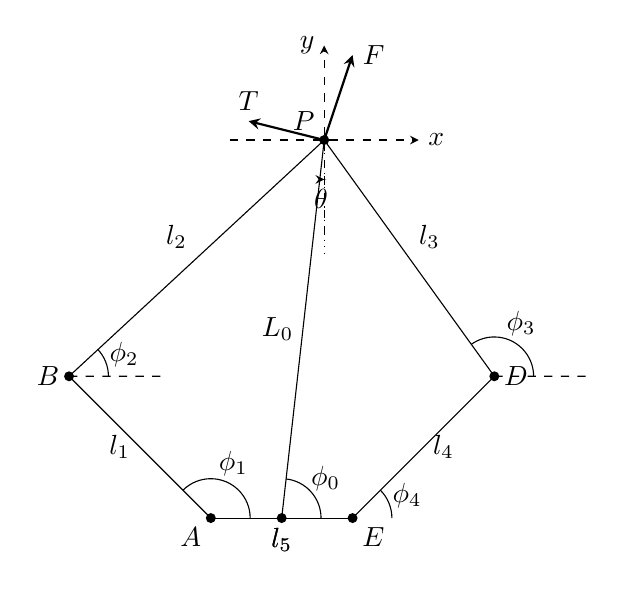
\begin{tikzpicture}[scale=1.2, >=stealth]
    
    % --- 定义关键点坐标 (基于原图比例估算) ---
    \coordinate (A) at (1, 0);
    \coordinate (E) at (2.5, 0);
    \coordinate (B) at (-0.5, 1.5);
    \coordinate (D) at (4, 1.5);
    \coordinate (P) at (2.2, 4); % 原 C 点，已重命名为 P
    \coordinate (L5_mid) at (1.75, 0); % L0 连接在 l5 上的点
    
    % --- 绘制杆件和地面 ---
    \draw (A) -- (E) node[midway, below] {$l_5$}; % 地面
    \draw (A) -- (B) node[midway, left] {$l_1$};
    \draw (B) -- (P) node[midway, above left] {$l_2$};
    \draw (P) -- (D) node[midway, above right] {$l_3$};
    \draw (D) -- (E) node[midway, right] {$l_4$};
    \draw (L5_mid) -- (P) node[midway, left] {$L_0$};
    
    % --- 绘制点和标签 ---
    \fill (A) circle (1.5pt) node[below left] {$A$};
    \fill (E) circle (1.5pt) node[below right] {$E$};
    \fill (B) circle (1.5pt) node[left] {$B$};
    \fill (D) circle (1.5pt) node[right] {$D$};
    \fill (P) circle (1.5pt) node[above left] {$P$}; % 已改为 P
    \fill (L5_mid) circle (1.5pt) node[below] {$l_5$ }; % 这里标记mid点为l5也可
    
    % --- 在 P 点 (原C点) 绘制坐标系 ---
    \begin{scope}[shift={(P)}]
      \draw[dashed, ->] (-1, 0) -- (1, 0) node[right] {$x$};
      \draw[dashed, ->] (0, -1) -- (0, 1) node[left] {$y$};
      
      % 绘制力向量 T 和 F
      \draw[thick, ->] (0,0) -- (-0.8, 0.2) node[above] {$T$};
      \draw[thick, ->] (0,0) -- (0.3, 0.9) node[right] {$F$};
      
      % --- 新增：标注 L0 与 y 轴夹角 \theta ---
      % 计算 L0 (P 到 L5_mid) 的反向角度
      \coordinate (L0_dir) at ($ (L5_mid) - (P) $);
      \coordinate (O_node) at (0,0);
      \coordinate (Y_neg) at (0,-1.2);
      % 绘制 y 轴负方向和夹角
      \draw[dotted] (O_node) -- (Y_neg);
      \pic [draw, ->, "$\theta$", angle eccentricity=1.5] {angle = L0_dir--O_node--Y_neg};
      % 注意：需要 \usetikzlibrary{quotes,angles}
    \end{scope}
    
    % --- 标注角度 \phi ---
    % 定义水平基准方向
    \coordinate (H_A) at ($ (A) + (1, 0) $);
    \coordinate (H_B) at ($ (B) + (1, 0) $);
    \coordinate (H_E) at ($ (E) + (1, 0) $);
    \coordinate (H_D) at ($ (D) + (1, 0) $);
    \coordinate (H_L) at ($ (L5_mid) + (1, 0) $);

    % 绘制 B 和 D 点向右的水平虚线射线
    \draw[dashed] (B) -- (H_B);
    \draw[dashed] (D) -- (H_D);

    \pic [draw, "$\phi_1$", angle eccentricity=1.5] {angle = H_A--A--B};
    \pic [draw, "$\phi_2$", angle eccentricity=1.5] {angle = H_B--B--P}; % 这里phi2角度需按图示调整
    \pic [draw, "$\phi_4$", angle eccentricity=1.5] {angle = H_E--E--D}; % \phi_4 为角 DEA 劣弧
    \pic [draw, "$\phi_3$", angle eccentricity=1.5] {angle = H_D--D--P}; % 修正为 H_D--D--E
    \pic [draw, "$\phi_0$", angle eccentricity=1.5] {angle = H_L--L5_mid--P};

  \end{tikzpicture}
  \caption{五杆机构结构示意图与参数定义}
  \label{fig:linkage-analysis}
\end{figure}

\begin{table}[H]
  \centering
  \caption{五连杆相关参数定义}\label{tab:five_bar_definition}
  \renewcommand{\arraystretch}{1.3}
  \begin{tabular}{llp{5cm}}
    \toprule
    \textbf{参数} & \textbf{含义} & \textbf{说明} \\
    \midrule
    $\phi_1$ & 前腿电机转动角度 & 通过前腿电机编码器读取 \\
    $\phi_4$ & 后腿电机转动角度 & 通过后腿电机编码器读取 \\
    $l_1$ & 前腿长度 & 五连杆机构的前侧主连杆长度 \\
    $l_2$ & 后腿长度 & 五连杆机构的后侧主连杆长度 \\
    $l_3$ & 对侧前腿长度 & 一般设计$l_3=l_1$ \\
    $l_4$ & 对侧后腿长度 & 一般设计$l_4=l_2$ \\
    $L_0$ & 等效虚拟腿长 & 由五连杆机构几何关系计算得到 \\
    $\varPhi_0$ & 虚拟腿摆角 & 虚拟腿相对机体的摆动角 \\
    $\theta$ & 虚拟腿倾角 &虚拟腿相对于地面的倾角\\
    \bottomrule
  \end{tabular}
\end{table}

五连杆机构参数定义如图~\ref{fig:linkage-analysis} 和表~\ref{tab:five_bar_definition} 所示，其中 A、E 为两个电机转动副，其角度 $\phi_1$、$\phi_4$ 可通过电机编码器测量得到；B、C、D 为连杆转动副，其角度 $\phi_2$、$\phi_3$由机构运动学关系确定。

设足端点为 $P(x_p, z_p)$，其位置可表示为
\begin{equation}
  \begin{aligned}
    x_p &= f_x(\phi_1,\phi_4,l_1,l_2)\\
    z_p &= f_z(\phi_1,\phi_4,l_1,l_2)
  \end{aligned}
\end{equation}

其中具体几何推导为：

通过五连杆左右两部分列写 $P$ 点坐标，可得到以下等式：
\begin{equation}
    \begin{cases}
        x_B + l_2 \cos \phi_2 = x_D + l_3 \cos \phi_3 \\
        y_B + l_2 \sin \phi_2 = y_D + l_3 \sin \phi_3
    \end{cases}
    \label{eq:kinematic_constraints}
\end{equation}

求解方程组可得到角度 $\phi_2$：
\begin{equation}
    \phi_2 = 2 \arctan \left( \frac{B_0 + \sqrt{A_0^2 + B_0^2 - C_0^2}}{A_0 + C_0} \right)
\end{equation}

其中：
\begin{equation}
    \begin{aligned}
        A_0 &= 2l_2(x_D - x_B) \\
        B_0 &= 2l_2(y_D - y_B) \\
        C_0 &= l_2^2 + l_{BD}^2 - l_3^2 \\
        l_{BD} &= \sqrt{(x_D - x_B)^2 + (y_D - y_B)^2}
    \end{aligned}
\end{equation}

通过角度 $\phi_2$ 即可解算出 $P$ 点直角坐标 $(x, y)$：
\begin{equation}
    \begin{cases}
        x_P = l_1 \cos \phi_1 + l_2 \cos \phi_2 \\
        y_P = l_1 \sin \phi_1 + l_2 \sin \phi_2
    \end{cases}
    \label{eq:x_c_coordination}
\end{equation}

进而得到极坐标 $(L_0, \phi_0)$：
\begin{equation}
    \begin{cases}
        L_0 = \sqrt{(x_C - l_5 / 2)^2 + y_C^2} \\
        \phi_0 = \arctan \dfrac{y_C}{x_C - l_5 / 2}
    \end{cases}
    \label{eq:l0_phi0}
\end{equation}

通过上述关系，可以将电机角度 $\phi_1$、$\phi_4$ 映射到足端位置 $P(x_p, z_p)$，实现对足端位置的控制。

\subsection{五连杆动态静力学}
\begin{figure}[H]
  \centering
  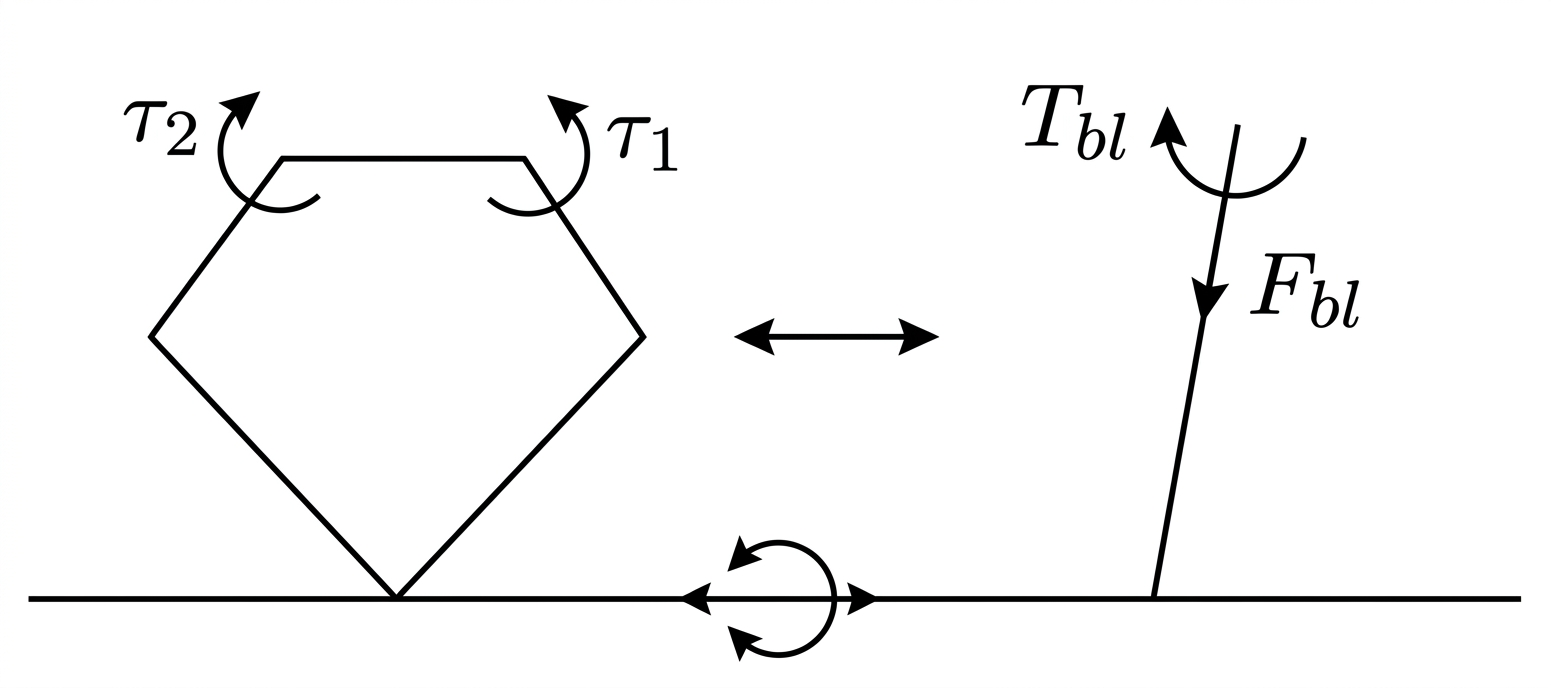
\includegraphics[width=0.5\textwidth]{figures/five_bar_kinetics.png}
  \caption{五连杆机构动态静力学分析}
  \label{fig:five-bar-kinetics}
\end{figure}

动态静力学记 $\gamma = [F_{bl} \quad T_{bl}]^T$，$\tau = [\tau_1 \quad \tau_2]^T$根据虚功原理可得：
\begin{equation}
    \tau = J^T \gamma \quad
    \label{eq:five-bar-kinetics}
\end{equation}

公式\ref{eq:five-bar-kinetics} 描述了足端力、力矩 $\gamma$ 与关节电机力矩 $\tau$ 之间的映射关系，$J^T$ 是雅可比矩阵的转置。由此可见，通过计算雅可比矩阵 $J$，可以将足端的期望力、力矩 $\gamma$ 转换为对应的关节电机力矩 $\tau$，实现对五连杆机构的动态控制。控制将简化为直接控制单根虚拟腿杆件。

\subsection{VMC与雅各比矩阵}
虚拟模型控制（Virtual Model Control，VMC）是一种直观且有效的运动学与动力学控制方法，广泛应用于足式和轮腿式机器人的平衡与运动控制中。其核心思想是在机器人内部或机器人与其所处环境（如机体中心与地面支撑点）之间，引入虚拟的机械元件（如虚拟弹簧、虚拟阻尼器等），以计算出使其实现期望运动或维持期望姿态所需的“虚拟力”。随后，借助机构的雅可比矩阵，将这组虚拟力映射为对应各个物理关节的期望输入力矩。

在本文设计的轮腿系统中，通常将复杂的五连杆结构等效为一根具备可变长度与角度的“虚拟腿”。通过在虚拟腿和机体的质心之间布置径向与切向的虚拟弹簧阻尼系统，并通过调节虚拟腿长 $L_0$ 与摆角 $\varPhi_0$ 的期望值，即可实现对电缆机器人机体的高度、支撑力以及俯仰姿态的平滑协调控制。为了将虚拟模型得到的端点控制力矩分配到实际的驱动电机上，需要进一步推导从关节空间到虚拟腿空间的雅各比矩阵映射关系。

VMC是一种直观控制方式，其关键是在每个需要控制的自由度上构造恰当的虚拟构件以产生合适的虚拟力。虚拟力不是实际执行机构的作用力或力矩，而是通过执行机构的作用经过机构转换而成。对于一些控制问题，我们可能需要将工作空间（Task Space）的力或力矩映射成关节空间（Joint Space）的关节力矩。

在该五连杆问题中，我们需要获得五连杆机构末端沿腿的推力 $F$ 与沿中心轴的力矩 $T_p$（分别对应极坐标 $L_0, \phi_0$）与 $A, E$ 两转动副的驱动电机力矩 $T_1, T_2$ 的映射关系。定义 $\boldsymbol{x} = [L_0 \quad \phi_0]^T, \boldsymbol{q} = [\phi_1 \quad \phi_4]^T$，对正运动学模型 $\boldsymbol{x} = f(\boldsymbol{q})$ 求全微分得：
\begin{equation}
    \begin{cases}
        \delta L_0 = \frac{\partial f_1}{\partial \phi_1} \delta \phi_1 + \frac{\partial f_1}{\partial \phi_4} \delta \phi_4 \\
        \delta \phi_0 = \frac{\partial f_2}{\partial \phi_1} \delta \phi_1 + \frac{\partial f_2}{\partial \phi_4} \delta \phi_4
    \end{cases}
    \label{eq:differential}
\end{equation}

即：
\begin{equation}
    \delta \boldsymbol{x} = 
    \begin{bmatrix}
        \frac{\partial f_1}{\partial \phi_1} & \frac{\partial f_1}{\partial \phi_4} \\
        \frac{\partial f_2}{\partial \phi_1} & \frac{\partial f_2}{\partial \phi_4}
    \end{bmatrix} \delta \boldsymbol{q}
\end{equation}

定义雅可比矩阵 $\boldsymbol{J}$ 为：
\begin{equation}
    \boldsymbol{J} = 
    \begin{bmatrix}
        \frac{\partial f_1}{\partial \phi_1} & \frac{\partial f_1}{\partial \phi_4} \\
        \frac{\partial f_2}{\partial \phi_1} & \frac{\partial f_2}{\partial \phi_4}
    \end{bmatrix}
    \label{eq:jacob_def}
\end{equation}

有：
\begin{equation}
    \delta \boldsymbol{x} = \boldsymbol{J} \delta \boldsymbol{q}
\end{equation}

即通过雅可比矩阵 $\boldsymbol{J}$ 将关节速度 $\dot{\boldsymbol{q}}$ 映射为五连杆姿态变化率 $\dot{\boldsymbol{x}}$。根据虚功原理，有：
\begin{equation}
    \boldsymbol{T}^T \delta \boldsymbol{q} + (-\boldsymbol{F})^T \delta \boldsymbol{x} = 0
\end{equation}

其中 $\boldsymbol{T} = [T_1 \quad T_2]^T, \boldsymbol{F} = [F \quad T_p]^T$。将式 $\delta \boldsymbol{x} = \boldsymbol{J} \delta \boldsymbol{q}$ 代入，有：
\begin{equation}
    \boldsymbol{T} = \boldsymbol{J}^T \boldsymbol{F}
\end{equation}

综上通过正运动学模型雅可比矩阵即可解算出关节电机输出力矩。

但对上文推导出的正运动学模型直接求取雅可比矩阵 $\boldsymbol{J}$ 并不是好办法，因为模型表达式中包含大量平方与三角函数及其嵌套运算，直接调用符号运算工具的求雅可比矩阵函数会得到极其复杂的结果，无法转移到嵌入式平台进行计算，故需要通过其他方法来计算。

根据式 \eqref{eq:jacob_def} 可知，雅可比矩阵 $\boldsymbol{J}$ 实际描述的是两坐标微分的线性映射关系，因此我们可以通过计算速度映射关系来得到雅可比矩阵。

对式 \eqref{eq:x_c_coordination} 求导可得：
\begin{equation}
    \begin{cases}
        \dot{x}_C = -l_1 \dot{\phi}_1 \sin \phi_1 - l_2 \dot{\phi}_2 \sin \phi_2 \\
        \dot{y}_C = l_1 \dot{\phi}_1 \cos \phi_1 + l_2 \dot{\phi}_2 \cos \phi_2
    \end{cases}
    \label{eq:vel_c}
\end{equation}

其中 $\dot{\phi}_1$ 可由电机编码器测得。对式 \eqref{eq:kinematic_constraints} 求导可计算 $\dot{\phi}_2$：
\begin{equation}
    \begin{cases}
        \dot{x}_B - l_2 \dot{\phi}_2 \sin \phi_2 = \dot{x}_D - l_3 \dot{\phi}_3 \sin \phi_3 \\
        \dot{y}_B + l_2 \dot{\phi}_2 \cos \phi_2 = \dot{y}_D + l_3 \dot{\phi}_3 \cos \phi_3
    \end{cases}
    \label{eq:vel_b_d}
\end{equation}

消去 $\dot{\phi}_3$ 求得 $\dot{\phi}_2$：
\begin{equation}
    \dot{\phi}_2 = \frac{(\dot{x}_D - \dot{x}_B) \cos \phi_3 + (\dot{y}_D - \dot{y}_B) \sin \phi_3}{l_2 \sin(\phi_3 - \phi_2)}
\end{equation}

其中：
\begin{equation}
    \begin{cases}
        \dot{x}_B = -l_2 \dot{\phi}_1 \sin \phi_1 \\
        \dot{y}_B = l_2 \dot{\phi}_1 \cos \phi_1 \\
        \dot{x}_D = -l_4 \dot{\phi}_4 \sin \phi_4 \\
        \dot{y}_D = l_4 \dot{\phi}_4 \cos \phi_4
    \end{cases}
\end{equation}

将 $\dot{\phi}_2$ 代入式 \eqref{eq:vel_c} 即可得到：
\begin{equation}
    \begin{cases}
        \dot{x}_C = -l_1 \dot{\phi}_1 \sin \phi_1 - l_2 \left( \frac{(\dot{x}_D - \dot{x}_B) \cos \phi_3 + (\dot{y}_D - \dot{y}_B) \sin \phi_3}{l_2 \sin(\phi_3 - \phi_2)} \right) \sin \phi_2 \\
        \dot{y}_C = l_1 \dot{\phi}_1 \cos \phi_1 + l_2 \left( \frac{(\dot{x}_D - \dot{x}_B) \cos \phi_3 + (\dot{y}_D - \dot{y}_B) \sin \phi_3}{l_2 \sin(\phi_3 - \phi_2)} \right) \cos \phi_2
    \end{cases}
\end{equation}

可以看到，通过这种方法计算的公式不再包含平方与三角函数嵌套运算，三角函数之间的加减乘除也可以利用两角和差公式进一步化简。

得：
\begin{equation}
    \begin{bmatrix}
        \dot{x}_C \\ \dot{y}_C
    \end{bmatrix} = 
    \begin{bmatrix}
        \frac{l_1 \sin(\phi_1 - \phi_2) \sin \phi_3}{\sin(\phi_2 - \phi_3)} & \frac{l_4 \sin(\phi_3 - \phi_4) \sin \phi_2}{\sin(\phi_2 - \phi_3)} \\
        -\frac{l_1 \sin(\phi_1 - \phi_2) \cos \phi_3}{\sin(\phi_2 - \phi_3)} & -\frac{l_4 \sin(\phi_3 - \phi_4) \cos \phi_2}{\sin(\phi_2 - \phi_3)}
    \end{bmatrix}
    \begin{bmatrix}
        \dot{\phi}_1 \\ \dot{\phi}_4
    \end{bmatrix}
    \label{eq:jacob_full}
\end{equation}

记作：
\begin{equation}
    \begin{bmatrix}
        \dot{x}_C \\ \dot{y}_C
    \end{bmatrix} = \boldsymbol{J}
    \begin{bmatrix}
        \dot{\phi}_1 \\ \dot{\phi}_4
    \end{bmatrix}
\end{equation}

根据上式，可得到关节力矩 $[T_1 \quad T_2]^T$ 与虚拟力 $[F_x \quad F_y]^T$ 的映射关系：
\begin{equation}
    \begin{bmatrix}
        T_1 \\ T_2
    \end{bmatrix} = \boldsymbol{J}^T
    \begin{bmatrix}
        F_x \\ F_y
    \end{bmatrix}
\end{equation}

利用旋转矩阵 $\boldsymbol{R}$ 将 $[F_x \quad F_y]^T$ 旋转至极坐标方向：
\begin{equation}
    \begin{bmatrix}
        F_x \\ F_y
    \end{bmatrix} = 
    \begin{bmatrix}
        \cos(\phi_0 - \pi/2) & -\sin(\phi_0 - \pi/2) \\
        \sin(\phi_0 - \pi/2) & \cos(\phi_0 - \pi/2)
    \end{bmatrix}
    \begin{bmatrix}
        F_c \\ F_t
    \end{bmatrix}
\end{equation}

其中 $F_t, F_c$ 分别是末端沿 $L_0$ 和垂直于 $L_0$ 的虚拟力，再利用变换矩阵 $\boldsymbol{M}$ 可映射至最终的虚拟力 $\boldsymbol{F} = [F \quad T_p]^T$：
\begin{equation}
    \begin{bmatrix}
        F_t \\ F_c
    \end{bmatrix} = 
    \begin{bmatrix}
        0 & -\frac{1}{L_0} \\
        1 & 0
    \end{bmatrix}
    \begin{bmatrix}
        F \\ T_p
    \end{bmatrix}
\end{equation}

将上述表达式依次代入 ~\ref{eq:kinematic_constraints} 得到最终的关节力矩与虚拟力映射关系：
\begin{equation}
    \begin{bmatrix}
        T_1 \\ T_2
    \end{bmatrix} = \boldsymbol{J}^T \boldsymbol{R} \boldsymbol{M}
    \begin{bmatrix}
        F \\ T_p
    \end{bmatrix}
\end{equation}

利用 MATLAB 进行上述计算：
\begin{lstlisting}[language=Matlab]
R = [cos(phi0-pi/2) -sin(phi0-pi/2);
     sin(phi0-pi/2)  cos(phi0-pi/2)];
M = [0 -1/L0;
     1  0];
T = simplify(J.'*R*M)
\end{lstlisting}

得到最终结果：
\begin{equation}
    \begin{bmatrix}
        T_1 \\ T_2
    \end{bmatrix} = 
    \begin{bmatrix}
        \frac{l_1 \sin(\phi_0 - \phi_3) \sin(\phi_1 - \phi_2)}{\sin(\phi_3 - \phi_2)} & \frac{l_1 \cos(\phi_0 - \phi_3) \sin(\phi_1 - \phi_2)}{L_0 \sin(\phi_3 - \phi_2)} \\
        \frac{l_4 \sin(\phi_0 - \phi_2) \sin(\phi_3 - \phi_4)}{\sin(\phi_3 - \phi_2)} & \frac{l_4 \cos(\phi_0 - \phi_2) \sin(\phi_3 - \phi_4)}{L_0 \sin(\phi_3 - \phi_2)}
    \end{bmatrix}
    \begin{bmatrix}
        F \\ T_p
    \end{bmatrix}
\end{equation}

\subsection{机器人具体结构参数设定}
由于后续需要继续进行动力学建模与控制器设计，因此需要对机器人结构参数进行具体设定。根据前文的设计方案，机器人采用串联五连杆轮腿构型，相关参数定义如表~\ref{tab:five_bar_definition} 所示。

\begin{table}[htbp]
  \centering
  \caption{机器人基本几何参数设定}\label{tab:geometry_params}
  \renewcommand{\arraystretch}{1.3}
  \begin{tabularx}{\textwidth}{>{\centering\arraybackslash}X >{\centering\arraybackslash}X >{\centering\arraybackslash}X}
    \toprule
    \textbf{参数} & \textbf{含义} & \textbf{数值} \\
    \midrule
    $R$ & 驱动轮半径 & 0.06m \\
    $R_l$ & 轮距的一半 & 0.2395m \\
    $l_c$ & 质心偏移 & 0.035m \\
    \bottomrule
  \end{tabularx}
\end{table}

\begin{table}[H]
  \centering
  \caption{机器人腿部参数设定}\label{tab:leg_params}
  \renewcommand{\arraystretch}{1.3}
  \begin{tabularx}{\textwidth}{>{\centering\arraybackslash}X >{\centering\arraybackslash}X >{\centering\arraybackslash}X}
    \toprule
    \textbf{参数} & \textbf{含义} & \textbf{数值} \\
    \midrule
    $R$ & 驱动轮半径 & 0.06m \\
    $m_w$ & 单个轮子质量 & 0.9kg \\
    $m_l$ & 单条腿质量 & 1.948kg \\
    $m_b$ & 身体质量 & 25.0kg \\
    $I_ll$ & 左腿转动惯量 &$0.03kg\cdot m^2$\\
    $I_lr$ & 右腿转动惯量 &$0.03kg\cdot m^2$\\
    \bottomrule
  \end{tabularx}
\end{table}
% <<< END INPUT chapters/08_model.tex
% >>> BEGIN INPUT chapters/09_control.tex
\chapter{电缆机器人的控制方案设计}\label{chap:control}

由\ref{chap:model}章，我们将整个机器人五连杆腿部结构进行几何分析解算，等效为一根虚拟连杆为虚拟腿，并计算了虚拟腿长、虚拟腿倾角等相关数据。经过虚拟腿的简化，整个机器人模型可以简化为一阶倒立摆模型进行分析控制。
其中机器人底盘及上部结构为倒立摆的“滑块”，腿部结构等效为一根虚拟腿杆件作为“摆杆”，轮腿模型可由此简化为一阶倒立摆模型。

\section{电缆通道检测机器人的简化模型}
\begin{figure}[H]
  \centering
  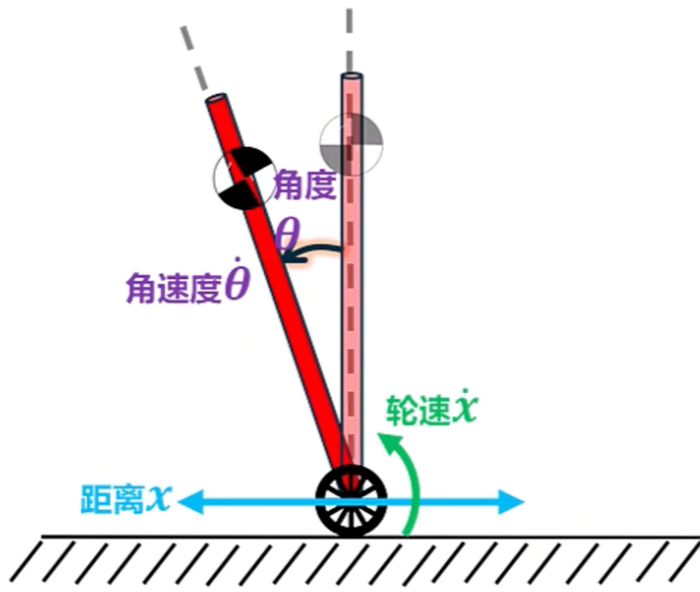
\includegraphics[width=0.5\textwidth]{figures/one_order.png}
  \caption{机器人简化一阶倒立摆示意图}
  \label{fig:one_order}
\end{figure}

\subsection{系统描述与参数定义}
该系统由一个轮子（质量为 $M$）和一个单摆杆（质量为 $m$）组成。我们采用拉格朗日力学法（Lagrange Equation）进行建模。定义系统变量如下：
\begin{table}[H]
  \centering
  \caption{倒立摆参数表}\label{tab:one_order_definition}
  \renewcommand{\arraystretch}{1.3}
  \begin{tabular}{llp{5cm}}
    \toprule
    \textbf{参数} & \textbf{含义}  \\
    \midrule
    $x$ & 轮子中心在水平方向的位移  \\
    $\theta$ & 摆杆相对于垂直向上方向的角度（顺时针为正） \\
    $r$ & 轮子半径 \\
    $h$ & 摆杆质心到旋转轴的距离 \\
    $I$ & 摆杆绕其质心的转动惯量  \\
    $\tau$ & 驱动轮子的电机力矩  \\
    \bottomrule
  \end{tabular}
\end{table}

\subsection{动能与势能分析}
系统的总动能 $T$：
轮子的动能包含平动能与转动能，摆杆的动能由其质心的速度决定。摆杆质心的位置坐标为：
\begin{equation}
  \begin{aligned}
    x_m = x + h\sin\theta \\
    y_m = h\cos\theta
  \end{aligned}
\end{equation}
其速度平方为：
\begin{equation}
v_m^2 = \dot{x}_m^2 + \dot{y}_m^2 = \dot{x}^2 + 2h\dot{x}\dot{\theta}\cos\theta + h^2\dot{\theta}^2
\end{equation}
系统的总动能为：
\begin{equation}
T = \frac{1}{2}(M+m)\dot{x}^2 + \frac{1}{2}(I + mh^2)\dot{\theta}^2 + mh\dot{x}\dot{\theta}\cos\theta
\end{equation}
系统的总势能$V$：
以轮轴为零势能基准面：
\begin{equation}
V = mgh\cos\theta
\end{equation}

\subsection{拉格朗日方程}
定义拉格朗日函数 $L = T - V$。根据拉格朗日方程：
\begin{equation}
\frac{d}{dt}\left(\frac{\partial L}{\partial \dot{q}_i}\right) - \frac{\partial L}{\partial q_i} = Q_i
\end{equation}
其中 $q_i$ 是系统的广义坐标，$Q_i$ 是对应的广义力。对于本系统，选择广义坐标 $q_1 = x$ 和 $q_2 = \theta$，对应的广义力分别为 $Q_1 = \frac{\tau}{r}$（假设轮子与地面之间无滑动）和 $Q_2 = 0$（摆杆不直接受外力矩作用）。通过计算 $\frac{\partial L}{\partial \dot{q}_i}$、$\frac{\partial L}{\partial q_i}$ 和 $\frac{d}{dt}\left(\frac{\partial L}{\partial \dot{q}_i}\right)$，可以得到系统的非线性动力学方程。
其中 $q_1 = x, q_2 = \theta$。对应广义力 $Q_1 = \frac{\tau}{r}$（假设纯滚动），$Q_2 = 0$。
推导得出非线性动力学方程：
\begin{equation}
\begin{cases}
(M + m)\ddot{x} + mh\ddot{\theta}\cos\theta - mh\dot{\theta}^2\sin\theta = \frac{\tau}{r} \\
(I + mh^2)\ddot{\theta} + mh\ddot{x}\cos\theta - mgh\sin\theta = 0
\end{cases}
\end{equation}

\subsection{线性化处理}
在平衡点 $\theta \approx 0$ 附近进行线性化，利用近似条件 $\cos\theta \approx 1, 
\sin\theta \approx \theta, \dot{\theta}^2 \approx 0$：
\begin{equation}
\begin{cases}
(M + m)\ddot{x} + mh\ddot{\theta} = \frac{\tau}{r} \\
mh\ddot{x} + (I + mh^2)\ddot{\theta} - mgh\theta = 0
\end{cases}
\end{equation}

\subsection{状态空间表达式}
令状态向量为 $\mathbf{x} = [\theta, \dot{\theta}, x, \dot{x}]^T$，控制输入 $u = \tau$。联立上述线性方程组，解出 $\ddot{\theta}$ 和 $\ddot{x}$：定义分母行列式：$$D = (M+m)(I+mh^2) - (mh)^2$$整理得到状态空间方程 $\dot{\mathbf{x}} = A\mathbf{x} + Bu$：
\begin{equation}
\begin{bmatrix}
\dot{\theta} \\
\ddot{\theta} \\
\dot{x} \\
\ddot{x}
\end{bmatrix}
=
\begin{bmatrix}
0 & 1 & 0 & 0 \\
\frac{(M+m)mgh}{D} & 0 & 0 & 0 \\
0 & 0 & 0 & 1 \\
-\frac{m^2h^2g}{D} & 0 & 0 & 0
\end{bmatrix}
\begin{bmatrix}
\theta \\
\dot{\theta} \\
x \\
\dot{x}
\end{bmatrix}
+
\begin{bmatrix}
0 \\
-\frac{mh}{Dr} \\
0 \\
\frac{I+mh^2}{Dr}
\end{bmatrix}
\tau
\end{equation}

对于一阶倒立摆（以及更为复杂的轮腿机器人系统），我们通常先证明其开环不稳定但完全可控，进而引入状态反馈（如 LQR 控制器）来实现闭环渐近稳定。以下是为您整理的论文接续内容，您可

\subsection{系统可控性分析}

在设计控制器之前，首先需要判断线性化系统的可控性。对于连续线性时不变系统 $\dot{\mathbf{x}} = A\mathbf{x} + Bu$，其可控性判别矩阵（Controllability Matrix）定义为：
\begin{equation}
Q_c = \begin{bmatrix} B & AB & A^2B & A^3B \end{bmatrix}
\end{equation}

为简化表达，令系统矩阵 $A$ 和输入矩阵 $B$ 中的非零元素分别为：
\begin{equation}
\begin{aligned}
a_{21} &= \frac{(M+m)mgh}{D}, \quad a_{41} = -\frac{m^2h^2g}{D} \\
b_2 &= -\frac{mh}{Dr}, \quad b_4 = \frac{I+mh^2}{Dr}
\end{aligned}
\end{equation}

则矩阵 $A$ 和 $B$ 可简记为：
\begin{equation}
A = \begin{bmatrix} 0 & 1 & 0 & 0 \\ a_{21} & 0 & 0 & 0 \\ 0 & 0 & 0 & 1 \\ a_{41} & 0 & 0 & 0 \end{bmatrix}, \quad B = \begin{bmatrix} 0 \\ b_2 \\ 0 \\ b_4 \end{bmatrix}
\end{equation}

依次计算 $Q_c$ 的各列向量：
\begin{equation}
AB = \begin{bmatrix} b_2 \\ 0 \\ b_4 \\ 0 \end{bmatrix}, \quad A^2B = \begin{bmatrix} 0 \\ a_{21}b_2 \\ 0 \\ a_{41}b_2 \end{bmatrix}, \quad A^3B = \begin{bmatrix} a_{21}b_2 \\ 0 \\ a_{41}b_2 \\ 0 \end{bmatrix}
\end{equation}

由此得到系统的可控性判别矩阵：
\begin{equation}
Q_c = \begin{bmatrix} 0 & b_2 & 0 & a_{21}b_2 \\ b_2 & 0 & a_{21}b_2 & 0 \\ 0 & b_4 & 0 & a_{41}b_2 \\ b_4 & 0 & a_{41}b_2 & 0 \end{bmatrix}
\end{equation}

由于倒立摆系统的物理参数 $M, m, h, I, r$ 均为非零正数，经计算可知该矩阵的行列式 $|Q_c| \neq 0$。因此，可控性矩阵满秩，即 $\text{rank}(Q_c) = 4$。根据卡尔曼秩判据，该一阶倒立摆系统是状态完全可控的，这意味着可以通过设计合适的输入力矩 $\tau$ 来控制系统的所有状态到达期望位置。

\subsection{基于李雅普诺夫理论的稳定性分析}
\subsubsection{开环系统稳定性分析（李雅普诺夫第一方法）}

根据李雅普诺夫间接法（第一方法），线性系统的平衡状态稳定性可由系统矩阵 $A$ 的特征值完全决定。求解矩阵 $A$ 的特征方程：
\begin{equation}
|\lambda I - A| = \begin{vmatrix} \lambda & -1 & 0 & 0 \\ -a_{21} & \lambda & 0 & 0 \\ 0 & 0 & \lambda & -1 \\ -a_{41} & 0 & 0 & \lambda \end{vmatrix} = \lambda^2 (\lambda^2 - a_{21}) = 0
\end{equation}

解得系统的四个开环特征值（极点）为：
\begin{equation}
\lambda_1 = 0, \quad \lambda_2 = 0, \quad \lambda_3 = \sqrt{a_{21}}, \quad \lambda_4 = -\sqrt{a_{21}}
\end{equation}

由于物理参数决定的 $a_{21} = \frac{(M+m)mgh}{D} > 0$，因此 $\lambda_3$ 为正实数。根据李雅普诺夫第一方法，若系统矩阵存在实部大于零的特征值，则该系统在平衡点处是李雅普诺夫不稳定的。这与倒立摆在无控制作用下会自然倾倒的物理直觉相符。

\subsubsection{闭环系统渐近稳定与状态反馈设计（李雅普诺夫第二方法）}
为了使系统稳定在倒立平衡点，需引入状态反馈控制。考虑采用线性二次型调节器（LQR）设计最优控制律：
\begin{equation}
u = -K\mathbf{x}
\end{equation}

其中，$K$ 为状态反馈增益矩阵。此时闭环系统状态方程变为：
\begin{equation}
\dot{\mathbf{x}} = (A - BK)\mathbf{x} = A_{cl}\mathbf{x}
\end{equation}

根据李雅普诺夫直接法（第二方法），构造正定二次型李雅普诺夫函数：
\begin{equation}
V(\mathbf{x}) = \mathbf{x}^T P \mathbf{x}
\end{equation}

其中 $P$ 为对称正定矩阵。对其求时间导数：
\begin{equation}
\dot{V}(\mathbf{x}) = \dot{\mathbf{x}}^T P \mathbf{x} + \mathbf{x}^T P \dot{\mathbf{x}} = \mathbf{x}^T (A_{cl}^T P + P A_{cl}) \mathbf{x}
\end{equation}

为保证系统在平衡点处大范围渐近稳定，要求 $\dot{V}(\mathbf{x})$ 为负定，即存在对称正定矩阵 $Q$，满足连续代数黎卡提方程：
\begin{equation}
A_{cl}^T P + P A_{cl} = -Q
\end{equation}

由于系统已证明为完全可控，对于任意给定的半正定状态权重矩阵 $Q$ 和正定控制权重矩阵 $R$，必然存在唯一正定解 $P$，使得通过 $K = R^{-1}B^T P$ 得到的闭环矩阵 $A_{cl}$ 的所有特征值均位于左半复平面。由此，通过 LQR 等状态反馈控制，开环不稳定的倒立摆系统能够被镇定，实现闭环渐近稳定。

\section{电缆通道检测机器人的控制方案设计}
基于上述对一阶倒立摆模型的分析，我们设计了一个基于状态反馈的控制方案。具体是基于LQR控制算法实现对机器人状态的反馈控制，LQR输出为轮电机扭矩以及腿对底盘的等效力矩。

然后通过VMC方法将腿对底盘的等效力和等效力矩转化为两个关节电机的控制输入。

具体步骤如下：

1. 选择合适的状态权重矩阵 $Q$ 和控制权重矩阵 $R$，以平衡系统状态误差和控制输入的大小。

2. 通过求解连续代数黎卡提方程得到最优状态反馈增益矩阵 $K$。

3. 实现控制律 $u = -K\mathbf{x}$，将系统状态反馈到控制输入中，以实现对系统的稳定控制。

\section{控制器设计}
机器人控制解耦为运动控制（Locomotion Controller）和腿部控制（Leg Controller）两部分。运动控制器通过调节驱动轮转矩和腿部关节转矩使机器人保持平衡和控制机器人移动、旋转；腿部控制器通过调节腿部支持力控制腿长，使机器人保持滚转（roll）方向稳定，并起到主动悬挂的作用。

\subsection{运动控制器 (Locomotion Controller)}
根据状态空间模型设计状态反馈控制器

状态反馈控制器
\begin{equation}
u = K_{4 \times 10}(x_d - x) 
\end{equation}

状态反馈矩阵 $K$ 通过 Linear Quadratic Regulator (LQR) 计算得到，代价函数
\begin{equation}
J = \int_{0}^{\infty} (x^T Q x + u^T R u) dt 
\end{equation}

根据 LQR 可以得到状态反馈矩阵 $K$
\begin{equation}
K = R^{-1} B^T P 
\end{equation}

其中 $P$ 满足 Riccati 方程
\begin{equation}
A^T P + P A - P B R^{-1} B^T P + Q = 0 
\end{equation}

式 (3.4) 中，$A, B$ 是关于腿长 $l$ 的函数，为了降低运算量，在工作空间内采用多项式拟合的方式得到状态反馈矩阵 $K$
\begin{equation}
K(l_l, l_r) = K_{K,1} + K_{K,2} l_l + K_{K,3} l_l^2 + K_{K,4} l_r + K_{K,5} l_r^2 + K_{K,6} l_l l_r 
\end{equation}

\subsection{腿部控制器 (Leg Controller)}
控制目标：调节腿部支持力控制左右腿长度，使机体保持特定高度 \& 滚转角，并起到悬挂减震的作用

输入：机体目标滚转角(roll) \& 目标腿长(平均值) $(\psi_d, l_d)$

输出：左右腿支持力 $(F_{bl,l}, F_{bl,r})$

反馈：机体滚转角 \& 左右腿长度 $(\psi, l_l, l_r)$

控制器：单环PID控制（PD模拟弹簧阻尼系统，消除前馈误差）+ 前馈（重力+侧向惯性力矩补偿）

重力补偿前馈
\begin{equation}
F_{ff,gravity} = \left(\frac{1}{2}m_b + \eta m_l\right)g 
\end{equation}

侧向惯性力矩补偿前馈
\begin{equation}
F_{ff,inertial} = \left(\frac{1}{2}m_b + \eta m_l\right) \frac{l}{2} \ddot{\psi} 
\end{equation}

最终左右腿支持力
\begin{equation}
\begin{bmatrix}
F_{bl,l} \\
F_{bl,r}
\end{bmatrix} = 
\begin{bmatrix}
1 & 1 & 1 & -1 \\
-1 & 1 & 1 & 1
\end{bmatrix}
\begin{bmatrix}
F_\psi \\
F_l \\
F_{ff,gravity} \\
F_{ff,inertial}
\end{bmatrix}
\end{equation}
% <<< END INPUT chapters/09_control.tex
% >>> BEGIN INPUT chapters/10_control_simulation.tex
\chapter{运动控制仿真}\label{chap:control_simulation}
\section{仿真环境与工具选择}
为了验证前一章设计的控制方案的有效性，我们选择了MATLAB/Simulink作为仿真平台。MATLAB提供了强大的数值计算能力和丰富的工具箱，Simulink则支持基于模型的设计和仿真，能够直观地构建系统模型并进行动态仿真。此外，我们还利用了Simscape Multibody模块来建立机器人动力学模型。
\section{控制方案仿真设计}
仿真设计分为以下几个步骤：

1）建立机器人动力学模型：基于前一章的建模结果，我们在Simscape Multibody中构建了轮腿式机器人的动力学模型，包含底盘、腿部结构以及轮子等关键组件。

2）实现控制算法：根据前一章设计的控制方案，我们在Simulink中实现了相应的控制算法，从LQR输出腿部等效力和力矩，再通过VMC转化到轮电机和关节电机的控制输入。

3）设置仿真场景：为了测试控制方案的性能，本毕业设计设计了多个仿真场景，包括平坦地面、带有障碍物的环境，以评估机器人在不同环境下的运动控制能力。

4）运行仿真并收集数据：通过运行仿真，我们收集了机器人在不同场景下的电机控制输入和状态量的输出数据。

\section{控制框架设计}
\begin{figure}[H]
  \centering
  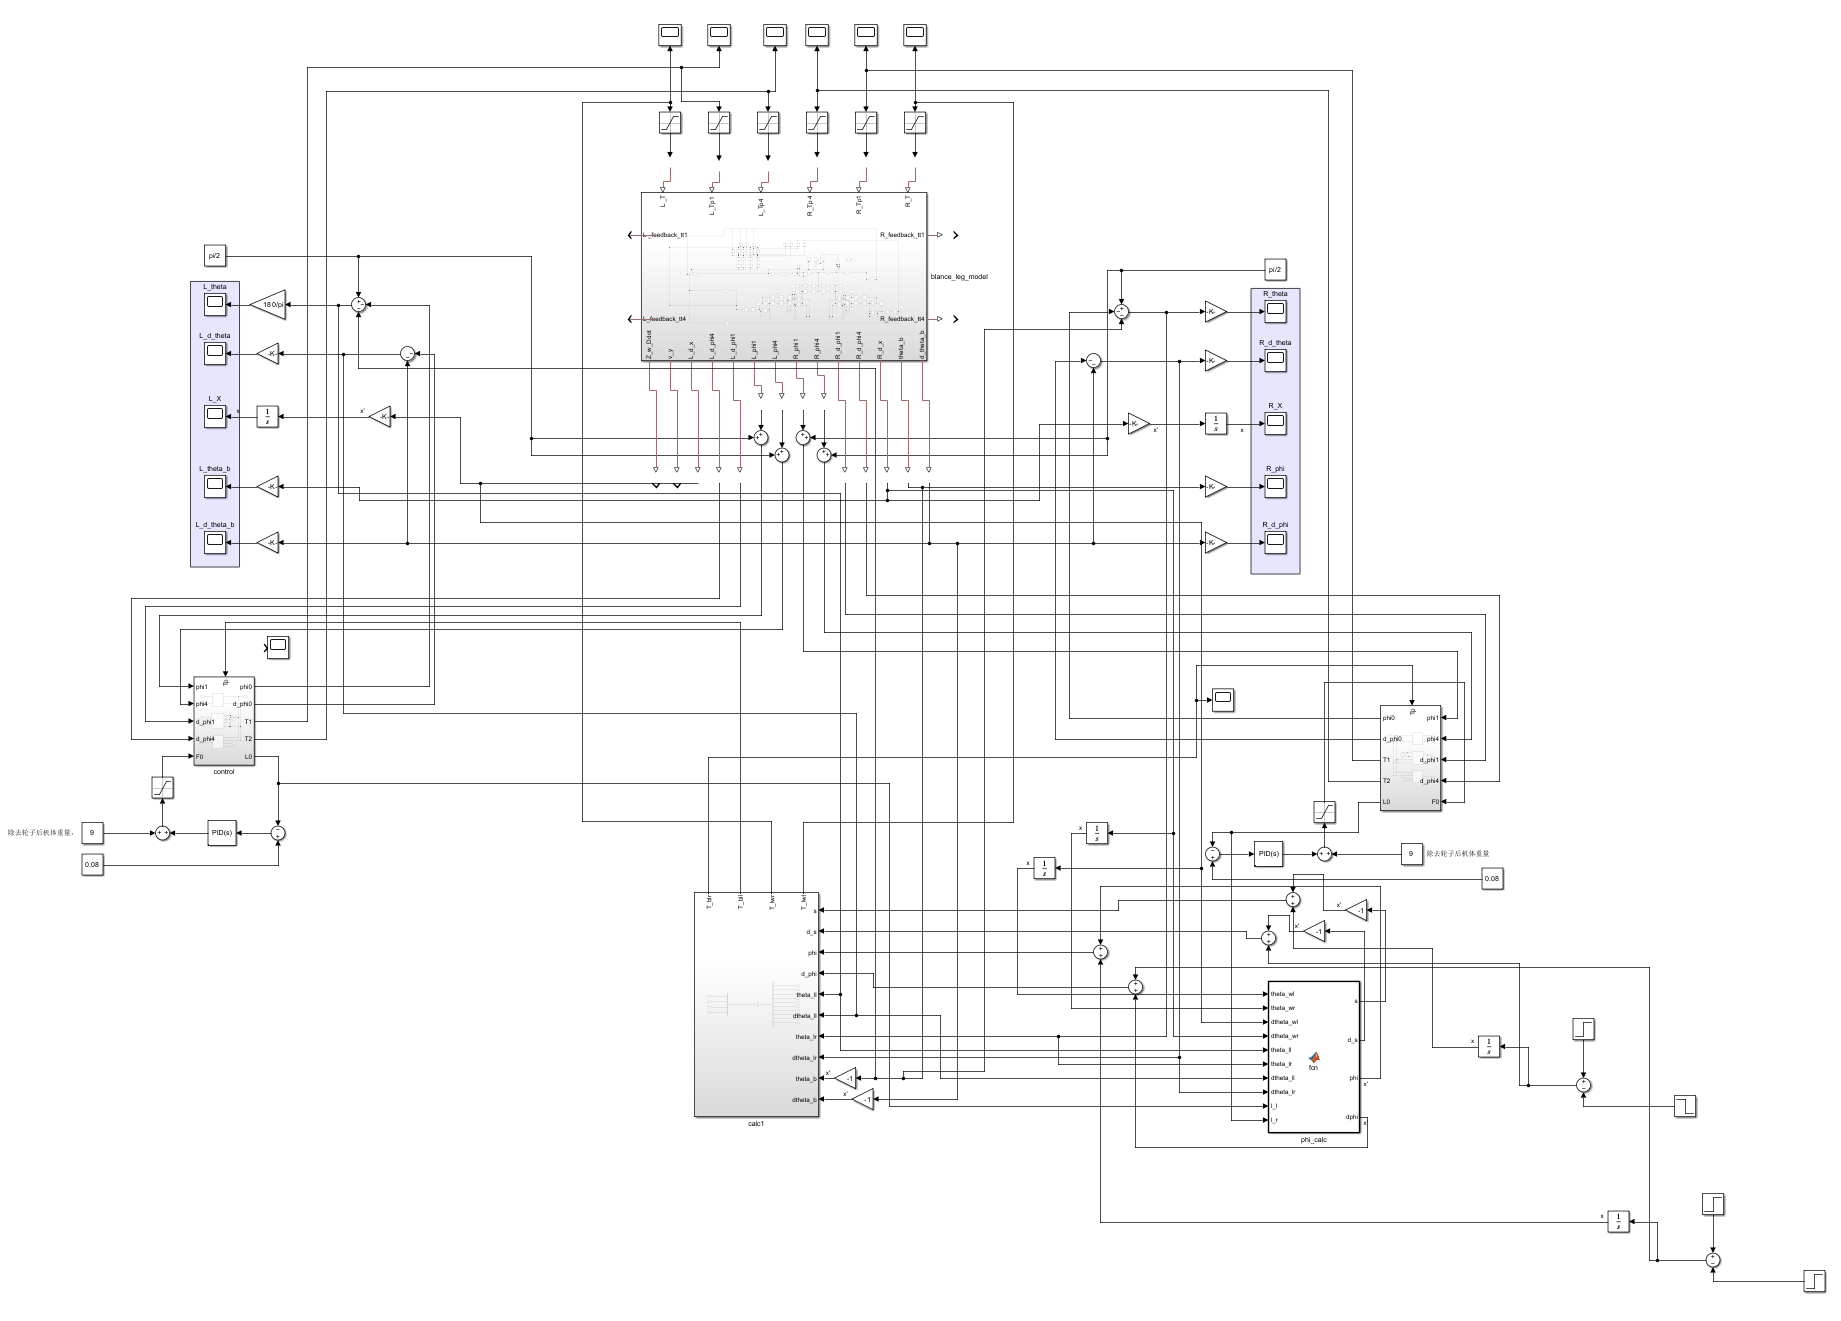
\includegraphics[width=0.9\textwidth]{figures/control_framework.png}
  \caption{控制框架设计}
  \label{fig:control-framework}
\end{figure}
在simulink中搭建了一个控制框架，如图\ref{fig:control-framework}所示。该框架包括以下几个模块：
\subsection{仿真环境搭建}
\begin{figure}[H]
  \centering
  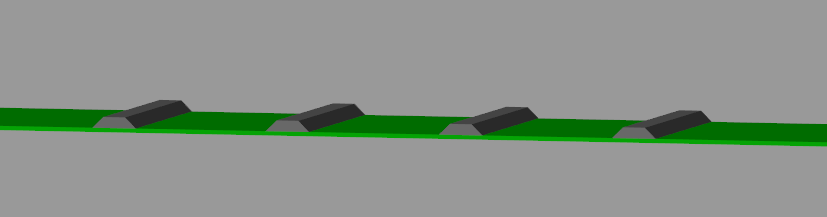
\includegraphics[width=0.9\textwidth]{figures/simulink_env.png}
  \caption{仿真环境搭建}
  \label{fig:simulation-environment}
\end{figure}

\begin{figure}[H]
  \centering
  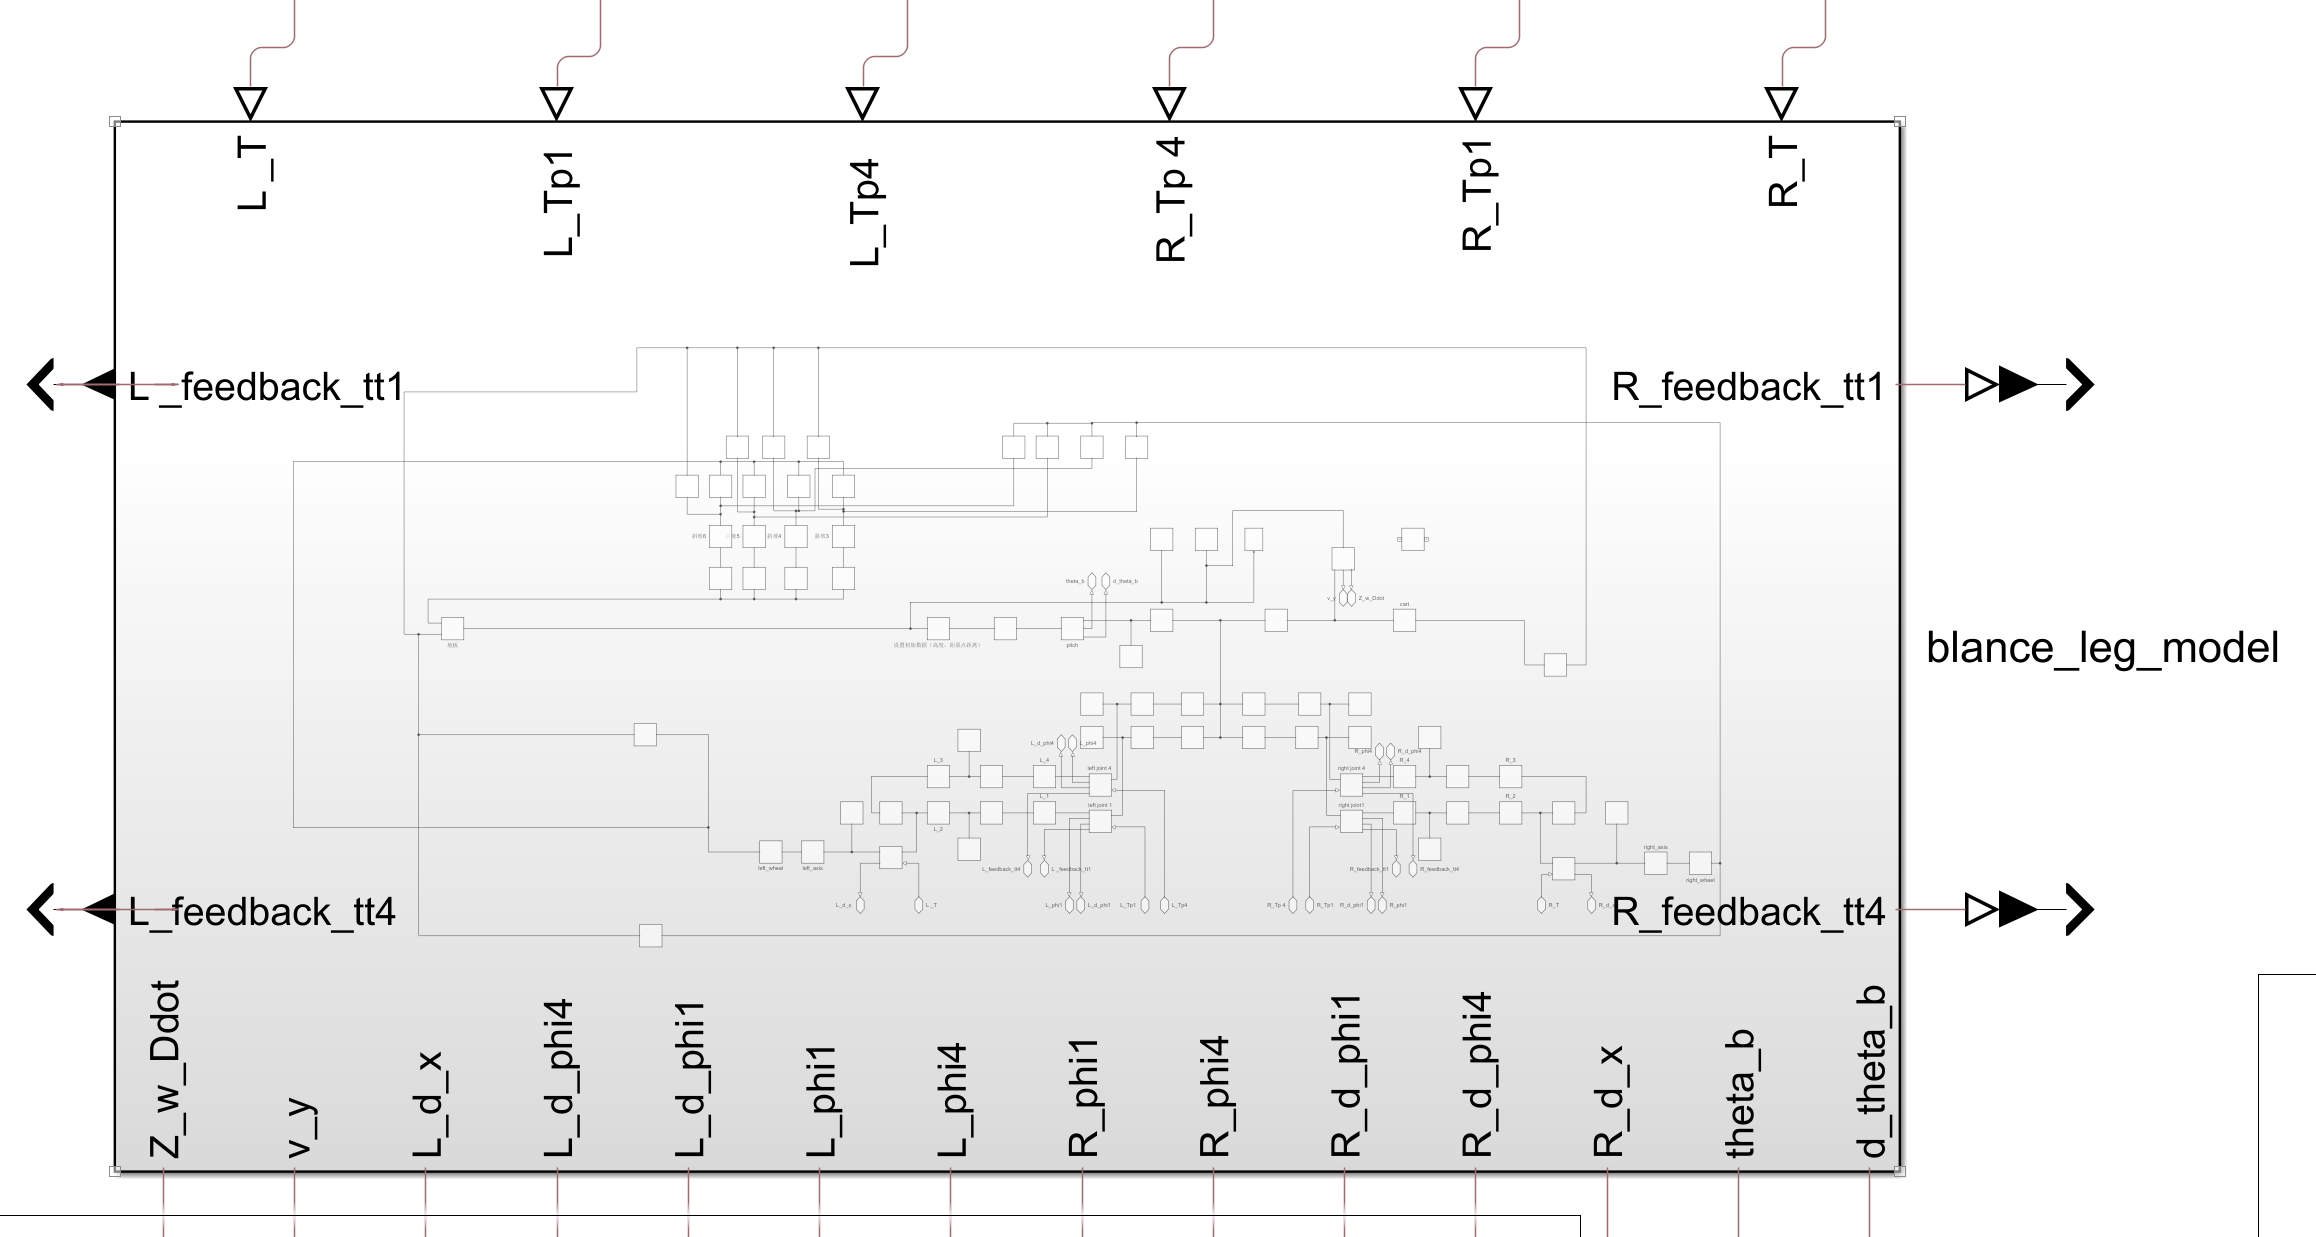
\includegraphics[width=0.7\textwidth]{figures/model_simulink_outside.png}
  \caption{轮腿机器人建模外部接口}
  \label{fig:model-simulink-outside}
\end{figure}

\begin{figure}[H]
  \centering
  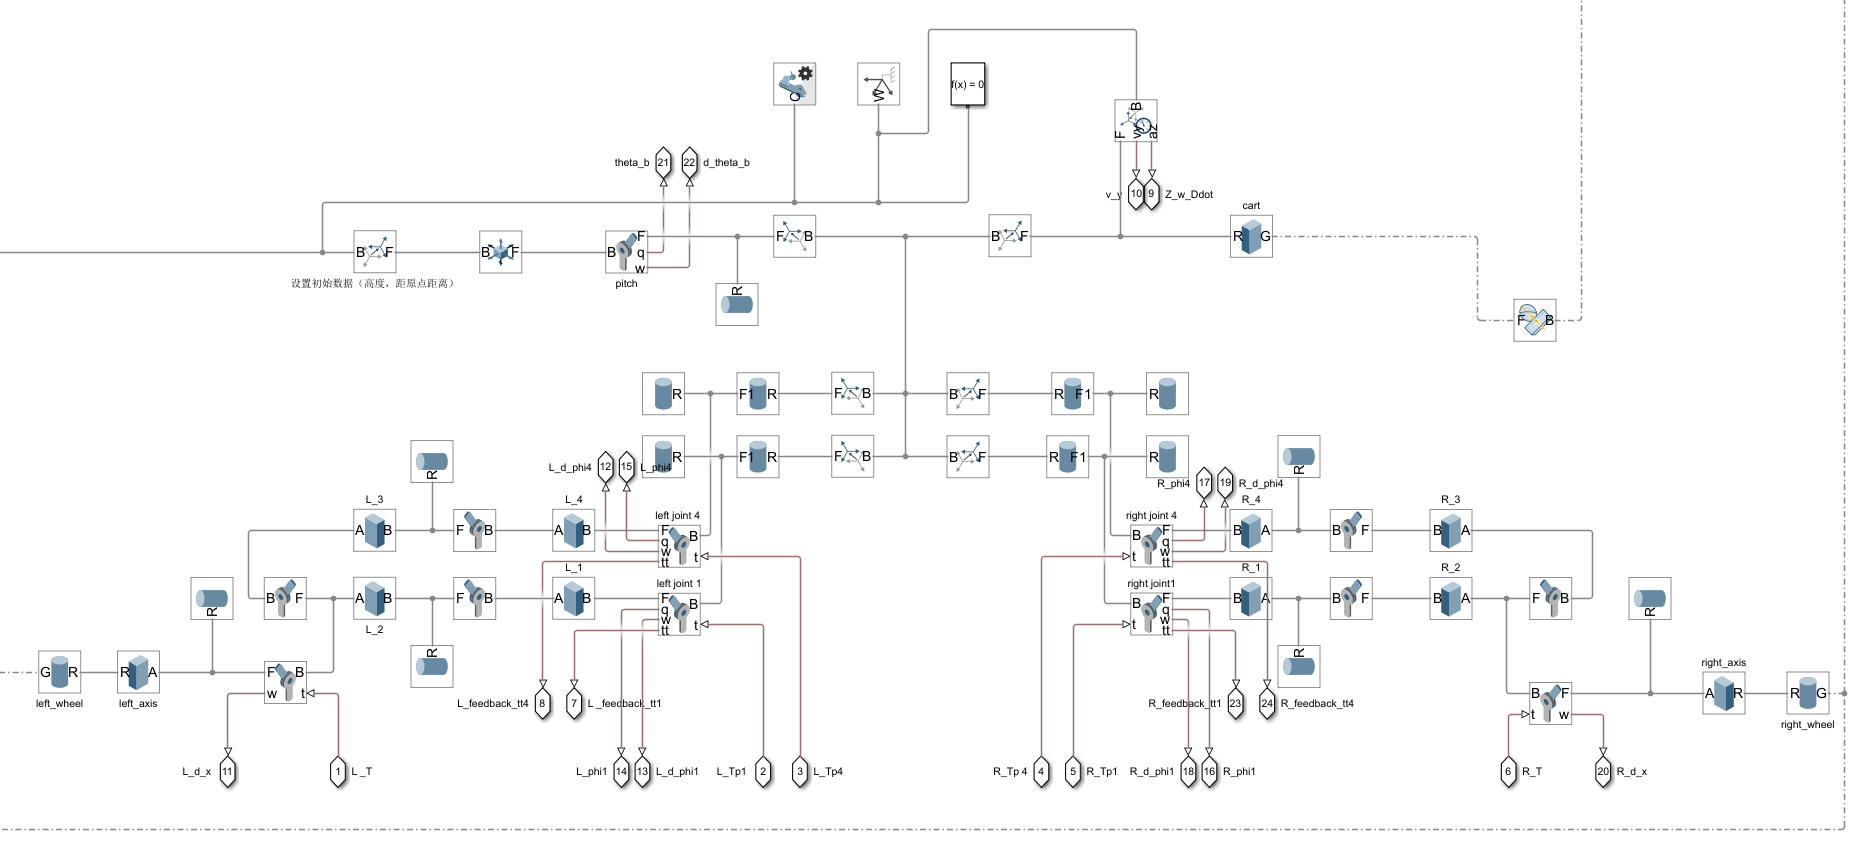
\includegraphics[width=0.7\textwidth]{figures/model_simulink_inside.png}
  \caption{轮腿机器人建模内部实现}
  \label{fig:model-simulink-inside}
\end{figure}

\begin{figure}[H]
  \centering
  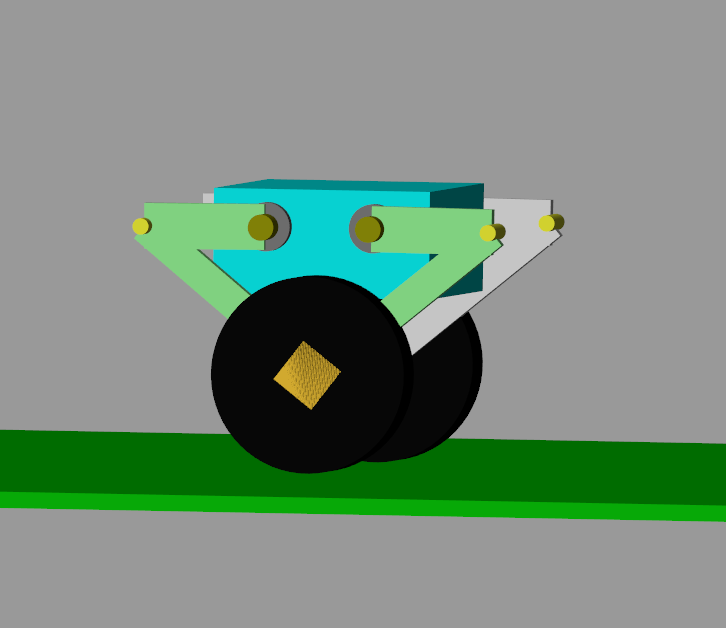
\includegraphics[width=0.5\textwidth]{figures/simulink_model.png}
  \caption{机器人建模}
  \label{fig:robot-model}
\end{figure}

\subsection{lqr控制模块}
\begin{figure}[H]
  \centering
  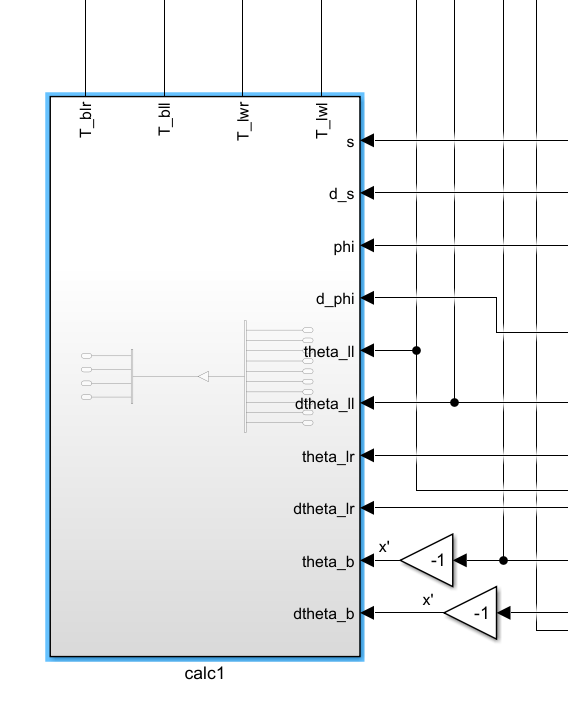
\includegraphics[width=0.3\textwidth]{figures/lqr_outside.png}
  \caption{lqr控制器外部接口}
  \label{fig:lqr-outside}
\end{figure}

\begin{figure}[H]
  \centering
  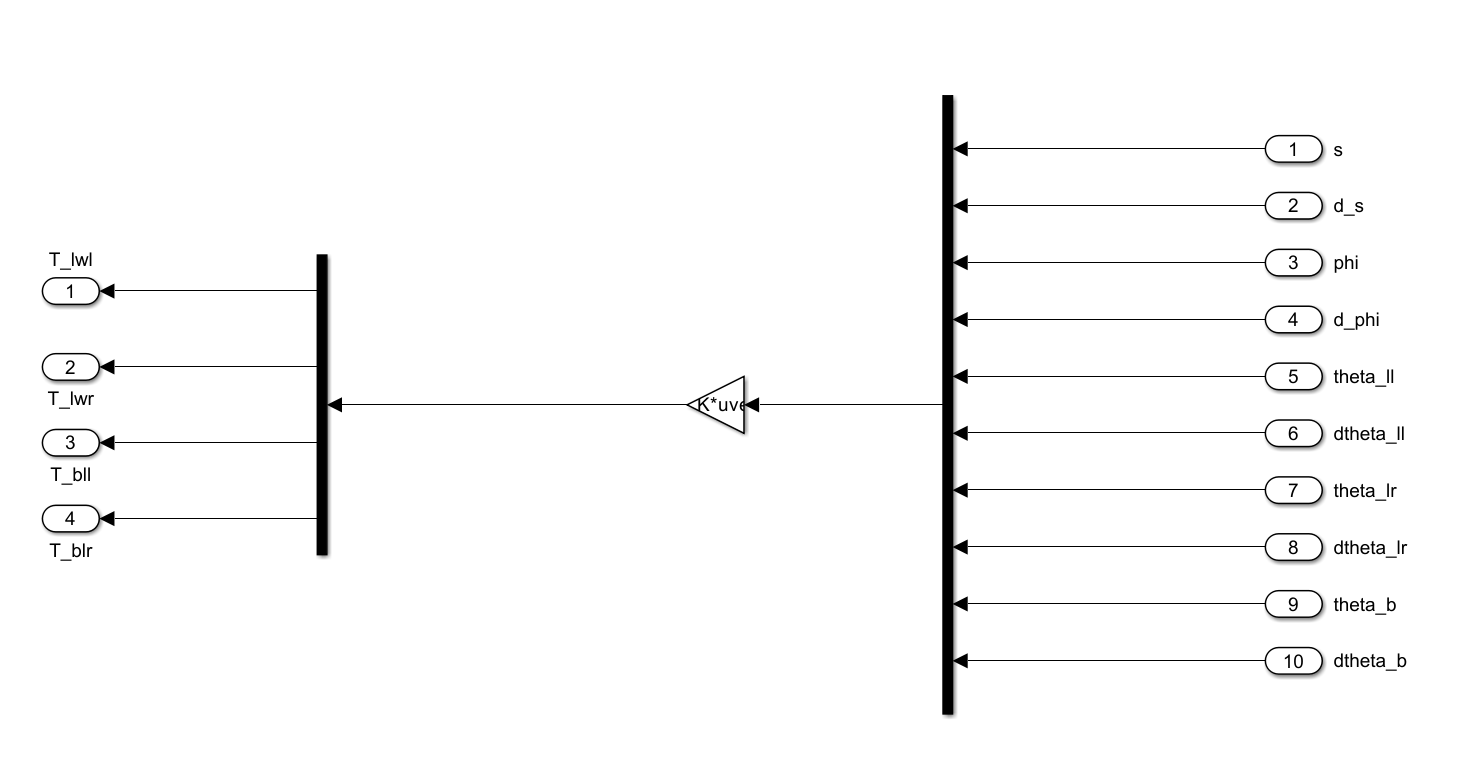
\includegraphics[width=0.9\textwidth]{figures/lqr_inside.png}
  \caption{lqr控制器内部实现}
  \label{fig:lqr-inside}
\end{figure}

LQR控制模块通过系统状态量的输入乘已经计算好的K矩阵该模块的输入包括机器人水平位移、水平位移速度、机器人yaw转角、yaw转角速度、腿部摆杆角度、腿部摆杆角速度、机体倾角、机体倾角速度状态量，输出腿部等效力矩和轮电机力矩。

\subsection{状态量求解与VMC}
\begin{figure}[H]
  \centering
  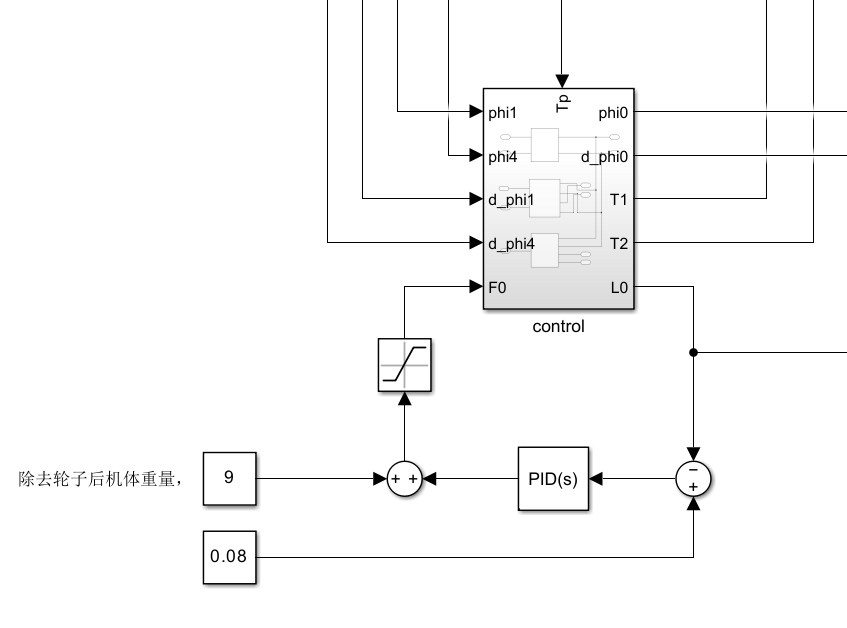
\includegraphics[width=0.5\textwidth]{figures/control_state_vmc_outside.png}
  \caption{状态量求解与VMC转化外部接口}
  \label{fig:state-and-vmc-outside}
\end{figure}

\begin{figure}[H]
  \centering
  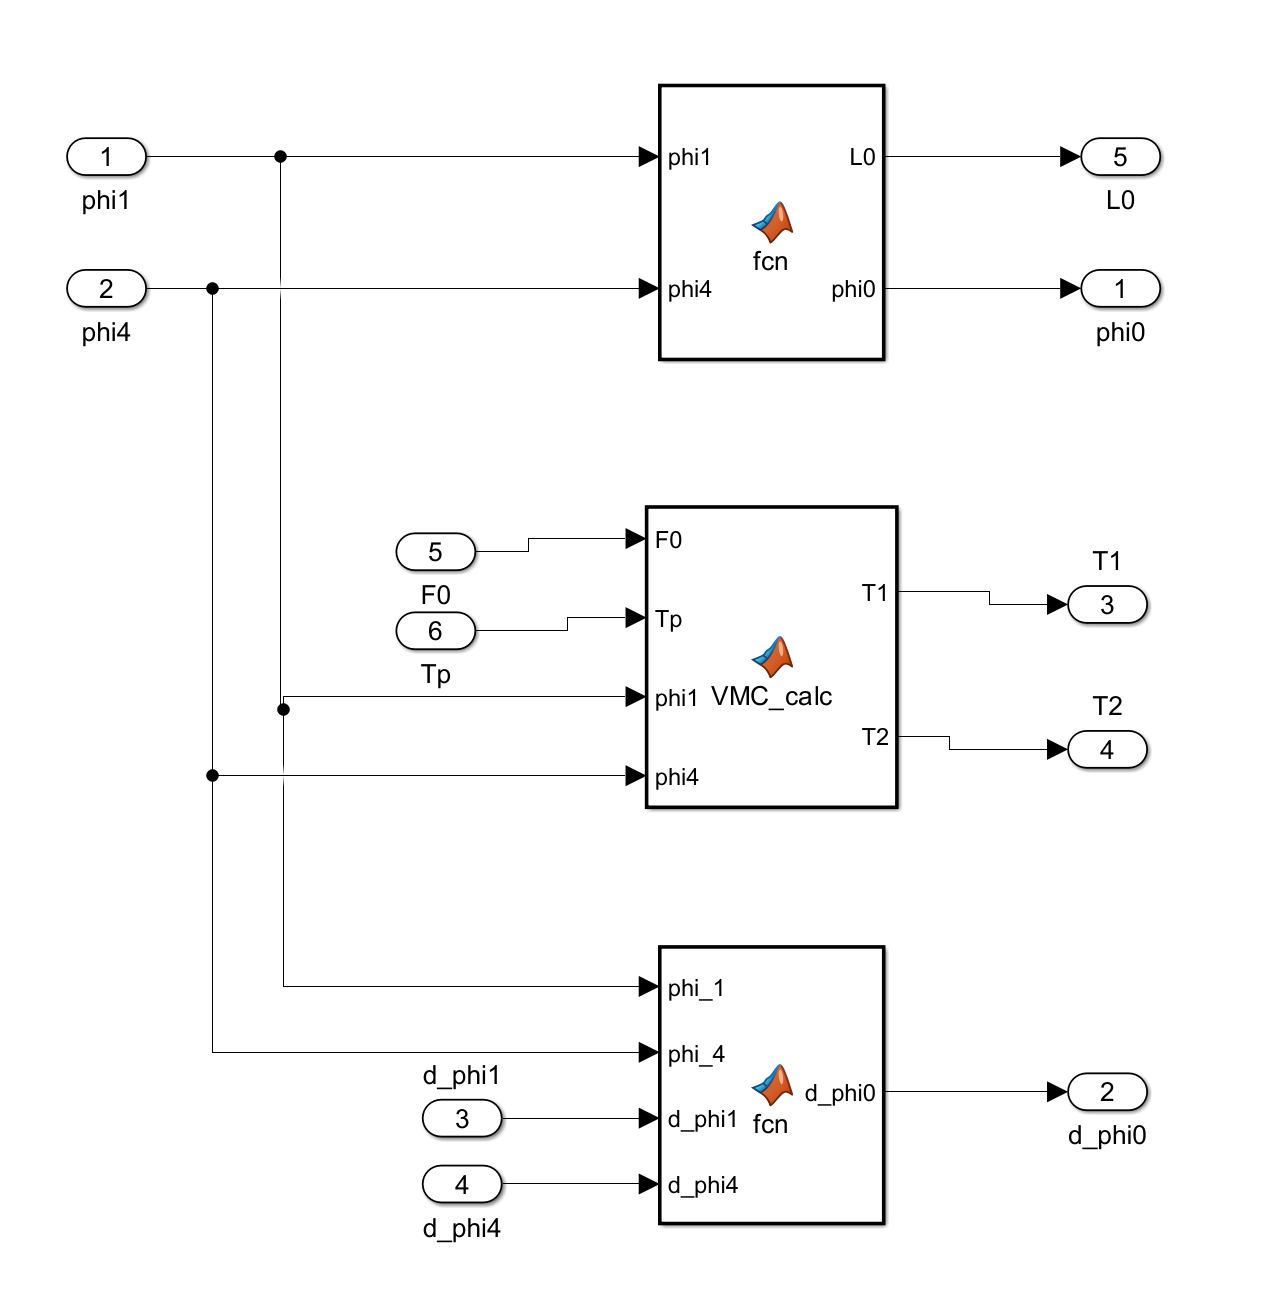
\includegraphics[width=0.5\textwidth]{figures/control_state_vmc_inside.png}
  \caption{状态量求解与VMC转化内部实现}
  \label{fig:state-and-vmc-inside}
\end{figure}

该模块的作用为通过 $\phi_1$、$\phi_4$，经过几何解算求得 $L_0$ 和 $\phi_0$，同时可再结合 $F_0$ 和 $T_p$ 通过 VMC 转化求得两个关节电机的控制输入。同时还通过雅各比矩阵求得 $\dot{\phi}_0$，便于后续继续求解腿角速度等。

\subsubsection{五连杆运动学解算}

\begin{minted}[breaklines,linenos,fontsize=\small]{matlab}
function [L0,phi0] = fcn(phi1,phi4)
   
    l5=0.08;%AE长度
    l1=0.075;
    l2=0.14;
    l3=0.14;
    l4=0.075;
    
    YD = l4*sin(phi4);
    YB = l1*sin(phi1);
    XD = l5 + l4*cos(phi4);
    XB = l1*cos(phi1); 
    lBD = sqrt((XD - XB)*(XD - XB) + (YD - YB)*(YD - YB));
    A0 = 2*l2*(XD - XB);
    B0 = 2*l2*(YD - YB);
    C0 = l2*l2 + lBD*lBD - l3*l3;
    phi2 = 2*atan2((B0 + sqrt(A0*A0 + B0*B0 - C0*C0)),(A0 + C0));
    XC = l1*cos(phi1) + l2*cos(phi2);
    YC = l1*sin(phi1) + l2*sin(phi2);
    L0 = sqrt((XC - l5/2)*(XC - l5/2) + YC*YC);
    phi0=atan2(YC,(XC-l5/2));
    
end
\end{minted}

\subsubsection{VMC解算}

\begin{minted}[breaklines,linenos,fontsize=\small]{matlab}
function [T1,T2] = VMC_calc(F0,Tp,phi1,phi4)

    l5=0.08;%AE长度
    l1=0.075;
    l2=0.14;
    l3=0.14;
    l4=0.075;

YD = l4*sin(phi4);
YB = l1*sin(phi1);
XD = l5 + l4*cos(phi4);
XB = l1*cos(phi1); 
lBD = sqrt((XD - XB)*(XD - XB) + (YD - YB)*(YD - YB));
A0 = 2*l2*(XD - XB);
B0 = 2*l2*(YD - YB);
C0 = l2*l2 + lBD*lBD - l3*l3;
phi2 = 2*atan2((B0 + sqrt(A0*A0 + B0*B0 - C0*C0)),A0 + C0);
phi3 = atan2(YB-YD+l2*sin(phi2),XB-XD+l2*cos(phi2));
XC = l1*cos(phi1) + l2*cos(phi2);
YC = l1*sin(phi1) + l2*sin(phi2);
L0 = sqrt((XC - l5/2)*(XC - l5/2) + YC*YC);
phi0 = atan2(YC,XC - l5/2);
j11 = (l1*sin(phi0-phi3)*sin(phi1-phi2))/sin(phi3-phi2);
j12 = (l1*cos(phi0-phi3)*sin(phi1-phi2))/(L0*sin(phi3-phi2));
j21 = (l4*sin(phi0-phi2)*sin(phi3-phi4))/sin(phi3-phi2);
j22 = (l4*cos(phi0-phi2)*sin(phi3-phi4))/(L0*sin(phi3-phi2));
J = [j11 j12; j21 j22];
F = [F0;Tp];
T = J * F;
T1 = T(1,1);
T2 = T(2,1);
end
\end{minted}

\subsubsection{不含机体倾角速度的腿角速度求解}

\begin{minted}[breaklines,linenos,fontsize=\small]{matlab}
function d_phi0 = fcn(phi_1, phi_4, d_phi1, d_phi4)
    % --- 几何参数 ---
    l5 = 0.08;  % 机身基座宽度 (AE)
    l1 = 0.075; % 主动臂1
    l2 = 0.14;  % 连杆2
    l3 = 0.14;  % 连杆3
    l4 = 0.075; % 主动臂4

    % --- 1. 正运动学求解 ---
    % A点在 (0,0), E点在 (l5, 0)
    % B点坐标 (主动臂1末端)
    xB = l1 * cos(phi_1);
    yB = l1 * sin(phi_1);
    
    % D点坐标 (主动臂4末端)
    xD = l5 + l4 * cos(phi_4);
    yD = l4 * sin(phi_4);

    % 求解 B, D 两圆交点 C (足端)
    distBD = sqrt((xD - xB)^2 + (yD - yB)^2);
    a = (l2^2 - l3^2 + distBD^2) / (2 * distBD);
    h = sqrt(max(0, l2^2 - a^2));
    
    x2 = xB + a * (xD - xB) / distBD;
    y2 = yB + a * (yD - yB) / distBD;
    
    % 足端 C 的坐标 
    xc = x2 + h * (yD - yB) / distBD;
    yc = y2 - h * (xD - xB) / distBD;

    % 计算被动段角度 phi2, phi3
    phi_2 = atan2(yc - yB, xc - xB);
    phi_3 = atan2(yc - yD, xc - xD);

    % --- 2. 雅可比矩阵求解 ---
    sin_diff = sin(phi_2 - phi_3);
    J11 = l1 * sin(phi_1 - phi_3) * cos(phi_2) / sin_diff; 
    J12 = l4 * sin(phi_4 - phi_2) * cos(phi_3) / sin_diff;
    J21 = l1 * sin(phi_1 - phi_3) * sin(phi_2) / sin_diff;
    J22 = l4 * sin(phi_4 - phi_2) * sin(phi_3) / sin_diff;
    
    dxc = J11 * d_phi1 + J12 * d_phi4;
    dyc = J21 * d_phi1 + J22 * d_phi4;

    % --- 3. 计算腿部摆动角速度 ---
    l02 = xc^2 + yc^2;    
    d_phi0 = (xc * dyc - yc * dxc) / l02;
end
\end{minted}

\section{仿真参数配置}

本仿真在MATLAB R2024a环境下进行，使用Simulink 10.0版本。仿真时间设置为10秒，求解器为ode45变步长。机器人初始状态设定为距离地面高度30cm处落下，随后在1s和5s时间点处给定速度激励1m/s和-1m/s。仿真场景包括前半段的平坦地面和连续四个高度为0.25米的障碍物，机器人需要从初始状态落下到起点并越过障碍物，期间保持机体稳定不发散。

控制器参数设置如下：LQR权重矩阵$Q$设定为对状态量的单位矩阵，控制输入权重矩阵$R$设定为对控制输入的单位矩阵。仿真过程中，机器人需要根据控制器输出的力矩调整轮电机和关节电机的输入，以实现稳定的运动控制。
\begin{minted}[breaklines,linenos,fontsize=\small]{matlab}
%        s     ds     phi     dphi     theta_ll dtheta_ll theta_lr dtheta_lr theta_b dtheta_b
lqr_Q = [10,    0,     0,      0,       0,       0,       0,      0,       0,       0;
         0,    5,     0,      0,       0,       0,        0,       0,        0,       0;
         0,    0,     10,      0,       0,       0,       0,      0,       0,       0;
         0,    0,     0,      5,       0,       0,        0,       0,        0,       0;
         0,    0,     0,      0,       1,       0,        0,       0,        0,       0;
         0,    0,     0,      0,       0,       0.07,     0,       0,        0,       0;
         0,    0,     0,      0,       0,       0,        1,       0,        0,       0;
         0,    0,     0,      0,       0,       0,        0,       0.07,     0,       0;
         0,    0,     0,      0,       0,       0,        0,       0,        10,       0;
         0,    0,     0,      0,       0,       0,        0,       0,        0,      0.6];
% 其中：
% s       : 自然坐标系下机器人水平方向移动距离，单位：m，ds为其导数
% phi     ：机器人水平方向移动时yaw偏航角度，dphi为其导数
% theta_ll：左腿摆杆与竖直方向（自然坐标系z轴）夹角，dtheta_ll为其导数
% theta_lr：右腿摆杆与竖直方向（自然坐标系z轴）夹角，dtheta_lr为其导数
% theta_b ：机体与自然坐标系水平夹角，dtheta_b为其导数

% 矩阵中，以下列分别对应：
%        T_wl    T_wr     T_bl     T_br
lqr_R = [20,      0,       0,       0;
         0,      20,       0,       0;
         0,      0,       10,       0;
         0,      0,       0,       10];
\end{minted}

\section{仿真结果分析}
\begin{figure}[H]
  \centering
  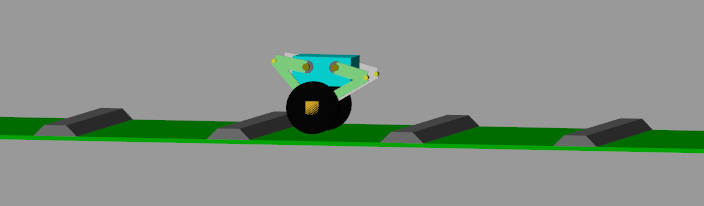
\includegraphics[width=0.5\textwidth]{figures/obstacle_1.png}
  \caption{越障前的机器人状态}
  \label{fig:obstacle-1}
\end{figure}
\begin{figure}[H]
  \centering
  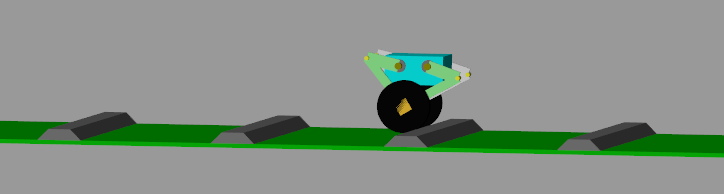
\includegraphics[width=0.5\textwidth]{figures/obstacle_2.png}
  \caption{越障中的机器人状态1}
  \label{fig:obstacle-2}
\end{figure}
\begin{figure}[H]
  \centering
  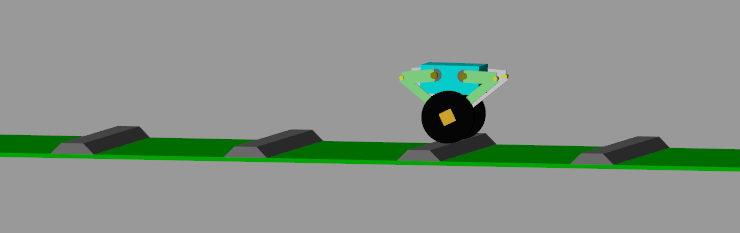
\includegraphics[width=0.5\textwidth]{figures/obstacle_3.png}
  \caption{越障中的机器人状态2}
  \label{fig:obstacle-3}
\end{figure}
\begin{figure}[H]
  \centering
  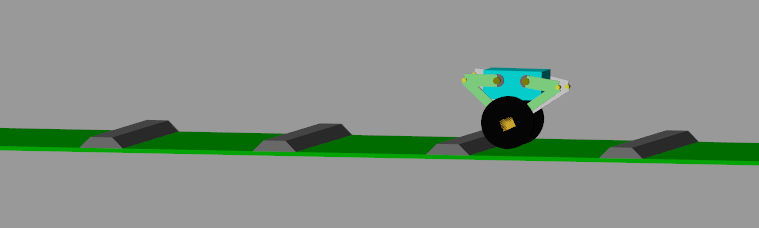
\includegraphics[width=0.5\textwidth]{figures/obstacle_4.png}
  \caption{越障后的机器人状态}
  \label{fig:obstacle-4}
\end{figure}
\begin{figure}[H]
  \centering
  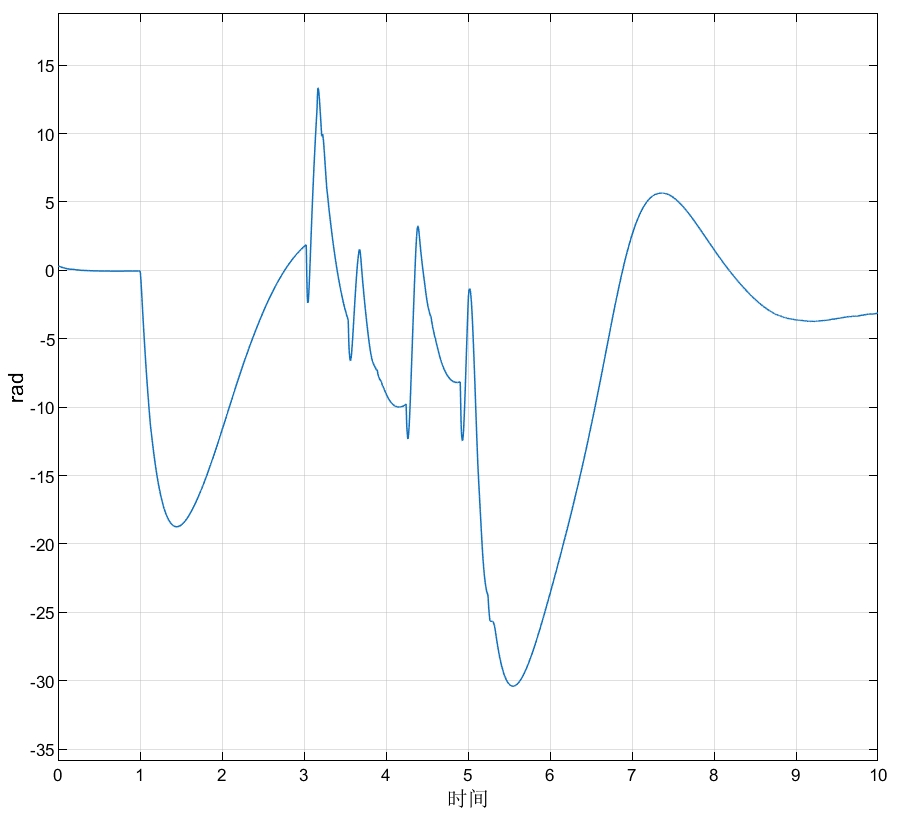
\includegraphics[width=0.5\textwidth]{figures/simulink_theta.png}
  \caption{状态量腿角度变化曲线}
  \label{fig:theta}
\end{figure}
\begin{figure}[H]
  \centering
  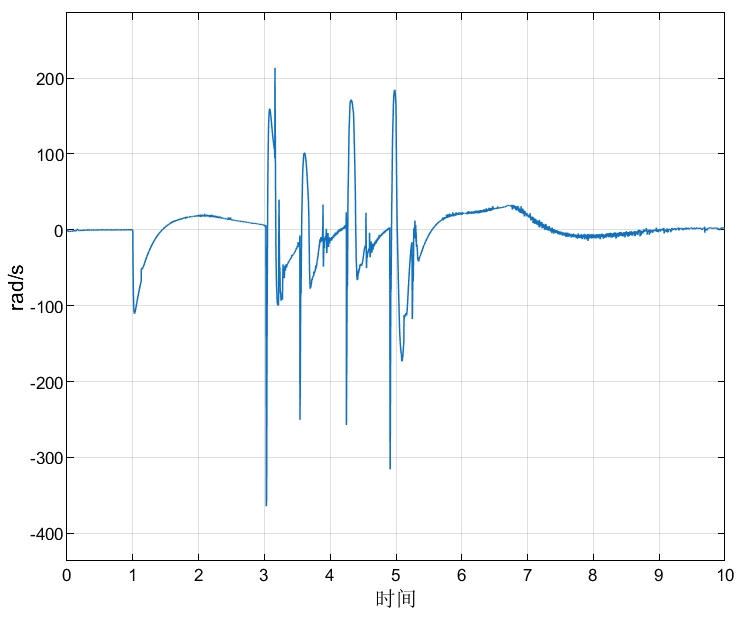
\includegraphics[width=0.5\textwidth]{figures/simulink_dtheta.png}
  \caption{状态量腿角速度变化曲线}
  \label{fig:dtheta}
\end{figure}
\begin{figure}[H]
  \centering
  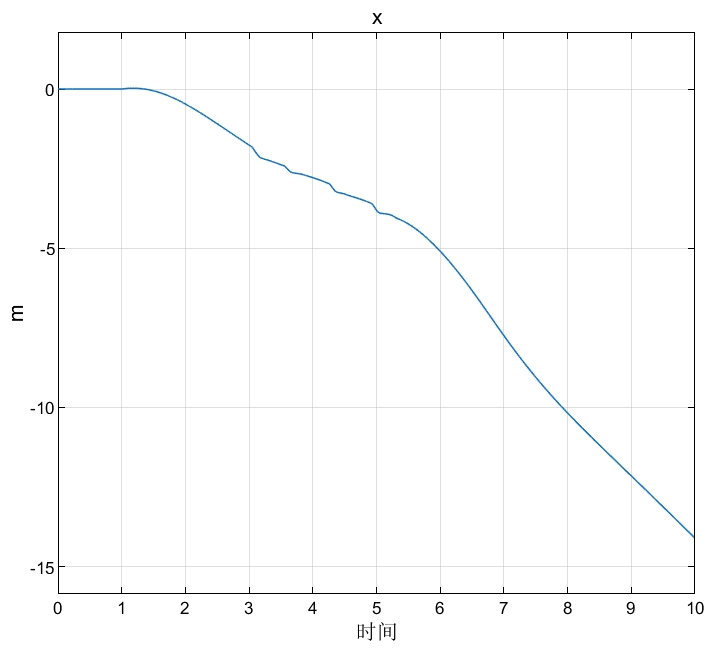
\includegraphics[width=0.5\textwidth]{figures/simulink_x.png}
  \caption{状态量机器人水平位移变化曲线}
  \label{fig:x}
\end{figure}
\begin{figure}[H]
  \centering
  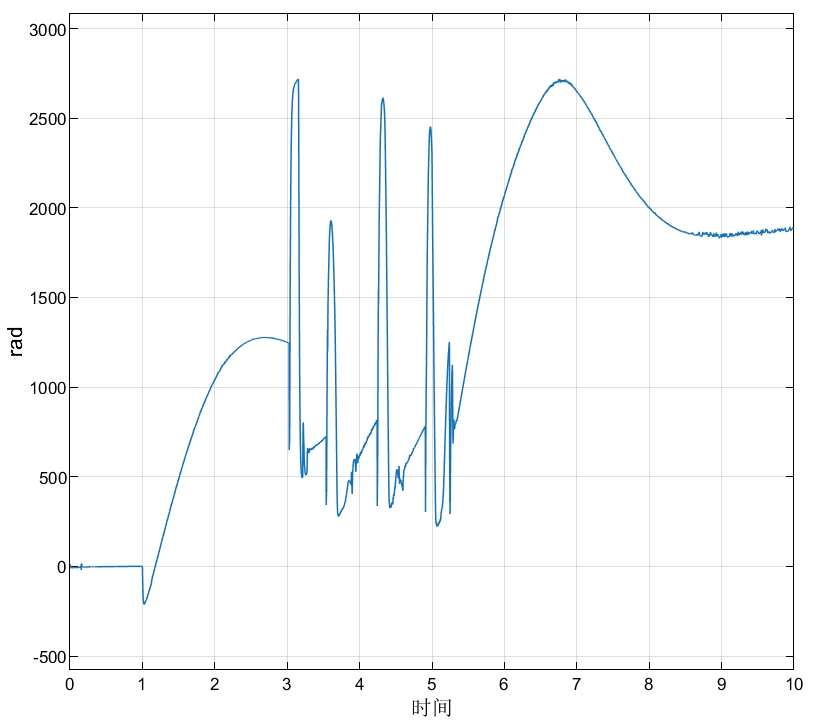
\includegraphics[width=0.5\textwidth]{figures/simulink_theta_b.png}
  \caption{状态量机体倾角变化曲线}
  \label{fig:theta_b}
\end{figure}
\begin{figure}[H]
  \centering
  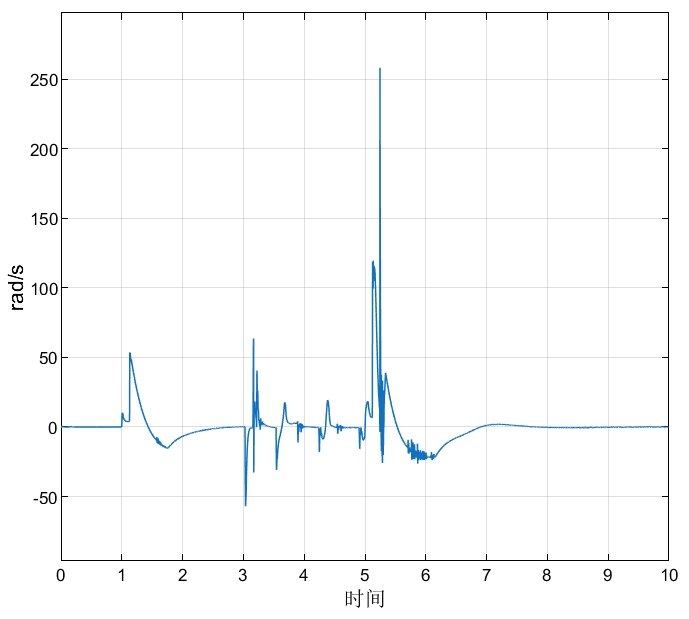
\includegraphics[width=0.5\textwidth]{figures/simulink_dtheta_b.png}
  \caption{状态量机体倾角速度变化曲线}
  \label{fig:dtheta_b}
\end{figure}
由此可见，机器人能够成功地越过障碍物，并且在整个过程中保持稳定的姿态和运动轨迹。这表明我们设计的控制方案在仿真环境中是有效的，能够实现预期的运动控制目标。

\begin{figure}[H]
  \centering
  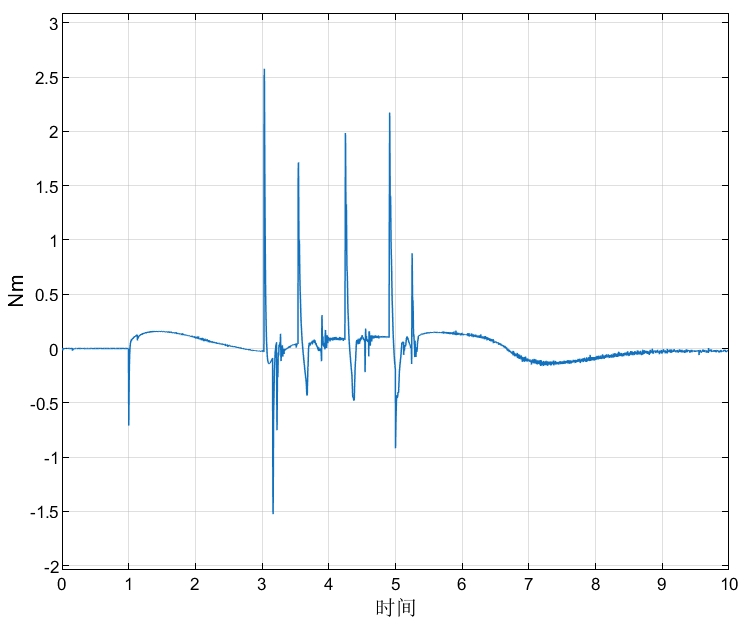
\includegraphics[width=0.7\textwidth]{figures/control_l_t.png}
  \caption{越障中的轮电机输出力矩}
  \label{fig:torque_wheel}
\end{figure}
\begin{figure}[H]
  \centering
  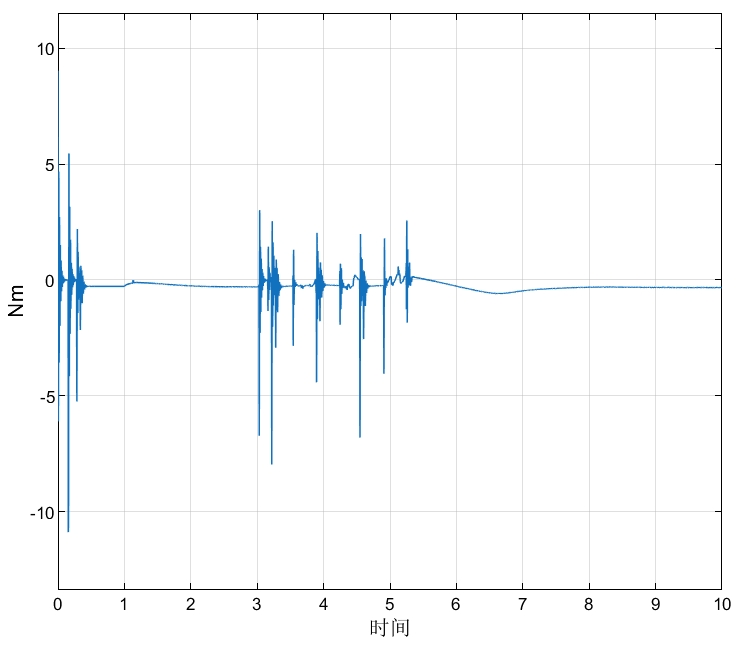
\includegraphics[width=0.7\textwidth]{figures/control_l_t1.png}
  \caption{越障中的前关节电机输出力矩}
  \label{fig:torque_joint_front}
\end{figure}
\begin{figure}[H]
  \centering
  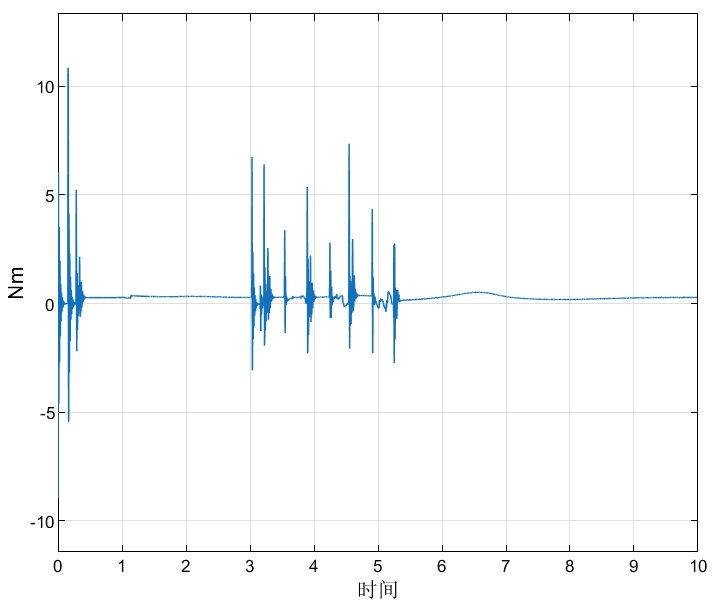
\includegraphics[width=0.7\textwidth]{figures/control_l_t4.png}
  \caption{越障中的后关节电机输出力矩}
  \label{fig:torque_joint_back}
\end{figure}

此外，我们再对越障过程中机器人的轮电机、关节电机输出进行分析，结果如图\ref{fig:torque_wheel}、\ref{fig:torque_joint_front}和\ref{fig:torque_joint_back}所示。可以看出，在越障过程中，轮电机和关节电机的输出都发生了明显的变化，以适应不同阶段的运动需求，但未达到饱和，且最终趋于稳定，这进一步验证了我们设计的控制方案能够根据环境变化动态调整控制输入，从而实现稳定的运动控制。
% <<< END INPUT chapters/10_control_simulation.tex
% >>> BEGIN INPUT chapters/11_path_planning.tex
\chapter{电缆机器人的路径规划算法}\label{chap:path_planning}

\section{路径规划目标}
电缆机器人主要工作于输电线路等复杂环境中，其路径规划的核心目标是在确保机器人自身运动稳定与安全的前提下，寻找一条从当前起点到终点的无碰撞、且在时间和能量上达到最优的可行路径，包括动态避障和静态避障和追踪目标的轨迹规划。具体而言，针对本文的五连杆轮腿式电缆机器人，路径规划目标可归纳为以下几个方面：
\begin{enumerate}
    \item 安全性与稳定性：路径规划必须确保机器人在行进过程中不会发生脱线、翻转或碰撞等危险情况。为此，规划出的路径需要满足机器人运动学和动力学的约束条件，如腿部摆角、机体俯仰角、轮子与地面接触状态等，以保证机器人在复杂地形中的稳定行进。
    \item 效率与最优性：在满足安全性的前提下，路径规划应尽可能优化行进时间和能量消耗。对于电缆机器人而言，续航能力有限，因此规划出的路径应尽量避免不必要的绕行和频繁的加速减速，以提高整体作业效率。
    \item 环境适应性：电缆机器人通常需要在未知或动态变化的环境中作业，如遇到突发障碍物、环境条件变化等情况时，路径规划算法应具备实时调整能力，能够快速重新规划路径以适应新的环境状况，确保任务的连续性和安全性。
\end{enumerate}

\section{传统路径规划算法}
在移动机器人领域，经典的传统路径规划算法主要包括基于图搜索的全局算法（如 A*、Dijkstra）、基于采样的算法（如 RRT）以及局部避障算法（如人工势场法 APF、动态窗口法 DWA）。针对电缆机器人的运行特性，这里主要介绍 A* 与 DWA 算法，并探讨它们在面对复杂动态避障时的适用性。

\subsection{A* 算法}
A* 算法是一种结合了启发式信息的经典图搜索策略，因其在静态路网中寻找最短路径时的高效性和完备性而被广泛使用。其核心思想是通过评估函数 $f(n)$ 来决定节点的扩展顺序，评估函数定义为：
\begin{equation}
    f(n) = g(n) + h(n)
\end{equation}

其中，$n$ 代表当前考察的节点；$g(n)$ 为从起点到当前节点 $n$ 的实际已花费代价；$h(n)$ 是从节点 $n$ 到终点的启发式预估代价（通常采用欧几里得距离或曼哈顿距离）。

A* 算法的具体工作流程如下：
\begin{enumerate}
    \item 初始化：建立两个列表，Open List（待考察节点集合）和 Closed List（已考察节点集合）。将起点加入 Open List。
    \item 选择节点：从 Open List 中选出评估函数 $f(n)$ 最小的节点作为当前节点 $n_c$。如果 $n_c$ 是终点，则规划完成，通过回溯指针生成最终路径。
    \item 节点扩展：将 $n_c$ 从 Open List 移入 Closed List。遍历 $n_c$ 的所有相邻可行节点，对于任意合格相邻节点 $n_a$，计算其代价值。
    \item 状态更新：若 $n_a$ 不在 Open List 中，则将其加入并记录父节点为 $n_c$；若已存在且新的路网走法下 $g(n_a)$ 更优，则更新其 $g(n_a)$ 值和父节点指向。重复上述步骤直到 Open List 为空或到达终点。
\end{enumerate}

对于电缆机器人而言，如果在作业前能提前获知整条线路上碎石等静态障碍物的绝对坐标，A* 算法能在宏观层面生成一系列无碰撞的基准跨越点。然而，A* 算法本质上是一个静态全局规划器，当传感器检测到移动的未知障碍物时，预先构建的静态栅格地图会面临大范围失效。此时若强行避让动态目标，必须进行极高频率的全局节点重置与启发式规划，这不仅计算开销庞大，更会引起不可接受的控制延迟现象。因此，A* 算法虽然在静态环境中表现优异，但在电缆机器人面临的高度动态和不确定环境中，其适用性和效率都将会受到严重限制。

\subsection{DWA 动态窗口法}
相比之下，DWA（Dynamic Window Approach）是一种常用且高效的局部实时避障算法。它将位置空间的避障问题转化为机器人的速度空间 $(v, \omega)$ 中的优化搜索问题。其核心思想在于：结合机器人的物理运动极限计算出一个安全的“速度窗口”，并在此窗口内通过轨迹推演寻找当前最优速度下发执行。

DWA 算法的速度窗口计算约束主要包含以下三个递进层次：
\begin{enumerate}
    \item 基础运动学约束 $V_m$：受限于机器人电机性能的最大/最小设计速度。该全集限定了线速度 $v \in [v_{min}, v_{max}]$ 与角速度 $\omega \in [\omega_{min}, \omega_{max}]$。
    \item 电机动态加减速约束 $V_d$：由于机器人不可能发生瞬间速度跃变，在下一次控制周期 $\Delta t$ 内，其可达到的速度窗口被严格限制在当前速度 $(v_c, \omega_c)$ 与极大加速度 $(a_v, a_\omega)$ 的物理爬升范围内：
    \begin{equation}
        V_d = \{ (v, \omega) \mid v \in [v_c - a_v \Delta t, v_c + a_v \Delta t], \omega \in [\omega_c - a_\omega \Delta t, \omega_c + a_\omega \Delta t] \}
    \end{equation}
    \item 安全刹车约束 $V_a$：为了保证机器人绝对不与雷达线上的障碍物相撞，算法要求所有入选速度必须能在其撞击前安全刹停（设雷达扫描距离为 $\text{dist}$）：
    \begin{equation}
        V_a = \left\{ (v, \omega) \mid v \le \sqrt{2 \cdot \text{dist}(v, \omega) \cdot a_v}, \;\; \omega \le \sqrt{2 \cdot \text{dist}(v, \omega) \cdot a_\omega} \right\}
    \end{equation}
\end{enumerate}

最终在每个周期内被允许采样的动态速度窗口 $V_r$ 是以上三者的交集：$V_r = V_m \cap V_d \cap V_a$。

在计算出安全域 $V_r$ 的范围后，DWA 流程会对窗口内的各个速度对 $(v, \omega)$ 离散化采样，并进行固定时长的前向模拟轨迹推演，随后通过以下评价函数对所有推演出的末端状态进行在线归一化打分求解：
\begin{equation}
    G(v, \omega) = \sigma \left( \alpha \cdot \text{heading}(v, \omega) + \beta \cdot \text{dist}(v, \omega) + \gamma \cdot \text{vel}(v, \omega) \right)
\end{equation}

其中，$\text{heading}$ 评估轨端航向角偏离目标位置的程度（越小越好）；$\text{dist}$ 用于惩罚靠近障碍物的行为并衡量安全间距；$\text{vel}$ 负责鼓励机器人保持较高的期望线速度。系统会在每一个时间步选取 $G(v, \omega)$ 得分最高的最优速度指令发送给底层电机。

\subsection{传统算法的选择结论}
对于电缆机器人的实际应用，复杂高空环境中最核心的挑战在于非线性风偏扰动和不可预知的动态移动障碍。全局静态的 A* 算法由于缺乏对突发雷达信息的自适应重规划能力，耗时且僵硬，难以真正满足实时动态主动避障的苛刻需求。而 DWA 算法得益于对底层动力学的严格窗口约束（即刻考虑最大刹车距离）和局部微秒级别时间模拟轨迹评估能力，在处理传感器即时获取的动态对象时表现出了极强的反馈式顺滑躲避优势。因此，本课题通过分析传统算法的数学原理与计算流后，决定最终摒弃 A* 算法，仅选取最优的 DWA 算法作为传统局部避障的基准对比模型，以此在后续仿真中直观对照出课题自主设计的深度强化学习网络在电网避障中的长效预测等优越性性能。

\section{强化学习路径规划算法}
针对传统基于模型与搜索算法在高维、非线性连续状态空间控制及未知动态环境中的不足，基于深度强化学习（Deep Reinforcement Learning, DRL）的路径规划为电缆机器人提供了更为先进的智能化解决思路。强化学习算法通过智能体（Agent）与环境的不断试错交互来学习最佳策略，摆脱了对精确全局地图和复杂运动学求逆的高度依赖，展现出了绝佳的泛化能力。

在具体的电缆机器人路径规划任务中，常用的连续动作空间算法包括 DDPG（深度确定性策略梯度算法）、PPO（近端策略优化算法）以及 SAC（柔性动作评价算法）等。以该五杆轮腿机器人的电缆越障及行进规划为例，其强化学习模型可进行如下抽象定义：
\begin{enumerate}
    \item 状态空间 (State)：机器人通过自身传感器与相关集体解算，包括机器人前进和转向速度、位移，左右腿角和腿角速度，机体倾角和机体倾角速度，共计10个状态量。
    \item 动作空间 (Action)：由强化学习策略网络输出的控制动作，可能为离散值也可以为连续值，作为整个机器人的前进和转向输出，可以通过lqr与vmc转换为底层电机的具体控制指令。
    \item 奖励函数 (Reward)：引导智能体进化的主要依据。其应包含对向目标点靠近并抵达的终极奖励、对产生摩擦碰撞及姿态失稳（例如翻转、力矩超限）的严厉惩罚。同时可加入控制量平滑变化的惩罚项，促使智能体策略更加节能、稳健。
    为了引导智能体（Agent）在复杂的避障环境中快速、稳定地到达目标点，本文设计了一个多维度的向量化奖励函数。该函数由稠密奖励（Dense Reward）与稀疏奖励（Sparse Reward）共同组成。
\end{enumerate}

\subsection{训练过程设计}

\begin{table}[H]
  \centering
  \caption{训练结果定义表}\label{tab:training_definition}
  \renewcommand{\arraystretch}{1.3}
    \begin{tabular}{lp{0.72\textwidth}}
    \toprule
    \textbf{信号} & \textbf{含义}  \\
    \midrule
    截断信号（$t_r$）& 当步数超过最大步数限制 $T_{max}$ 时触发  \\
        终止信号（$d_w$）& 由以下三种情况的并集触发：成功信号（$win$）：智能体与目标的距离 $d_t$ 小于目标区域半径 $d_{threshold}$；碰撞信号（$collide$）：传感器观测到的最小障碍物距离小于碰撞阈值 $d_{collision}$；出界信号（$exceed$）：智能体与目标点的距离超过了预设的最大范围 $D$。\\
    \bottomrule
  \end{tabular}
\end{table}

\subsection{奖励函数设计}

\subsubsection{稠密奖励项设计}

稠密奖励由以下四个子项加权构成。

距离进度奖励（$R_{dist}$）：
\begin{equation}
    R_{dist} = \mathrm{clamp}\left( \frac{d_{t-1} - d_t}{v_{max} \cdot \Delta t}, -1, 1 \right)
\end{equation}
该项鼓励智能体向目标点移动，靠近时获得正奖，背离时获得惩罚。

航向对齐奖励（$R_{ori}$）：
\begin{equation}
    R_{ori} = \frac{0.25 - \mathrm{clamp}(|\alpha|, 0, 0.25)}{0.25}
\end{equation}
该项在智能体正对目标点（$\alpha \approx 0$）时取得最大值 1，随着偏差增大迅速衰减至 0。

动作倾向奖励（$R_{fwd}$）：为了防止智能体在原地滞留，针对前进动作给予奖励。在连续空间下，定义为：
\begin{equation}
    R_{fwd} = \mathbb{I}(v_{linear} > 0.5)
\end{equation}

后退与减速惩罚（$R_{ret}$）：
\begin{equation}
    R_{ret} = \mathbb{I}(v_{linear} \leq 0)
\end{equation}

\subsubsection{综合奖励函数}

最终的奖励函数 $R_{total}$ 表达式如下。为了防止智能体通过原地徘徊“刷分”，引入了 $-0.5$ 的时间惩罚（Living Penalty）项：
\begin{equation}
    R_{step} = 0.5 \cdot R_{dist} + (R_{ori} \cdot R_{fwd}) - 0.5 \cdot R_{ret} - 0.5
\end{equation}

当触发终止信号时，使用稀疏奖励进行覆盖：
\begin{equation}
    R_{total} =
    \begin{cases}
        R_{AWARD} & \text{if } win = 1 \\
        R_{PUNISH} & \text{if } collide = 1 \text{ or } exceed = 1 \\
        R_{step} & \text{otherwise}
    \end{cases}
\end{equation}

\subsection{DQN}
DQN（Deep Q-Network，深度Q网络）是强化学习领域的一个标志性算法。它将深度神经网络（Deep Learning）与传统的Q-Learning相结合，有效解决了传统强化学习在处理高维、连续状态空间时遭遇的“维度灾难”问题。以下是 DQN 算法几个核心原理与机制：

\subsubsection{价值函数近似}
传统的 Q-Learning 通过维护一张 Q-Table 来记录在每个状态 $s$ 下采取动作 $a$ 对应的期望累计回报 $Q(s, a)$。但在复杂的连续环境中，状态数量可能极其庞大。DQN 提出使用一个深度神经网络（Q 网络）来近似拟合这个 Q 函数：
\begin{equation}
    Q(s, a; \theta) \approx Q^*(s, a)
\end{equation}
其中 $\theta$ 是神经网络的参数，输入为状态 $s$，输出是在该状态下各个离散动作的 $Q$ 值。

\subsubsection{经验回放}
智能体与环境交互产生的数据通常具有极强的时间相关性。如果直接使用这些序列数据训练神经网络，容易引发灾难性遗忘并导致网络极其不稳定。DQN 引入了容量为 $N$ 的经验回放池，将智能体每一步的经验元组 $(s, a, r, s')$ 存储起来。在训练网络时，从中随机抽取一个小批量数据进行梯度下降。这种机制打破了数据间的时间相关性，使其近似独立同分布，同时提高了样本的利用率。

\subsubsection{双网络结构}
在传统的 Q-Learning 中，更新当前 Q 值的 TD 目标（Temporal Difference Target）依赖于 Q 值本身。如果只用一个网络，在更新当前 Q 值的同时，目标 Q 值也会随之改变，极易导致训练震荡甚至发散。为此，DQN 采用了两个结构完全相同的神经网络：
\begin{enumerate}
    \item 评估网络（Evaluate Network） $Q(s, a; \theta)$：负责输出当前的 Q 值，并且在每一步都通过梯度下降进行参数更新。
    \item 目标网络（Target Network） $Q_{target}(s', a'; \theta^-)$：负责计算 TD 目标。其参数 $\theta^-$ 会被冻结，不参与梯度更新，仅在每隔一定步数后，将评估网络的参数 $\theta$ 完整复制给目标网络。
\end{enumerate}

该机制使得一段时间内的目标值保持相对固定，大幅提高了训练的稳定性。

\subsubsection{损失函数计算}
DQN 的本质是一个回归任务，其目标是让评估网络输出的预测值 $Q_{eval}(s, a)$ 尽可能逼近真实的目标值。其损失函数通过均方误差（MSE）定义为：
\begin{equation}
    Loss(\theta) = \mathbb{E}_{(s,a,r,s') \sim U(D)} \left[ \Big( \underbrace{r + \gamma \max_{a'} Q_{target}(s', a'; \theta^-)}_{\text{TD 目标值}} - \underbrace{Q_{eval}(s, a; \theta)}_{\text{当前预测值}} \Big)^2 \right]
\end{equation}
其中 $r$ 为即时奖励，$\gamma$ 为折扣因子。网络通过让该 Loss 最小化，利用反向传播算法（如 Adam 优化器）更新评估网络的参数 $\theta$。

\subsubsection{$\epsilon$-Greedy 策略工作流程}
为了平衡探索（尝试新动作）与利用（选择当前利益最大的动作），DQN 采用 $\epsilon$-greedy 策略：以 $\epsilon$ 的概率随机选择一个动作，以 $1 - \epsilon$ 的概率选择当前评估网络认为 $Q$ 值最大的动作 $a = \arg\max_{a} Q_{eval}(s, a; \theta)$。

整个 DQN 的工作流程如下：
\begin{enumerate}
    \item 观察当前状态 $s$；
    \item 根据 $\epsilon$-greedy 策略选择动作 $a$；
    \item 执行动作，获得奖励 $r$ 和新状态 $s'$；
    \item 存储该经验 $(s, a, r, s')$ 到经验回放池中；
    \item 从池中随机抽取一批数据；
    \item 计算 Loss 并利用梯度下降更新评估网络的参数 $\theta$；
    \item 定期将评估网络的参数同步给目标网络 $\theta^-$。
\end{enumerate}

\subsection{SAC}
SAC（Soft Actor-Critic，柔性行为者-评论家算法）是一种基于最大熵强化学习框架的算法。与传统的强化学习方法相比，SAC 通过引入熵正则化项来鼓励智能体在策略选择上保持一定程度的随机性，从而提高了探索效率和策略的鲁棒性。以下是 SAC 的核心原理与机制：

\subsubsection{最大熵目标函数}
传统的强化学习旨在寻找一个策略 $\pi$ 来最大化期望累计奖励。而在 SAC 中，目标函数被修改为最大化期望累积奖励与策略熵（Entropy）之和。其目标函数定义为：
\begin{equation}
    J(\pi) = \sum_{t=0}^{T} \mathbb{E}_{(s_t, a_t) \sim \rho_\pi} \left[ r(s_t, a_t) + \alpha \mathcal{H}(\pi(\cdot|s_t)) \right]
\end{equation}

其中，$\alpha$ 是温度参数，用于控制奖励与熵之间的相对重要性；$\mathcal{H}(\pi(\cdot|s_t))$ 是策略在状态 $s_t$ 下的香农熵。熵越大，表示智能体对动作的选择越随机。这种机制促使智能体在能够完成任务的前提下，尽可能多地探索不同的动作，从而极大地提升了算法的探索能力和对环境持续变化的鲁棒性。

\subsubsection{柔性价值函数与贝尔曼方程}
基于最大熵框架，SAC 重新定义了状态价值函数（Soft Value Function）和动作价值函数（Soft Q-Function）。柔性状态价值函数 $V(s_t)$ 包含了熵奖励：
\begin{equation}
    V(s_t) = \mathbb{E}_{a_t \sim \pi} \left[ Q(s_t, a_t) - \alpha \log \pi(a_t|s_t) \right]
\end{equation}

对应的柔性贝尔曼方程更新规则为：
\begin{equation}
    Q(s_t, a_t) = r(s_t, a_t) + \gamma \mathbb{E}_{s_{t+1} \sim p} \left[ V(s_{t+1}) \right]
\end{equation}

在实际算法实现中，SAC 通常使用神经网络来逼近这些价值函数。

\subsubsection{Actor-Critic 架构与双 Q 网络机制}
SAC 采用了 Actor-Critic（演员-评论家）架构，能够很好地处理连续动作空间：
\begin{enumerate}
    \item Critic 网络：为了缓解 Q 值的高估问题（Overestimation Bias），SAC 借鉴了 TD3 算法的思想，使用两个独立的 Q 网络 $Q_{\theta_1}$ 和 $Q_{\theta_2}$，在计算目标值时取两者的最小值：$Q_{target} = \min(Q_{\theta_1}, Q_{\theta_2})$。
    \item Actor 网络：负责输出一个随机策略。在连续控制任务中，通常假设策略服从高斯分布，Actor 网络输出该分布的均值 $\mu$ 和协方差 $\Sigma$。
\end{enumerate}

\subsubsection{重参数化技巧（Reparameterization Trick）}
由于 Actor 网络的输出是一个概率分布，直接从分布中采样动作 $a_t$ 会阻断梯度反向传播。为了解决这一问题，SAC 使用了重参数化技巧。具体而言，动作被表示为一个确定性函数 $f_\phi$ 与独立噪声 $\epsilon$ 的结合：
\begin{equation}
    a_t = f_\phi(\epsilon_t; s_t)
\end{equation}

其中噪声 $\epsilon_t$ 通常采样自标准正态分布 $\mathcal{N}(0, I)$。通过这种方式，采样过程的随机性被转移到了外部噪声上，使得 Actor 网络的参数 $\phi$ 能够通过链式法则顺利进行梯度更新。
% --- 补充 SAC 与 DQN 的对比描述 ---
\subsubsection{离散与连续动作空间的平衡}
DQN 及其变体在处理离散动作空间时表现出色，但其本质上依赖于对所有可能动作计算 $Q$ 值并取最大值（$\max$ 操作）。在面对高维甚至无限维的连续动作空间时，DQN 必须对动作空间进行离散化，但这会导致“维度灾难”并丢失精度。

相比之下，SAC 能够天然地处理连续动作空间。通过 Actor 网络输出动作分布的参数（均值与标准差），SAC 可以在连续区间内进行高效采样。此外，通过引入熵正则化，SAC 不仅解决了 DQN 容易陷入局部最优的问题，还显著提升了在复杂连续控制任务中的鲁棒性。

% --- 新增 Transformer 架构及其在 SAC 中的应用描述 ---
\subsection{Transformer 架构与时序特征建模}
在复杂的动态环境中，环境状态往往具有部分可观测性（POMDP），仅依赖当前时刻的状态 $s_t$ 难以做出最优决策。为了捕获历史观测中的长期时序依赖关系，本文引入 Transformer 架构作为 SAC 算法的状态编码层，用于串联时序信息。

\subsubsection{自注意力机制（Self-Attention）}
Transformer 的核心是多头自注意力机制（Multi-Head Self-Attention, MHSA）。它通过查询（Query）、键（Key）和值（Value）的交互，自动学习序列中不同时间步观测值之间的关联权重。对于输入序列 $X$，其注意力计算公式为：
\begin{equation}
    \text{Attention}(Q, K, V) = \text{softmax}\left(\frac{QK^T}{\sqrt{d_k}}\right)V
\end{equation}
其中 $d_k$ 是缩放因子。通过多头机制，网络可以同时从多个表示子空间学习时序特征。

\subsubsection{位置编码（Positional Encoding）}
由于自注意力机制本身不具备处理序列顺序的能力，本文引入了位置编码来赋予模型时间感知能力。通过将位置向量与状态嵌入向量相加，模型能够分辨不同时间跨度下的状态演变趋势。

\subsubsection{Transformer 与 SAC 的串联集成}
在本文设计的架构中，Transformer 充当了特征提取器。具体工作流程如下：
\begin{enumerate}
    \item 序列输入：将历史 $k$ 个时间步的状态、动作序列 $[s_{t-k}, a_{t-k}, \dots, s_t]$ 作为输入。
    \item 特征聚合：通过 Transformer Encoder 模块进行并行计算，输出高度压缩的时序上下文向量 $z_t$。
    \item 策略与价值输出：将 $z_t$ 分别输入 SAC 的 Actor 网络和双 Critic 网络。
\end{enumerate}

\begin{equation}
    \pi(a_t | s_{t-k:t}, \phi) = \text{Actor}(\text{Transformer}(s_{t-k:t}))
\end{equation}

这种“Transformer + SAC”的结构通过 Transformer 强大的表征能力解决了长时序建模问题，同时利用 SAC 的最大熵框架保证了在连续控制任务中的探索效率与稳定性。

\subsection{算法原理初步对比}
本章详细梳理了机器人在路径规划与运动控制领域的核心算法。首先，探讨了传统的经典导航框架，介绍了 A* 算法在全局路径规划中寻找启发式最优路径的原理，以及 DWA算法在局部路径规划中出色的实时动态避障机制。随后，本文将视角转向基于深度强化学习的智能控制方案，详细梳理了 DQN 与 SAC 算法的核心原理，并在此基础上探讨了引入 Transformer 架构以强化模型对长时序状态表征能力的机制。DQN 通过经验回放与双网络结构奠定了深度强化学习的基础，但在处理高维连续动作空间时存在固有局限；SAC 通过最大熵框架有效提升了连续控制任务中的探索效率与鲁棒性；而 Transformer 与 SAC 的深度融合，则进一步弥补了传统算法在处理部分可观测环境时的短板。

为了更直观地评估上述算法及其改进架构的性能差异与适用场景，本文将在后续小节中结合具体的仿真实验环境，对DWA、DQN、SAC 以及基于 Transformer 增强的 SAC 算法展开详细的对比实验与多维度结果分析。
% <<< END INPUT chapters/11_path_planning.tex
% >>> BEGIN INPUT chapters/12_path_planning_simulation.tex
\chapter{路径规划仿真试验}\label{chap:path_planning_simulation}
本章节仿真效果很多基于动画展示，不便于在论文中直接展示，相关仿真视频与源代码已上传至GitHub项目主页（\url{https://github.com/misedeshitou/ColorDynamic}）。

\section{仿真环境介绍}
本文路径规划算法的训练与测试均基于开源强化学习仿真平台 Sparrow（\url{https://github.com/XinJingHao/Sparrow-V2}）展开。Sparrow 以 Pygame 为渲染后端，在二维平面内模拟一台搭载激光雷达的差速轮式机器人，执行含动静态障碍物的点到点导航任务。其交互接口遵循标准 Gym 规范，主要包含以下三个要素：

\begin{enumerate}
    \item 观测空间：包括激光雷达的离散测距序列、机器人当前线速度与角速度，以及目标点在车体坐标系下的相对距离与航向偏角。
    \item 动作空间：智能体输出线速度与角速度指令，支持离散和连续两种模式。
    \item 任务目标：在含随机障碍物的动态场景中，以尽量短的路径无碰撞地到达目标点。
\end{enumerate}

选用 Sparrow 的主要原因在于其训练效率高、物理建模贴近实际两点。

\subsection{训练效率}

\begin{enumerate}
\item 并行环境：Sparrow 底层基于 PyTorch 实现，支持通过超参数 $N$ 同时运行多个独立环境副本。运动学积分、雷达模拟与碰撞检测均以批量矩阵运算的形式在 GPU 上执行，显著提升了单位时间内的样本采集量。
\item 零拷贝数据流：Gazebo、Webots 等传统仿真器在 CPU 端完成物理计算后，需将观测数据显式拷贝至 GPU 供网络推理，存在较大的通信开销。Sparrow 的观测张量直接在显存中生成，省去了跨设备传输步骤。
\item 域随机化：每轮 reset 时，环境随机化障碍物的数量、形状、位置及运动速度，并可在雷达读数和底盘执行层面叠加高斯噪声与控制延迟，有助于提升策略的 Sim2Real 迁移能力。
\end{enumerate}

\subsection{物理建模}

\begin{enumerate}
    \item 一阶惯性运动学：环境内置一阶低通滤波器模拟电机响应迟滞，实际速度 $V_{\text{now}}$ 的更新规则为：
    \begin{equation}
        V_{\text{now}} = K \cdot V_{\text{prev}} + (1-K) \cdot V_{\text{target}}
    \end{equation}
    即使发出较大的加减速指令，车体速度也不会瞬间跃变。本文训练时将滤波系数设为 $K=0.6$，以贴近真实电驱底盘的响应特性，同时促使策略网络学习提前减速等预判行为。
    \item 栅格化雷达模拟：传统方法通过计算几何求射线与障碍物的交点，计算量较大。Sparrow 将障碍物编码为像素栅格，以雷达中心为原点向各方向同步扩散射线，利用 GPU 并行计算每条射线的首个遮挡距离，在保证精度的同时大幅降低了计算耗时。
\end{enumerate}

\subsection{动作空间}

针对不同算法的需求，Sparrow 提供离散与连续两种动作模式。

\subsubsection{离散动作空间}

离散模式下，动作空间共包含 8 个预设指令，覆盖前进、转弯、后退及静止等基本运动基元，适用于 DQN 等仅支持离散输出的算法，具体映射关系见表~\ref{tab:discrete_action}。

\begin{table}[H]
    \centering
    \caption{离散动作索引与对应运动指令}
    \label{tab:discrete_action}
    \begin{tabular}{llcc}
        \toprule
        \textbf{动作索引} & \textbf{运动含义} & \textbf{线速度 ($v$)} & \textbf{角速度 ($\omega$)} \\
        \midrule
        0 & 左转（小半径） & $0.2\,v_{\max}$ & $+\omega_{\max}$ \\
        1 & 左转（大半径） & $v_{\max}$ & $+\omega_{\max}$ \\
        2 & 直线前进 & $v_{\max}$ & $0$ \\
        3 & 右转（大半径） & $v_{\max}$ & $-\omega_{\max}$ \\
        4 & 右转（小半径） & $0.2\,v_{\max}$ & $-\omega_{\max}$ \\
        5 & 直线后退 & $-v_{\max}$ & $0$ \\
        6 & 微速前进 & $0.1\,v_{\max}$ & $0$ \\
        7 & 原地静止 & $0$ & $0$ \\
        \bottomrule
    \end{tabular}
\end{table}

\subsubsection{连续动作空间}

连续模式下，策略网络输出二维向量 $[a_1,\,a_2]\in[-1,1]^2$，环境按固定比例尺将其映射为底盘物理量：线速度：$V_l = a_1 \times 50\,\text{cm/s}$ ；角速度：$\omega = a_2 \times 2\,\text{rad/s}$

SAC、TransSAC 等基于连续控制的算法均采用此模式。

\subsection{评估指标}
采用100次独立随机初始化的测试场景，评估算法在路径规划任务中的表现。评测指标包括：
\begin{enumerate}
    \item \texttt{ep\_steps}：平均每回合步数

    统计\texttt{total\_steps / finished}，其中到达目标用真实步数，失败/超时按 500 次计罚。

    \item \texttt{ep\_r}：平均每回合总奖励

    统计方式是 \texttt{total\_r / finished}，统计成功回合数的平均总奖励。

    \item \texttt{arrival\_rate}：到达率

    统计100次测试场景中成功回合次数，作为到达率的百分比。

    \item \texttt{total\_score}：综合总分数

    \begin{itemize}
        \item 步数分：$\texttt{normed\_ep\_steps} = (500-\texttt{ep\_steps})/(500-70)$
        \item 奖励分：$\texttt{normed\_ep\_r} = \texttt{ep\_r}/220$
        \item 综合分：$\texttt{normed\_total\_score} = (\texttt{normed\_ep\_steps} + \texttt{normed\_ep\_r} + \texttt{arrival\_rate})/3$
    \end{itemize}
\end{enumerate}

\section{DWA算法调试与局部极小值问题分析}
DWA 作为传统局部规划算法，无需训练即可部署。其控制量直接由速度空间搜索得到，优点是响应快、结构清晰，但由于决策完全依赖当前时刻的局部代价，遇到障碍物密集或目标方向变化较快的场景时，容易表现出路径抖动、转向保守以及绕行效率不高等问题。

从实现角度看，DWA 在 Sparrow 环境中的核心流程仍然遵循“采样--预测--评价--输出”的闭环机制：首先在给定的线速度和角速度范围内离散采样候选控制量，再通过短时前向推演得到若干条可行轨迹，随后结合目标距离、速度偏好与障碍物距离等代价项进行综合评分，最终输出当前步的最优运动指令。为了保证仿真中的连续性与安全性，本文对预测时域、障碍物硬约束和速度权重进行了针对性调优，使其能够在动态障碍物附近保持更稳妥的运动轨迹。

在DWA算法的仿真过程中，机器人初期表现出明显的“原地打圈”现象，且设定的碰撞急停机制未能按预期生效。通过记录与分析算法运行状态，发现该现象主要源于代价函数设计的不平衡以及参数配置的局部最优陷阱。

对于DWA经典算法，相关算法模型优化与参数调优如下：
对于一个以恒定线速度 $v$ 和角速度 $\omega$ 运动的对象，其位置随时间 $t$ 的变化可写为：
\begin{equation}
\begin{aligned}
x(t) &= x_0 + \int_{0}^{t} v \cos(\theta_0 + \omega\tau) \, \mathrm{d}\tau
= x_0 + \frac{v}{\omega}\left[\sin(\theta_0 + \omega t) - \sin(\theta_0)\right],\\
y(t) &= y_0 + \int_{0}^{t} v \sin(\theta_0 + \omega\tau) \, \mathrm{d}\tau
= y_0 - \frac{v}{\omega}\left[\cos(\theta_0 + \omega t) - \cos(\theta_0)\right].
\end{aligned}
\end{equation}

\subsection{运动模型优化}
\paragraph{原始离散运动模型（Euler Method）}
这是最基础的更新方式，假设在 $\Delta t$ 时间内速度和朝向恒定。
\begin{equation}
\begin{cases}
x_{k+1} = x_k + v_k \cos(\theta_k) \Delta t \\
y_{k+1} = y_k + v_k \sin(\theta_k) \Delta t \\
\theta_{k+1} = \theta_k + \omega_k \Delta t
\end{cases}
\end{equation}

\paragraph{改进后的积分运动模型（Exact Integration）}
该模型考虑了在 $\Delta t$ 时间内朝向角 $\theta$ 的连续变化（即圆弧运动）。
\begin{equation}
\begin{cases}
x(t) = x_0 + \frac{v}{\omega}(\sin(\theta_0 + \omega t) - \sin(\theta_0)) \\
y(t) = y_0 - \frac{v}{\omega}(\cos(\theta_0 + \omega t) - \cos(\theta_0)) \\
\theta(t) = \theta_0 + \omega t
\end{cases}
\end{equation}
\paragraph{改进模型的优势}
\begin{enumerate}
    \item 消除轨迹线性化误差：原始离散模型默认采样周期内沿直线运动；当角速度较大或采样频率较低时，圆弧会被折线近似，从而产生几何误差。积分模型给出运动学方程的解析解，可显著降低该误差。
    \item 提高定位精度与稳定性：在里程计与惯性导航中，误差会随时间累积。积分模型能降低单步预测误差，尤其在高速转弯或大角度偏转工况下可提供更准确位姿估计，从而提升滤波稳定性。
    \item 增强低频采样鲁棒性：工程实践中采样频率可能受限（如 $10\,\mathrm{Hz}$）。相较高度依赖高频采样的离散模型，积分模型在较大时间步长 $\Delta t$ 下仍能保持较高轨迹精度。
\end{enumerate}

\subsection{障碍物代价函数设计}

该模型采用负指数函数计算非碰撞区域的代价值，其数学表达式为：

\begin{equation}
Cost = e^{-\frac{d}{\sigma}}
\end{equation}

其中，$d$ 表示物体与障碍物之间的净距离（$net\_dist$），$\sigma$ 为平滑因子，通常取安全距离（$safe\_dist$）的三分之一。

这样设计有以下几点优势：
\begin{enumerate}
    \item 远距离衰减：当 $d$ 较大时，$Cost$ 趋于 $0$，表示环境对路径规划的影响极小。
    \item 近距离惩罚：随着 $d$ 的减小，$Cost$ 以指数级迅速增长，形成非线性惩罚。
    \item 边界平滑性：选取 $\sigma = \frac{safe\_dist}{3}$ 使得在 $d = safe\_dist$ 处，$Cost = e^{-3} \approx 0.049$。
    
    这种参数设计为机器人提供了一个平滑的避障过渡带，使其能够平滑地绕开障碍物，避免了硬约束带来的运动不连续性。
\end{enumerate}

\subsection{典型异常现象：“打圈”陷阱分析}

当机器人陷入“打圈”状态时，其在评估所有可行轨迹后，认为原地旋转或远离障碍物绕圈的综合代价最低。导致这一现象的核心矛盾点可归结为以下三个方面：

\begin{enumerate}
    \item 权重压制与避障过度主导：在前期的代价权重分配中，避障代价（Obstacle Cost）的“排斥力”远大于目标点代价（Goal Cost）的“吸引力”。只要前往目标点的路径上存在微小的碰撞风险，系统便会为了追求极低的避障代价，而放弃尝试穿过狭小空间，最终选择在原地保持较高转速（以满足速度评价指标），从而陷入局部最优。
    
    \item 长预测时域的负面效应：在初期配置中，轨迹预测时间被设定为 $5.1\text{ s}$。在最高 $50\text{ cm/s}$ 的线速度下，系统会评估未来长达 $2.5\text{ m}$ 的运动轨迹。在密集的障碍环境中，如此长的预测轨迹在转弯时产生的“扫掠面积”极大，极易与障碍物发生干涉。为使这 $5.1\text{ s}$ 的轨迹不触碰任何障碍物，系统被迫选择曲率极大（即原地打转）的极短安全轨迹。
    
    \item 航向角代价的缺失考量：原始算法评价指标仅依赖轨迹末端至目标点的欧氏距离。当机器人背离目标时，为使终点靠近目标，系统可能生成倒车或大半径圆弧轨迹。由于缺乏对机身朝向目标点的显式约束，机器人在旋转过程中失去了强指向性，进一步加剧了原地绕圈的发生概率。
\end{enumerate}

\subsection{动态避障策略与参数调优}

针对上述局部极小值与动态避障失效问题，经过多轮实车与仿真调试，本文对DWA算法进行了如下优化:

\subsubsection{预测时间与灵敏度的权衡}
将预测时间由 $5.1\text{ s}$ 大幅下调至 $1.0\text{ s}$，并同步降低了碰撞判断的距离阈值。该调整有效减小了轨迹的扫掠面积，提高了系统对环境的响应灵敏度。需要指出的是，预测时间不宜过小，否则会导致系统“短视”，仅在临近碰撞时才产生高代价值，从而因制动距离不足而发生实际碰撞。

\subsubsection{动静态障碍物的差异化处理机制}
实验结果表明，传统的“遇障即停”逻辑在面对动态障碍物时表现不佳，极易导致机器人陷入停滞。为此，系统舍弃了全局急停机制，转而要求机器人在动态环境中保持连续的运动能力以实现主动规避。

针对静态障碍物，为提高机器人的谨慎程度，本文采用了一种在临近区域内强制拉高代价值的硬约束策略。具体而言，当障碍物净距离 $net\_dist$ 小于等于 $15.0\text{ cm}$ 时，赋予其极高的惩罚值：
\begin{equation}
norm\_obs\_cost[net\_dist \le 15.0] = 5.0
\end{equation}

在调试中发现，若该硬性惩罚值设置过高（即梯度过大），会导致各条可行轨迹的代价差异被抹平，机器人更易倾向于停滞。因此，本文将该区域惩罚值设定为与总代价函数最大值相当的水平，且仅对静态障碍物生效，从而在保证安全性的同时维持了路径规划的平滑性。此外，考虑到引入航向角代价会大幅增加参数空间的耦合度与调优复杂度，本系统最终舍弃了该指标。

经过上述策略的优化，机器人成功实现了鲁棒的动态避障功能。最终确定的DWA核心运动学限制与代价权重参数如表 \ref{tab:dwa_params} 所示。

\begin{table}[H]
    \centering
    \caption{DWA算法核心参数优化配置表}
    \label{tab:dwa_params}
    \begin{tabular}{llc}
        \toprule
        \textbf{参数变量名} & \textbf{物理意义} & \textbf{设定值} \\
        \midrule
        $max\_speed$ & 最大线速度 & $50.0 \text{ cm/s}$ \\
        $min\_speed$ & 最小线速度 & $-50.0 \text{ cm/s}$ \\
        $max\_yawrate$ & 最大角速度 & $2.0 \text{ rad/s}$ \\
        $max\_accel$ & 最大线加速度 & $2.0 \text{ m/s}^2$ \\
        $max\_dyawrate$ & 最大角加速度 & $2.0 \text{ rad/s}^2$ \\
        $v\_reso$ & 线速度搜索分辨率 & $0.1 \text{ m/s}$ \\
        $yawrate\_reso$ & 角速度搜索分辨率 & $0.2 \text{ rad/s}$ \\
        $dt$ & 控制采样周期 & $0.1 \text{ s}$ \\
        $predict\_time$ & 轨迹预测时域 & $1.0 \text{ s}$ \\
        $goal\_cost\_gain$ & 目标距离代价权重 & $0.6$ \\
        $speed\_cost\_gain$ & 期望速度代价权重 & $0.1$ \\
        $obstacle\_cost\_gain$ & 障碍物距离代价权重 & $0.3$ \\
        $robot\_radius$ & 机器人膨胀半径 & $5.0 \text{ cm}$ \\
        $safe\_dist$ & 避障预警半径 & $20.0 \text{ cm}$ \\
        \bottomrule
    \end{tabular}
\end{table}

\subsection{DWA算法评估分析}
经过上述优化，DWA 在测试集上的表现如下：

\begin{table}[H]
    \centering
    \caption{DWA经典算法测试结果}
    \label{tab:dwa_eval_result_1}
    \begin{tabular}{lcccc}
        \toprule
        \textbf{Index} & \textbf{Total Score} & \textbf{Arrival Score} & \textbf{Step Score} & \textbf{Reward Score} \\
        \midrule
        DWA & 0.304 & 0.53 & 0.442 & -0.06 \\
        \bottomrule
    \end{tabular}
\end{table}

DWA 算法的到达率（Arrival Score）仅为 0.53，意味着智能体在近一半的测试回合中未能成功导航至目标点。相比于基于深度强化学习的算法（如 SAC 等通常能达到 0.85 以上的到达率），DWA 在面对当前环境时显得较为乏力，极易发生碰撞或超时失败。

算法的总分（Total Score）仅有 0.304，且奖励得分（Reward Score）呈现负值（-0.06）。负的奖励得分说明 DWA 在导航过程中频繁触发了环境设定的惩罚条件（例如过于靠近障碍物、发生轻微剐蹭或未能在规定步数内完成任务）。同时，0.442 的步数得分（Step Score）也侧面反映出，即使 DWA 偶尔能到达终点，其规划出的路径也往往是次优的，存在大量冗余的转向与绕路。

DWA 算法表现欠佳的主要原因在于其固有的“短视”特性。作为一种基于运动学模型的局部规划器，DWA 主要依赖当前帧的传感器数据，在速度空间内通过固定的评价函数来搜索最优指令。

综上所述，DWA 算法的测试结果证明了：在具有高动态性或复杂约束的导航场景中，传统的无学习能力的局部规划算法已难以胜任。这不仅凸显了引入高级感知与长序列决策机制的必要性，也为本课题后续采用的深度强化学习算法提供了坚实的对比基石与合理性支撑。

\section{DQN算法调试}
\subsection{DQN算法实现与离散动作训练}

与 DWA 的显式代价搜索不同，DQN 通过将状态输入映射到离散动作的 Q 值分布，学习“在当前状态下应该执行哪一种动作”的策略近似，因此更适合验证奖励设计和环境建模是否合理。本文将机器人的运动命令抽象为有限个预设动作，使其能够覆盖前进、转向、后退与停止等基本控制模式，从而与环境交互形成可训练的离散决策闭环。

在训练过程中，DQN 主要依赖经验回放池和目标网络来稳定优化：一方面，经验回放打破连续采样带来的时间相关性，提高了样本利用率；另一方面，目标网络降低了 TD 目标频繁抖动造成的训练震荡，使训练过程更易收敛。由于路径规划任务中的奖励往往具有稀疏性，本文在 DQN 训练中进一步强化了进度奖励和终局奖励的区分，使智能体能够更早感知“靠近目标”和“远离障碍”的差异，避免陷入无意义的局部徘徊。

\subsection{复合引导奖励函数设计}
强化学习中，如果只有最后到达终点才给奖励（稀疏奖励），Agent 很难学习。因此需要设计密集奖励来逐步引导策略。本文采用三类引导项：

\begin{table}[H]
    \centering
    \caption{复合引导奖励函数设计}
    \label{tab:reward_design}
    \begin{tabular}{p{0.25\textwidth}p{0.43\textwidth}p{0.24\textwidth}}
        \toprule
        \textbf{奖励项} & \textbf{方法} & \textbf{目的} \\
        \midrule
        进度 / 距离奖励，$R_{\mathrm{distance}}$  & 使用差分法计算 $\Delta d = d_{t-1} - d_t$，再除以 $v_{\max} \times \Delta t$ 并截断到 $[-1,1]$ 区间进行归一化。 & 鼓励 Agent 向目标移动，靠近目标得正分，远离扣分。 \\
        姿态 / 朝向奖励，$R_{\mathrm{forward}}$  & 计算车头朝向与“车体到目标连线”间的夹角 $\alpha$；当 $|\alpha|\in[0,0.25]$ 时给予最高 1 的朝向奖励。 & 引导机器人在靠近目标的同时保持朝向正确。 \\
        动作与动力学偏好, $R_{\mathrm{retreat\_slowdown}}$ & 根据智能体输出的线速度判断其为前进、后退或减速。 & 符合物理直觉，鼓励车辆保持合理前进速度，惩罚倒车或过慢行驶。 \\
        \bottomrule
    \end{tabular}
\end{table}

奖励的组合方式为：

\begin{equation}
    \texttt{self.reward\_vec} = 0.5 \times R_{\mathrm{distance}} + R_{\mathrm{orientation}} \times R_{\mathrm{forward}} - 0.5 \times R_{\mathrm{retreat\_slowdown}} - 0.5
\end{equation}

其中，$R_{\mathrm{orientation}} \times R_{\mathrm{forward}}$ 表示只有在前进的前提下，朝向正确才有奖励；若倒车，则无法从朝向项中获益。末尾的 $-0.5$ 是时间惩罚，使每一步都有代价，从而逼迫 Agent 尽快结束回合，避免原地徘徊刷分。

终局状态需要覆盖当前步的引导奖励：到达目标时直接将奖励赋予 \texttt{AWARD}（$+100$），碰撞或越界时直接将奖励赋予 \texttt{PUNISH}（$-100$）。这样明确标记成功与失败确保 Agent 以最终成败为优先目标。

\subsection{DQN算法评估分析}
经过 5000 万步的训练，DQN 在测试集上的表现如下：

\begin{figure}[H]
  \centering
  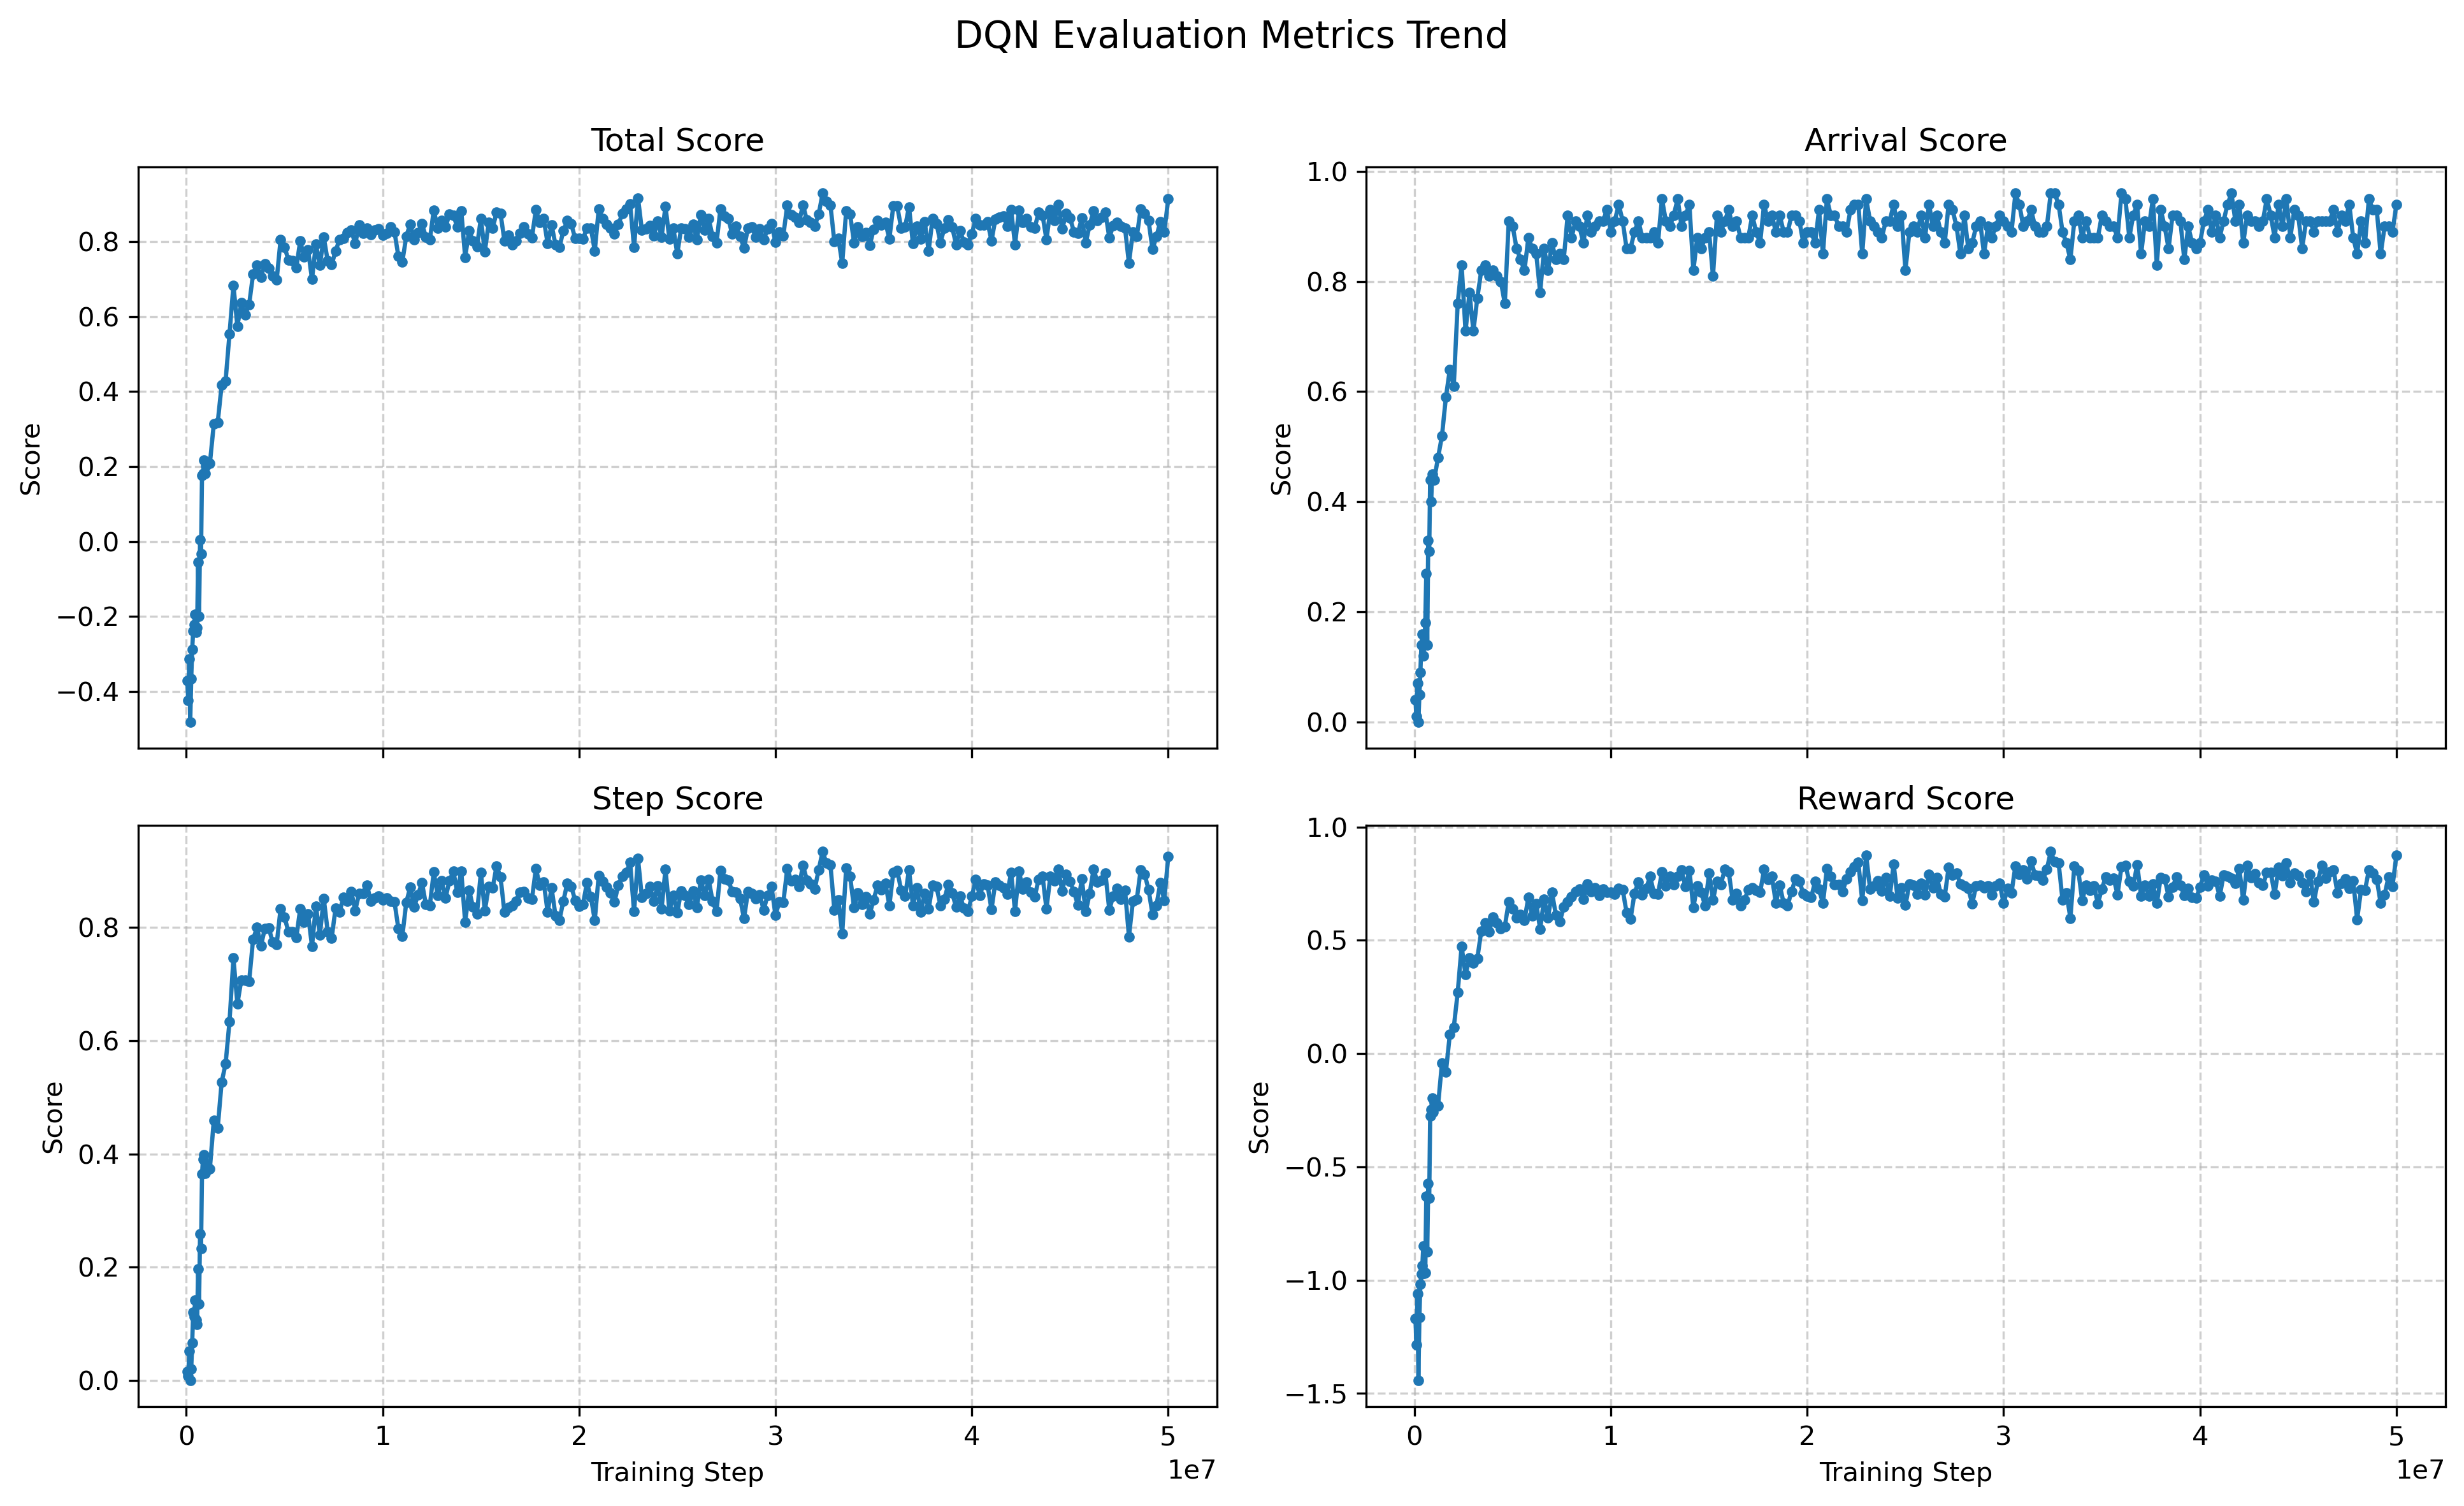
\includegraphics[width=0.7\textwidth]{figures/DQN_metrics_trend.png}
  \caption{DQN算法到达率、平均每回合步数和平均每回合奖励的训练趋势展示}
  \label{fig:dqn-showcase}
\end{figure}

从结果上看，DQN 在训练初期的探索波动相对明显，但由于离散动作空间的约束，整体收敛过程较为平稳，适合作为与连续控制算法对比的基础模型。其不足也较为直观：离散化动作会限制轨迹平滑性，机器人在转向和减速时难以形成更细粒度的控制，因此在复杂场景中的最终路径质量通常不及连续动作算法。

在训练初期（约 $0$ 至 $0.5 \times 10^7$ 步），各项指标均呈现出明显的爆发式增长。这表明智能体（Agent）在经验回放机制（Experience Replay）的作用下，能够迅速从随机探索中学习到有效策略。在 $1 \times 10^7$ 步之后，曲线进入平稳期，总分（Total Score）稳定在 0.8 左右，到达率（Arrival Score）稳定在 0.9 左右，证明算法具备良好的收敛性。

综合四项指标来看，DQN 算法在该任务场景下表现优异。步数得分（Step Score）与总分的高度一致性暗示了智能体在保证成功率的同时，也在不断优化路径或决策序列的效率。实验结果表明，所设计的奖励函数与状态空间能够引导模型学习到最优策略。

\section{SAC算法调试与ASL框架接入}
\subsection{SAC算法实现与连续动作训练}
与 DQN 相比，SAC 直接输出连续的线速度与角速度，更适合描述机器人在路径规划中的真实运动学约束，也更容易得到平滑自然的行驶轨迹。本文采用 Actor-Critic 结构对策略和价值函数进行联合建模，其中 Actor 负责给出随机策略分布，Critic 则通过双 Q 网络对动作质量进行估计，从而缓解 Q 值高估带来的训练偏差。

在工程实现上，SAC 的训练流程与本文引入的 ASL（Actor-Learner-Sharer）框架高度适配。Actor 侧持续与环境交互并向共享经验池写入轨迹数据，Learner 则从经验池中批量采样并执行参数更新，这种解耦方式有效减少了采样与训练之间的相互阻塞，提高了系统吞吐量。对于路径规划任务而言，这一结构的实际意义在于：机器人可以在高频交互中持续积累有效样本，而网络更新则在后台稳定进行，最终形成更高的样本利用效率和更平滑的收敛曲线。

调试过程中，SAC 的主要问题集中在探索阶段的随机性偏强，以及熵系数和更新节奏对收敛速度的敏感性。为此，本文在训练中对动作幅值、奖励尺度以及更新频率进行了统一约束，使策略在前期保持足够探索、后期逐步转入稳定利用。整体来看，SAC 相比 DQN 在连续控制精度和路径平滑性上具有更明显的优势，是本文后续引入 Transformer 时采用的基础骨架。

但由于SAC 训练相对于DQN所需训练时间更长，训练效率受限于单进程的采样与更新模式，本文在后续章节中引入了 ASL 分布式训练架构，以实现更高效的并行加速。

\subsection{分布式训练架构设计--Actor-Learner-Sharer模型}
\label{sec:shared_data_module}

\subsubsection{模块设计背景与目标}

在传统的单进程强化学习算法中，环境交互（数据采样）与神经网络更新（梯度下降）通常是串行执行的。这种同步阻塞的模式导致底层硬件算力无法得到充分利用，极大限制了算法的采样效率与收敛速度。因此需要分布式训练架构来解耦数据采集与模型训练的物理进程，从而实现真正意义上的并行加速。

\begin{tikzpicture}[
    % 定义通用样式
    task/.style={rectangle, draw=black, fill=blue!40, minimum width=2.5cm, minimum height=0.8cm, align=center},
    subtask/.style={rectangle, draw=black, fill=blue!40, minimum width=1.4cm, minimum height=0.6cm, align=center},
    cnode/.style={rectangle, draw=black, dashed, fill=gray!10, rounded corners=2pt, minimum width=2.5cm, minimum height=1.2cm, align=center},
    output/.style={rectangle, draw=black, fill=green!40!lime!60, minimum width=2.5cm, minimum height=0.6cm, align=center},
    % 定义箭头样式
    myarrow/.style={-{Stealth[scale=1.2]}, line width=3pt, draw=blue!40!gray}
]

% ====================
% (a) 单计算节点
% ====================
\node[task] (taskA) {任务};
\node[cnode, below=1cm of taskA] (nodeA) {计算节点};
\node[output, below=1cm of nodeA] (outA) {输出};

\draw[myarrow] (taskA) -- (nodeA);
\draw[myarrow] (nodeA) -- (outA);

\node[below=0.3cm of outA, font=\sffamily] {(a) 单计算节点};


% ====================
% (b) 分布式多计算节点
% ====================
\begin{scope}[xshift=8cm] % 将右侧图形整体向右平移
    
    % 上层：子任务
    \node[subtask] (sub2) {子任务2};
    \node[subtask, left=0.1cm of sub2] (sub1) {子任务1};
    \node[subtask, right=0.1cm of sub2] (sub3) {子任务3};

    % 中层：计算节点
    \node[cnode, below=1cm of sub2] (node2) {计算节点2};
    \node[cnode, left=0.3cm of node2] (node1) {计算节点1};
    \node[cnode, right=0.3cm of node2] (node3) {计算节点3};

    % 下层：输出
    \node[output, below=1cm of node2, minimum width=3cm] (outB) {输出};

    % 绘制连线
    \draw[myarrow] (sub1.south) -- (node1.north);
    \draw[myarrow] (sub2.south) -- (node2.north);
    \draw[myarrow] (sub3.south) -- (node3.north);

    \draw[myarrow] (node1.south) -- (outB.north west);
    \draw[myarrow] (node2.south) -- (outB.north);
    \draw[myarrow] (node3.south) -- (outB.north east);

    \node[below=0.3cm of outB, font=\sffamily] {(b) 分布式多计算节点};

\end{scope}

\end{tikzpicture}

为解决上述计算瓶颈与资源闲置问题，本研究引入 Actor–Learner 分布式训练架构，将环境交互（数据采样）与模型更新（参数学习）在物理进程上深度解耦，以打破算力瓶颈，大幅提高资源利用率与训练吞吐量。该架构主要包含以下三个核心部分：

\begin{enumerate}
\item Actor（采样器）：负责与环境进行高频交互，执行当前策略以采集经验轨迹，单步转移数据通常记录为 $(s_t, a_t, r_t, s_{t+1})$。由于仿真环境推演与逻辑判断属 CPU 密集型任务，Actor 可并行部署为大量独立进程或容器。各实例在独立的仿真环境中运行，并将采集到的数据异步写入中心经验池或以流式方式发送至 Learner。

\item Learner（学习器）：专注于神经网络参数的优化。Learner 从经验池中抽取小批量（Mini-batch）数据，并基于相应的损失函数（如 SAC 的 Actor-Critic 损失或 DQN 的 TD error）执行反向传播。作为 GPU/TPU 密集型任务，Learner 独占加速硬件资源，无需等待环境交互的物理步时延，从而实现极高的样本处理效率与梯度更新速率。

\item Sharer（参数分发器）：在大规模集群部署中常独立为参数服务组件。其主要负责全局网络权重的版本管理与分发，旨在缓解海量 Actor 同步拉取最新参数时对 Learner 计算及网络带宽造成的 I/O 瓶颈。通过高效的参数同步，Sharer 确保各 Actor 部署的策略不至于过度陈旧，严格控制 Off-policy 算法中的分布偏差。
\end{enumerate}

\subsubsection{共享数据中枢设计}
为实现跨进程及异构硬件（CPU 与 GPU）间的高效协同，本节参考 ColorDynamic 导航系统中的相关工作 \cite{colordynamic}，设计并实现了一个高性能的共享数据中枢模块（\texttt{Shared Data Module}）。该模块扮演了连接数据采集端与模型训练端的“中央物流中枢”角色。为了彻底消除高频通信带来的 I/O 瓶颈，本系统将该模块直接部署于主内存（RAM）中，利用共享内存机制实现进程间的极速交互。该模块主要承担两大核心职能：
\begin{enumerate}
    \item 构建高速数据管道：无阻塞地接收多 Actor 的并发经验写入，同时为 Learner 的高速迭代提供高吞吐量的随机批次采样（Batch Sampling）。
    \item 实现异步状态同步：作为策略网络（Policy Network）参数的高速寄存器，精准协调 Learner 完成梯度更新后的参数异步下发，以及 Actor 开启新回合前的参数非阻塞拉取。
\end{enumerate}

共享数据模块扮演了连接数据采集端与模型训练端的“中央物流中枢”角色。为了消除 I/O 瓶颈，本系统将该模块部署于主内存（RAM）中，利用共享内存机制实现进程间的极速通信。

本模块的数据流转架构如图 \ref{fig:shared_data_arch} 所示：

\begin{figure}[H]
    \centering
\begin{tikzpicture}[
    % ==== 定义通用样式 ====
    % 基础节点样式
    basebox/.style={
        rectangle, draw=black!60, thick, rounded corners=6pt, 
        align=center, minimum height=1.8cm, text=black,
        drop shadow={opacity=0.15, shadow xshift=1.5mm, shadow yshift=-1.5mm}
    },
    % 特定节点样式（带微渐变）
    buffer/.style={basebox, top color=blue!5, bottom color=blue!15, minimum width=4.8cm},
    register/.style={basebox, top color=orange!5, bottom color=orange!15, minimum width=4.8cm},
    actorbox/.style={basebox, top color=green!5, bottom color=green!15, minimum width=5cm},
    learnerbox/.style={basebox, top color=red!5, bottom color=red!15, minimum width=5cm},
    % 箭头样式
    data_arrow/.style={-{Stealth[scale=1.2]}, line width=1.5pt, draw=blue!70!gray, text=black!80},
    weight_arrow/.style={-{Stealth[scale=1.2]}, line width=1.5pt, draw=orange!80!red, text=black!80},
    % 共享内存背景样式
    shared_mem/.style={
        rectangle, draw=black!40, dashed, thick, rounded corners=10pt, 
        fill=gray!8, inner sep=18pt
    }
]

% ==== 1. 定义顶部节点 (Shared Memory 内部) ====
\node[buffer] (buffer) {
    \textbf{向量化环形经验池} \\
    \fontsize{9pt}{10pt}\selectfont \sffamily (Ring Replay Buffer) \\
    \vspace{2pt}
    \fontsize{8pt}{9pt}\selectfont \ttfamily \color{black!70} [s, a, r, s', dw] \sffamily 异构张量存储
};

\node[register, right=2.5cm of buffer] (register) {
    \textbf{模型参数寄存器} \\
    \fontsize{9pt}{10pt}\selectfont \sffamily (Actor Policy Weights) \\
    \vspace{2pt}
    \fontsize{8pt}{9pt}\selectfont \ttfamily \color{black!70} [actor\_param] \sffamily 字典状态字典
};

% ==== 2. 绘制共享数据中枢背景框 ====
\begin{scope}[on background layer]
    \node[shared_mem, fit=(buffer) (register)] (shared) {};
    % 背景框的标题
    \node[anchor=south, font=\bfseries\sffamily\large, text=black!80, yshift=4pt] 
        at (shared.north) {Shared Data 通信中枢 (主内存 RAM)};
\end{scope}

% ==== 3. 定义底部节点 ====
\node[actorbox, below=3.5cm of buffer] (actor) {
    \textbf{Actor 进程} \small (数据采集端) \\
    \vspace{2pt}
    \fontsize{9pt}{10pt}\selectfont \sffamily \color{black!70} (运行于 CPU 或 推理 GPU)
};

\node[learnerbox, below=3.5cm of register] (learner) {
    \textbf{Learner 进程} \small (模型训练端) \\
    \vspace{2pt}
    \fontsize{9pt}{10pt}\selectfont \sffamily \color{black!70} (运行于 高性能 GPU)
};

% ==== 4. 绘制数据流转箭头 ====

% (1) Actor -> Buffer (写入经验)
\draw[data_arrow] (actor.north) -- (buffer.south) 
    node[midway, left=4pt, font=\sffamily\small] {写入转移经验};

% (2) Learner -> Register (更新权重)
\draw[weight_arrow] (learner.north) -- (register.south) 
    node[midway, right=4pt, font=\sffamily\small] {更新权重};

% (3) Buffer -> Learner (采样批次数据 - 交叉线)
% 使用 pos 参数调整文字位置，并添加白色背景避免线条穿过文字
\draw[data_arrow] (buffer.315) -- (learner.135) 
    node[pos=0.25, right=4pt, font=\sffamily\small, fill=white, inner sep=2pt, rounded corners=2pt] {采样批次数据};

% (4) Register -> Actor (拉取最新权重 - 交叉线)
\draw[weight_arrow] (register.225) -- (actor.45) 
    node[pos=0.25, left=4pt, font=\sffamily\small, fill=white, inner sep=2pt, rounded corners=2pt] {拉取最新权重};

\end{tikzpicture}
\caption{分布式 Actor-Learner 共享数据流转架构图}
\label{fig:shared_data_arch}
\end{figure}

\subsubsection{核心数据结构设计}

为充分满足大规模分布式强化学习中的并发读写与异构设备协同需求，本模块在底层数据结构设计上遵循以下两项核心原则：（1）向量化存储以适应并行采样；（2）异构设备感知的透明映射以消除数据流转的物理瓶颈。

\paragraph{向量化环形缓存池（Vectorized Ring Buffer）}

在本架构中，Actor 端并行部署 $N$ 个独立的仿真环境进行同步采样。若采用传统二维经验池 $(Max\_Size, Feature\_Dim)$，则需对 $N$ 个环境的数据依次拼接后写入，这会引入高频的列表操作与内存重排开销。为此，本模块将经验回放池升级为三维张量结构 $\mathcal{D} \in \mathbb{R}^{Max\_Size \times N \times State\_Dim}$，使得 $N$ 个环境的采样数据可在底层以矩阵块的形式原子写入，避免了序列化与重新索引的计算浪费。

同时，为防止内存占用的无限增长，该缓存池采用环形覆盖机制。系统维护一个循环写入指针 $ptr$，每当新数据写入时自动递增；当 $ptr$ 达到 $Max\_Size$ 时通过取模运算 $ptr \leftarrow ptr \bmod Max\_Size$ 自动回卷至缓存起始位置，新样本覆盖最旧的数据。这一设计既保证了数据的"热"性（确保 Learner 采样自相对新鲜的转移），又严格将内存峰值锁定在预分配的上界，避免了动态扩展带来的GC延迟。

\paragraph{三端异构硬件自适应映射（Tri-Device Memory Mapping）}

在实际部署中，数据流通涉及三类计算设备：Actor 端推理设备（CPU 或推理 GPU，记为 $A\_dvc$）、中心存储设备（主内存 RAM，记为 $B\_dvc$）、Learner 端训练设备（高性能 GPU，记为 $L\_dvc$）。若在数据入库与采样的每个环节都手动管理这些设备间的张量转移，会引入繁冗的代码耦合与难以预测的内存碎片化。

为此，本模块在初始化时显式配置这三类设备标识，在执行 $\texttt{Add}()$ 与 $\texttt{Sample}()$ 等核心操作时自动调用 PyTorch 的设备无关接口（如 $\texttt{.to}(device)$）。具体地，当 Learner 调用 $\texttt{Sample}()$ 方法时，系统先从主内存批量读取数据，随后在返回前自动将其转移至 $L\_dvc$，使调用方无需感知底层的设备寻址细节。

\begin{algorithm}
\caption{共享数据中枢的异构张量流转与自旋锁控制伪代码}
\label{alg:shared_data}
\textbf{输入}: 采集端设备 $A\_dvc$ (CPU), 训练端设备 $L\_dvc$ (GPU), 经验池容量 $Max\_Size$, 批次大小 $B$\\
\textbf{初始化}: 
\begin{itemize}
    \vspace{-0.2cm}
    \item 预分配主存 ($RAM$) 经验池张量 $\mathcal{D} \in \mathbb{R}^{Max\_Size \times N \times State\_Dim}$
    \item 初始化自旋锁状态矩阵 $busy \leftarrow [\text{False}, \text{False}]$
    \item 队列写入指针 $ptr \leftarrow 0$
\end{itemize}
\vspace{-0.2cm}
\begin{algorithmic}[1]
\Function{Add}{$transition\_data$} \Comment{由 Actor 并发调用，位于 $A\_dvc$}
    \While{$busy[1] == \text{True}$} \Comment{轻量级自旋锁等待}
        \State \text{Pass} 
    \EndWhile
    \State $busy[1] \leftarrow \text{True}$ \Comment{获取经验池锁}
    \State $\mathcal{D}[ptr] \leftarrow transition\_data$ \Comment{数据存入主内存}
    \State $ptr \leftarrow (ptr + 1) \pmod{Max\_Size}$ \Comment{环形队列覆写机制}
    \State $busy[1] \leftarrow \text{False}$ \Comment{释放锁}
\EndFunction

\State
\Function{Sample}{} \Comment{由 Learner 高频调用，意图用于 $L\_dvc$}
    \While{$busy[1] == \text{True}$} 
        \State \text{Pass} 
    \EndWhile
    \State $busy[1] \leftarrow \text{True}$
    \State $batch \leftarrow \text{RandomSelect}(\mathcal{D}, B)$ \Comment{从主内存抽取小批量数据}
    \State $busy[1] \leftarrow \text{False}$
    
    \State $batch\_L \leftarrow batch\mathbf{.to}(L\_dvc)$ \Comment{\textbf{底层隐式设备映射}}
    \State \Return $batch\_L$ \Comment{返回的张量已原生驻留于 GPU}
\EndFunction
\end{algorithmic}
\end{algorithm}

\subsubsection{并发控制与轻量级读写锁机制}

在多进程共享内存架构中，并发访问冲突是系统性能的关键制约。若 Learner 在执行参数寄存器写操作时，某个 Actor 同时尝试读取该参数，将导致张量内存被破坏。更严重的是，如果采用传统的全局互斥锁（Mutex），会强制所有竞争线程进入阻塞态并触发昂贵的内核态上下文切换，这对纳秒级别的张量访问操作而言开销巨大。

针对此问题，本系统设计了细粒度自旋锁机制以替代系统级锁。核心思想是：维护一个状态向量 $\texttt{busy} \in \{\text{False}, \text{False}\}$，其中 $\texttt{busy}[0]$ 保护"模型参数寄存器"的读写，$\texttt{busy}[1]$ 保护"经验池"的读写。这种细粒度分离使得数据域与权重域的竞争可以独立控制，大幅降低了全局锁阻塞的概率。

更重要的是，当某进程发现目标锁已被占用时，不是挂起等待（开销 $\sim 100\,\mu s$），而是进入紧密自旋轮询状态（轮询周期 $\sim 10^{-4}\,s$）。鉴于张量操作通常耗时极短（$< 1\,ms$），短期轮询的开销远小于线程被唤醒的延迟，从而实现"busy-waiting 优于阻塞等待"的场景。同时，虽然自旋会消耗 CPU 周期，但由于 Learner 与 Actor 运行于不同物理核心，这种消耗不会竞争 GPU 计算资源，反而能充分利用多核的计算平面。

当双端进程竞争同一把锁（例如 Actor 和 Learner 同时尝试访问经验池）时，自旋锁机制使未获取锁的进程进入 \texttt{while True} 的高频轮询状态（休眠 $10^{-4}$ 秒级别），而非挂起等待。由于张量转移操作耗时极短，这种短效轮询机制在保证绝对数据安全的同时，将等待开销降到了最低。

\begin{figure}[H]
  \centering
  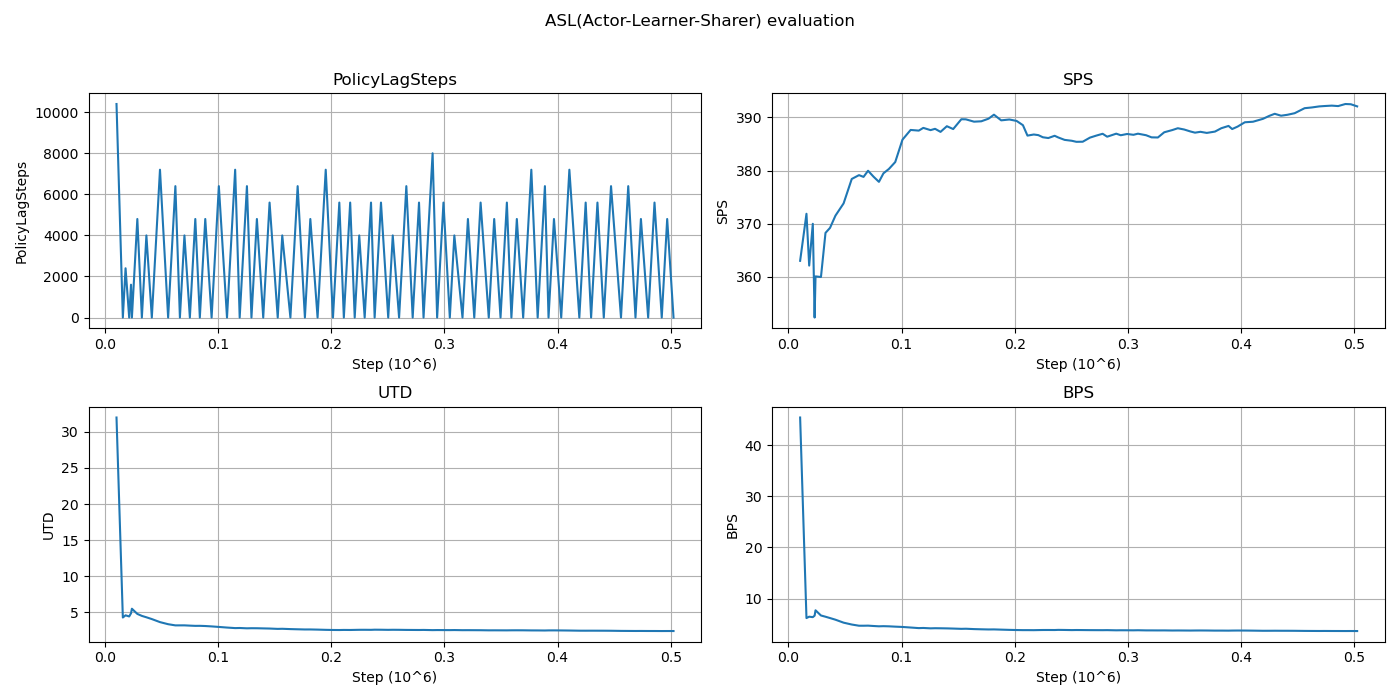
\includegraphics[width=0.9\textwidth]{figures/ASL_analysis.png}
  \caption{ASL架构性能分析}
  \label{fig:ASL-analysis}
\end{figure}
在分布式强化学习训练中，系统吞吐量、资源利用率与组件通信延迟是评估架构有效性的核心指标。图\ref{fig:ASL-analysis}给出了 Actor-Learner-Sharer（ASL）架构在 50 万步（$0.5 \times 10^6$ steps）训练周期内的性能曲线。结合曲线形态，可归纳为以下三点：
\begin{enumerate}
    \item 高效且解耦的并发吞吐量 (SPS \& BPS 分析)：
    
    ASL 架构的核心优势在于通过 Sharer（共享经验池）将数据采样（Actor）与梯度计算（Learner）进行物理与逻辑上的解耦。

    数据采样率 (SPS - Steps Per Second): 图中 SPS 曲线在训练初期经历短暂的预热后，迅速攀升并稳定在 380 至 390 之间。这表明 Actor 进程组能够以极高的效率持续与环境进行交互。SPS 的稳步微升进一步证明了环境重置或缓存机制在长期运行中表现出良好的鲁棒性，未出现阻塞或内存泄漏等衰减现象。

    批处理更新率 (BPS - Batches Per Second): Learner 的 BPS 曲线在训练极早期（探索期）处于高位，随后迅速下降并稳定在 4 左右的水平。SPS 与 BPS 的独立稳定运行，有力证明了 ASL 架构成功打破了传统单进程 RL 中“采样等训练，训练等采样”的同步木桶效应，实现了 CPU（环境推理）与 GPU（梯度反向传播）算力的满载流水线作业。

    \item 稳定的数据更新比 (UTD 分析)
    
    UTD (Update-To-Data Ratio) 定义了网络更新次数与环境交互步数的比例，是控制强化学习训练节奏的关键超参数。

    如图所示，UTD 曲线的形态与 BPS 高度一致，在经过初始的陡降后，长程稳定在较低的数值区间（约 2 至 3 左右）。这种低且稳定的 UTD 设定是针对异策略（Off-policy）算法（如 SAC）的典型优良特征。它保证了 Learner 不会因为过度消费旧数据而导致过拟合（Overfitting）或 Q 值高估，同时 Actor 源源不断地注入高新鲜度的数据，维持了探索与利用（Exploration vs. Exploitation）的动态平衡。

    \item 异步通信与容忍延迟 (PolicyLagSteps 分析)
    \item 
    策略延迟是衡量分布式架构通信开销与策略陈旧度的最关键指标，它记录了 Actor 当前使用的采样策略落后于 Learner 最新策略的步数。

\end{enumerate}

\begin{figure}[H]
  \centering
  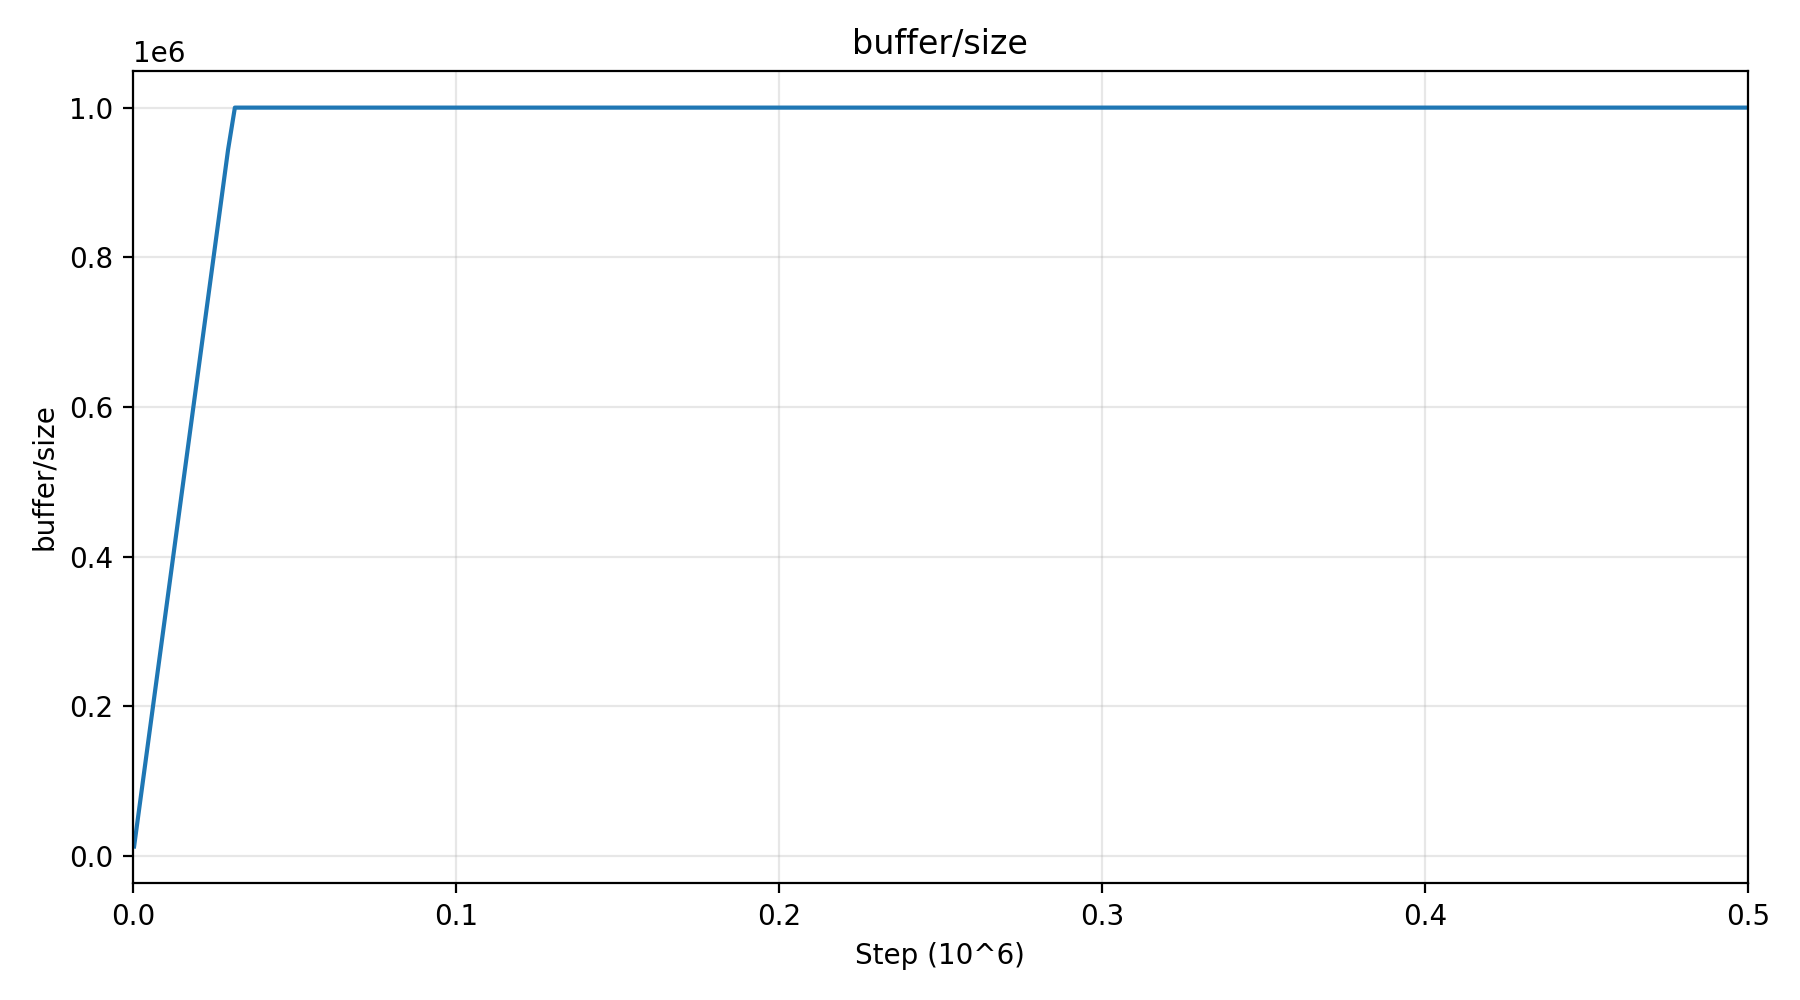
\includegraphics[width=0.5\textwidth]{figures/buffer.png}
  \caption{ASL架构训练时共享数据中枢的经验池占用率分析}
  \label{fig:buffer-analysis}
\end{figure}
由图\ref{fig:buffer-analysis} 可见，ASL 架构的共享数据中枢在训练过程中表现出极高的稳定性与效率：在横轴（Step）的最左侧，紫线几乎是垂直向上飙升的。这表明系统在训练初期就迅速填满了经验池，达到了预设的 100 万条转移数据的容量上限。随后，经验池的占用率曲线趋于平坦，稳定在 100\% 的水平，说明系统成功实现了环形覆盖机制，同时侧面印证了ASL系统的采集数据高效性。

\subsection{SAC算法评估分析}
\begin{figure}[H]
  \centering
  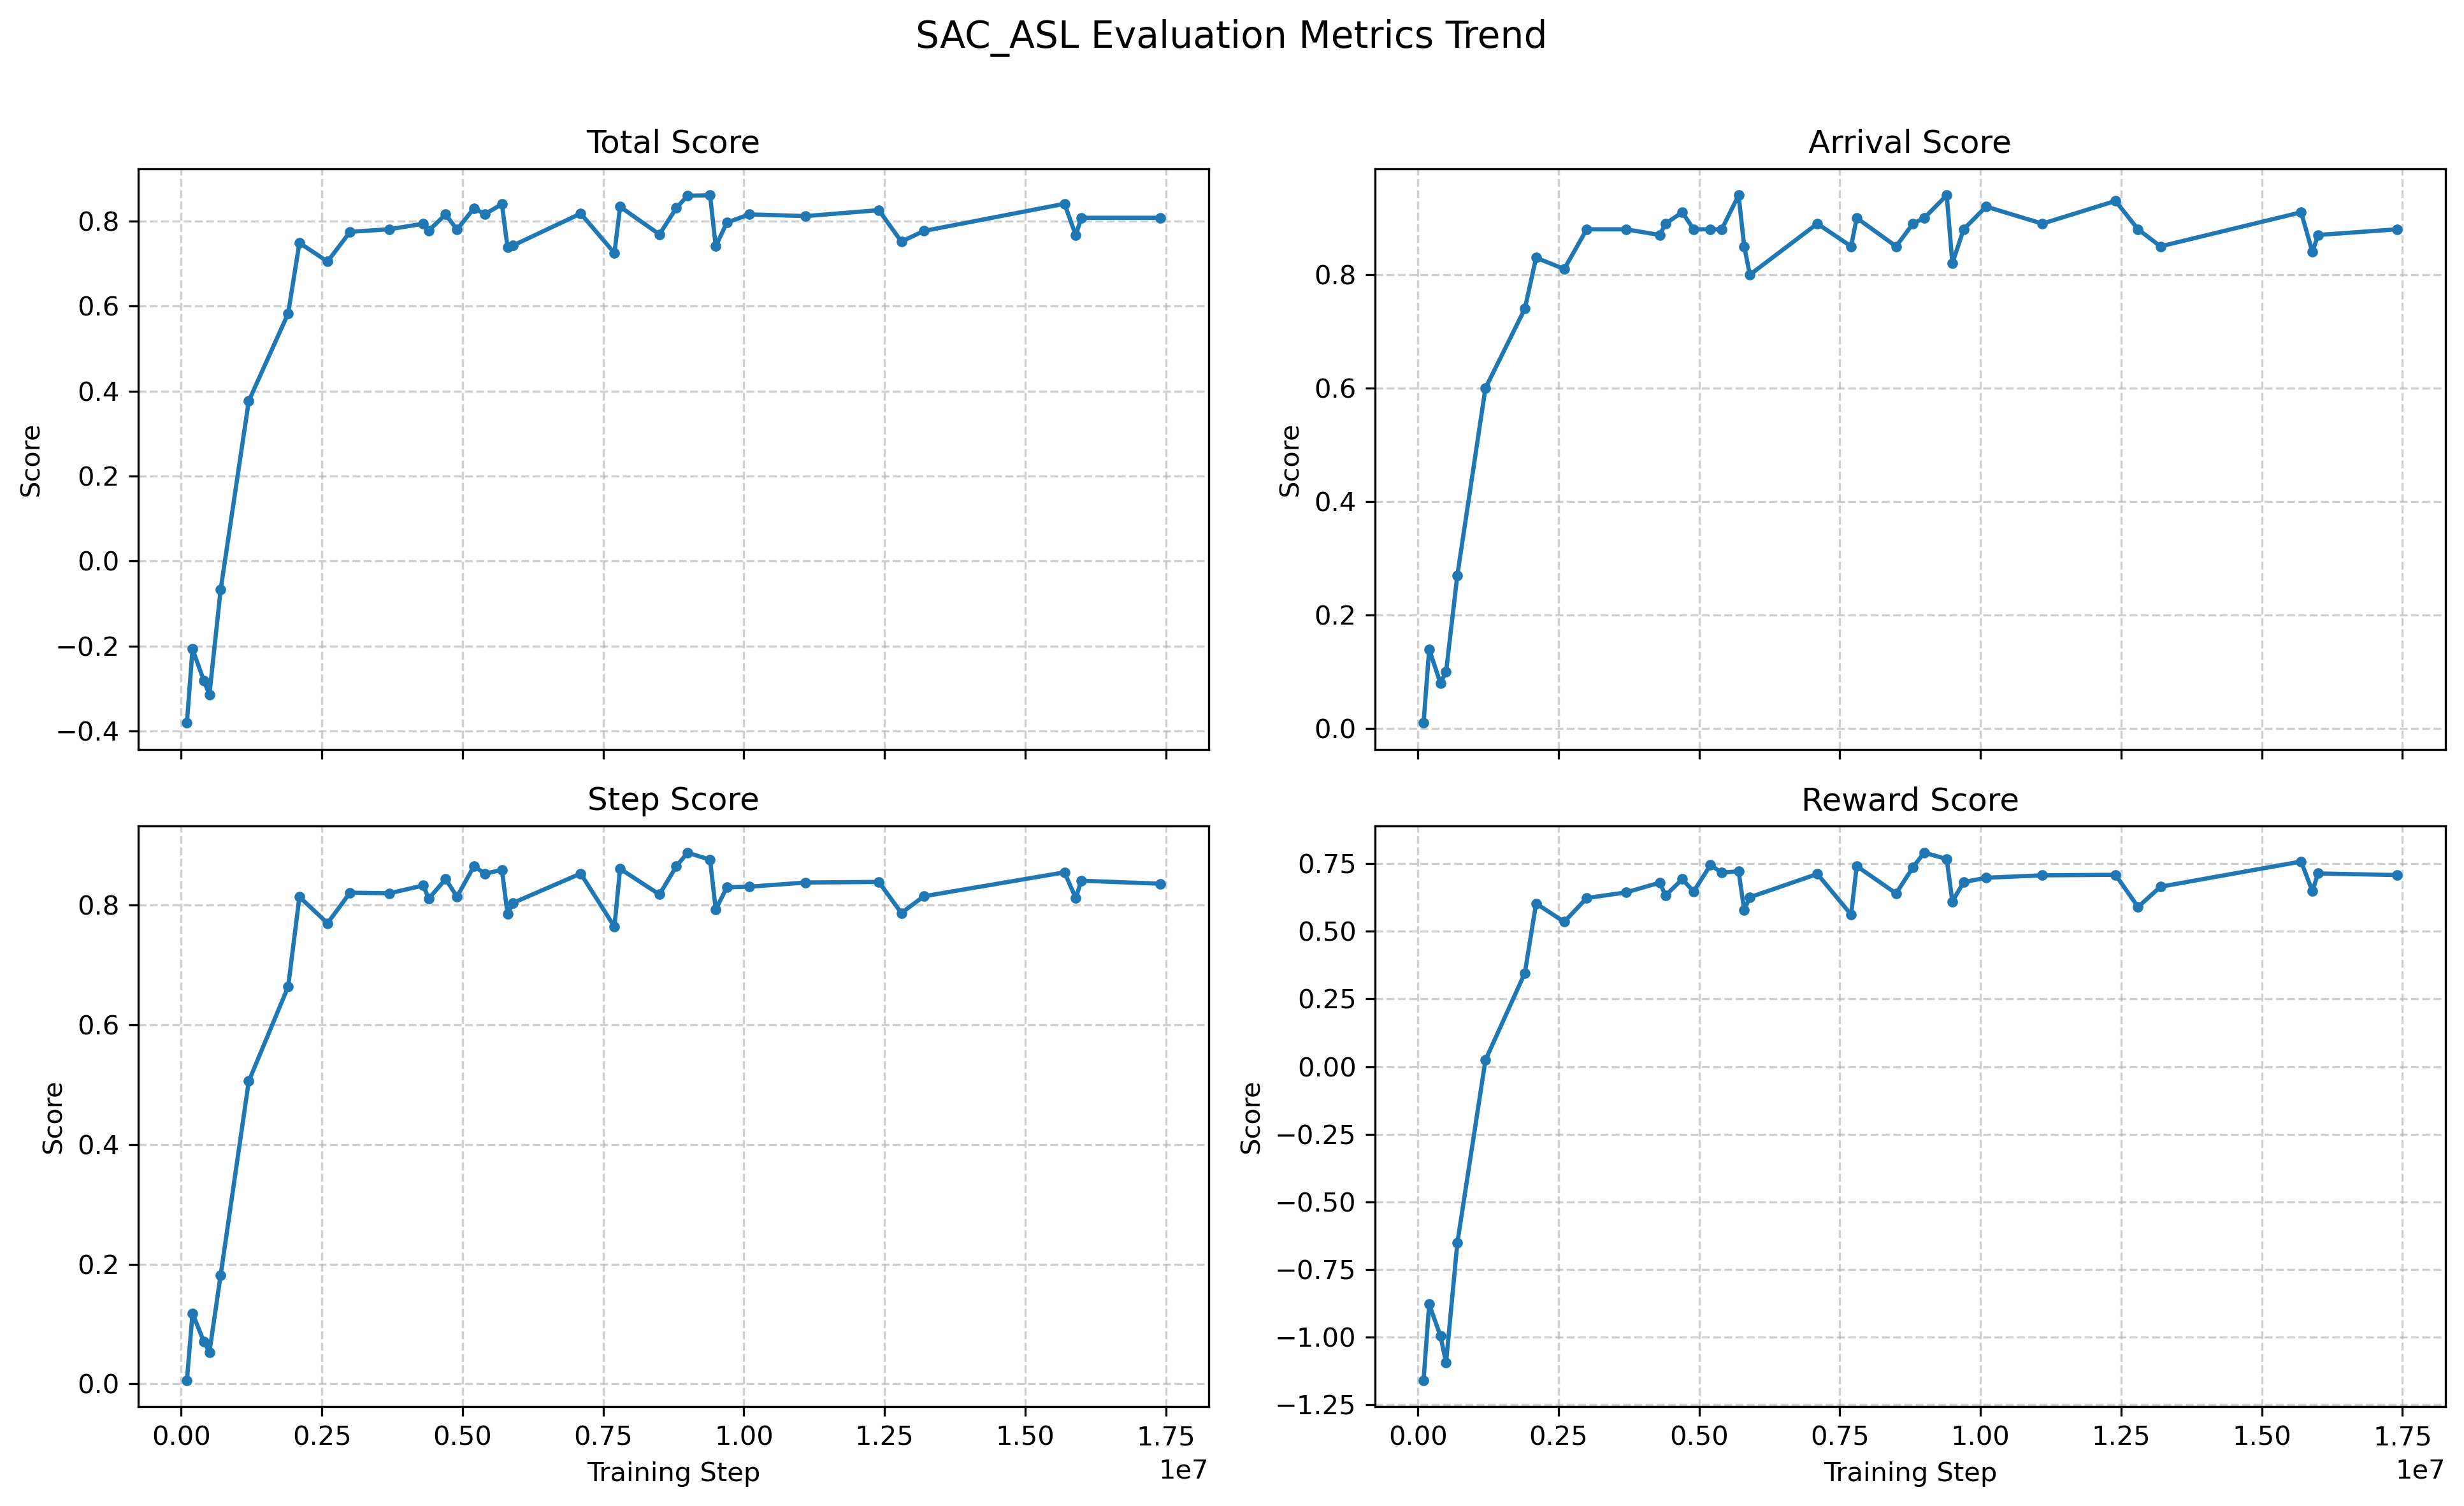
\includegraphics[width=0.7\textwidth]{figures/SAC_ASL_metrics_trend.png}
  \caption{SAC算法到达率、平均每回合步数和平均每回合奖励的训练趋势展示}
  \label{fig:sac-showcase}
\end{figure}

与传统强化学习算法相比，SAC\_ASL 表现出了极其优异的起步学习能力。在训练的极初期（约 $0$ 至 $0.25 \times 10^7$ 步），所有四项指标均呈现出几乎垂直的陡峭上升趋势。这表明该算法能够更高效地利用收集到的样本数据，在极短的探索期内便构建出了高质量的初始策略框架，大幅缩短了模型预热时间。

观察收敛后的曲线（$0.5 \times 10^7$ 步之后），可以发现指标在高位维持整体稳定的同时，伴有偶尔的局部下探（例如在约 $0.6 \times 10^7$ 和 $1.3 \times 10^7$ 步处）。这种现象高度符合 SAC 算法体系的特征：其内建的最大熵强化学习框架促使智能体在利用已知最优策略的同时，始终保持一定程度的随机探索。这种机制虽然会导致分数的短暂波动，但有效防止了模型陷入局部最优解，并在遭遇性能波动后能够迅速自我修复回到高分基线，证明了策略具备极强的鲁棒性。

综合而言，SAC\_ASL 算法在该实验环境中不仅收敛速度极快，且最终能够收敛到一个具备极高成功率和高效执行能力的策略上，充分验证了该算法（或改进机制）在当前复杂任务场景下的有效性与先进性。

\section{TransSAC算法调试}
\subsection{TransSAC算法实现与时序上下文增强}
TransSAC 是本文在 SAC 基础上的进一步增强版本，其核心思想是利用 Transformer 对历史状态序列进行编码，从而弥补标准 SAC 对短期上下文建模不足的问题。对于路径规划任务而言，机器人当前时刻的观测往往无法完整反映动态障碍物的运动趋势，尤其是在障碍物连续移动、环境反馈具有滞后性的情况下，单帧状态输入很容易导致策略出现“看见当前、忽略趋势”的局限。Transformer 的引入正是为了解决这一问题。

在实现上，本文将近期若干步的状态特征拼接为序列输入，通过自注意力机制提取其中的关键时序依赖，再将增强后的上下文特征送入 SAC 的策略网络与价值网络。这样做的直接收益是，模型不仅能判断“此刻是否安全”，还能更早捕捉障碍物的运动方向和目标区域的变化趋势，从而在决策上表现出更强的前瞻性。相比普通 SAC，TransSAC 往往在训练初期就能形成更稳定的动作偏好，路径选择也更少出现反复修正。

从训练表现来看，TransSAC 的优势主要体现在样本效率和早期收敛速度上。虽然其网络结构更复杂、单步计算开销略高，但由于时序特征提取更充分，策略可以更快建立对环境动态的稳定认知，因此在相同训练轮数下通常能获得更高的到达率和更低的平均步数。也正因如此，本文将其作为与 SAC 并列的重点对比对象，用于验证 Transformer 在路径规划强化学习中的增益。

TransSAC 在 SAC 基础上引入 Transformer 编码器，使网络能够对历史状态序列进行时序建模。相比于逐帧处理，这一设计使模型能够捕捉环境动态的长期依赖，对于部分可观测环境（POMDP）下的路径规划任务尤为关键。本节介绍其核心架构与调试要点。

\subsubsection{TransSAC 网络结构}
\begin{figure}[H]
  \centering
  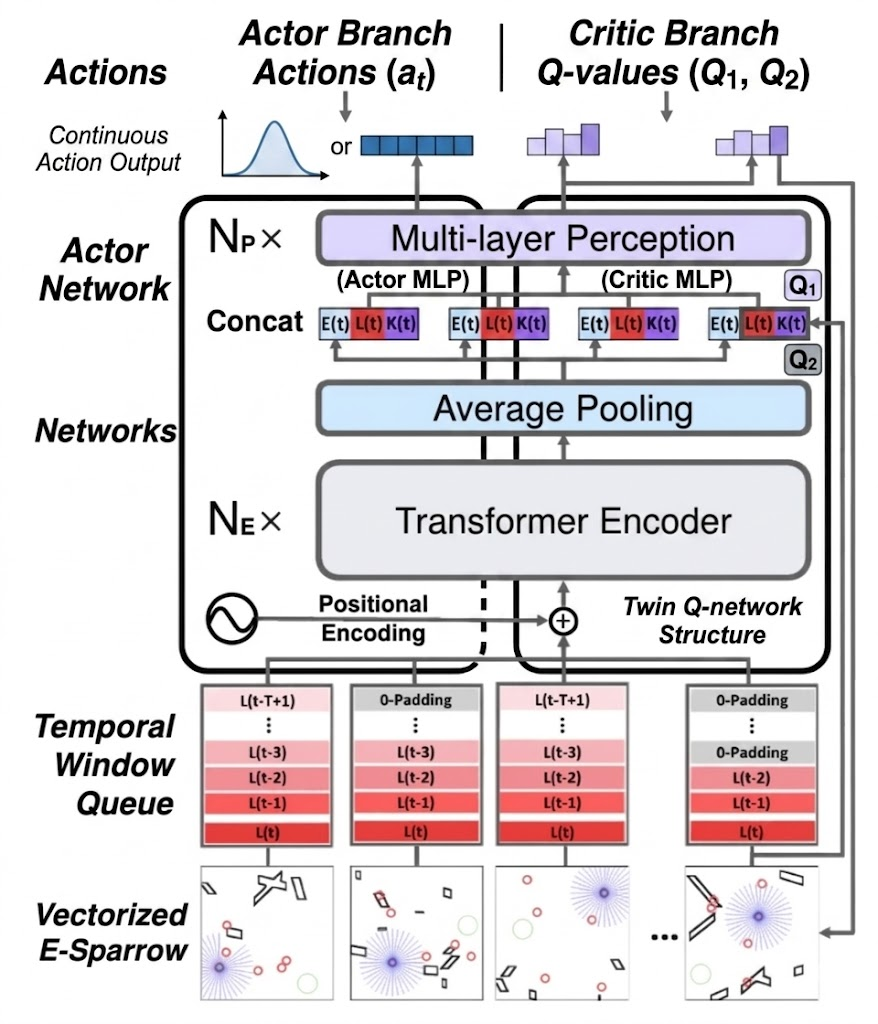
\includegraphics[width=0.5\textwidth]{figures/TransSAC_structure.png}
  \caption{TransSAC 网络结构}
  \label{fig:transSAC-structure}
\end{figure}

如图\ref{fig:transSAC-structure}所示，系统维护一个长度为 $T$ 的时序窗口队列，存储最近 $T$ 个时刻的向量化观测值 $\{L(t-T+1), \dots, L(t)\}$。TransSAC 的状态表示由这一时序窗口组成 $\mathbf{s}_t = \{l_{t-T+1}, \dots, l_t\}$。

特征提取过程定义如下：先通过位置编码（Positional Encoding）为序列添加时间信息，随后经 $N_E$ 层 Transformer 编码块进行自注意力编码，最后通过全局平均池化压缩为固定维度的特征向量：

\begin{equation}
    \mathbf{z}_t = \text{AvgPool}(\text{TransformerEnc}(\mathbf{s}_t + \text{PE}))
\end{equation}

其中，$\text{PE}$ 为位置编码，$\mathbf{z}_t \in \mathbb{R}^{d_{feat}}$ 为增强后的全局特征。

Actor 与 Critic 网络分别以 $\mathbf{z}_t$ 作为输入，输出为：

\begin{align}
    \pi(a_t|s_t) &= \mathcal{N}(\mu_{\theta}(\mathbf{z}_t), \sigma_{\theta}(\mathbf{z}_t)) \\
    Q_{\phi}(\mathbf{s}_t, a_t) &= \text{MLP}_{\phi}(\text{Concat}(\mathbf{z}_t, a_t))
\end{align}

Actor 网络经过 $N_P$ 层 MLP 后输出策略分布参数；Critic 包含两个独立的 Q 网络，以实现 SAC 的双采样机制并缓解 Q 值高估。

\subsubsection{时序特征提取的优势}

与标准 SAC 相比，TransSAC 在以下方面表现出优势：

\begin{enumerate}
    \item 动态环境感知：Transformer 的自注意力机制能够自适应地学习历史状态中的关键时间步，使模型对动态障碍物的运动轨迹形成更准确的预判。
    \item 降低路径抖动：时序上下文能够稳定策略的决策过程，避免单帧观测导致的前后不一致的动作选择。
    \item 提升样本效率：通过编码足够的历史信息，网络能够更快地学到有效策略，整体收敛速度超过逐帧处理的方案。
\end{enumerate}

\subsection{Transformer训练调试与超参数配置}
\begin{figure}[H]
  \centering
  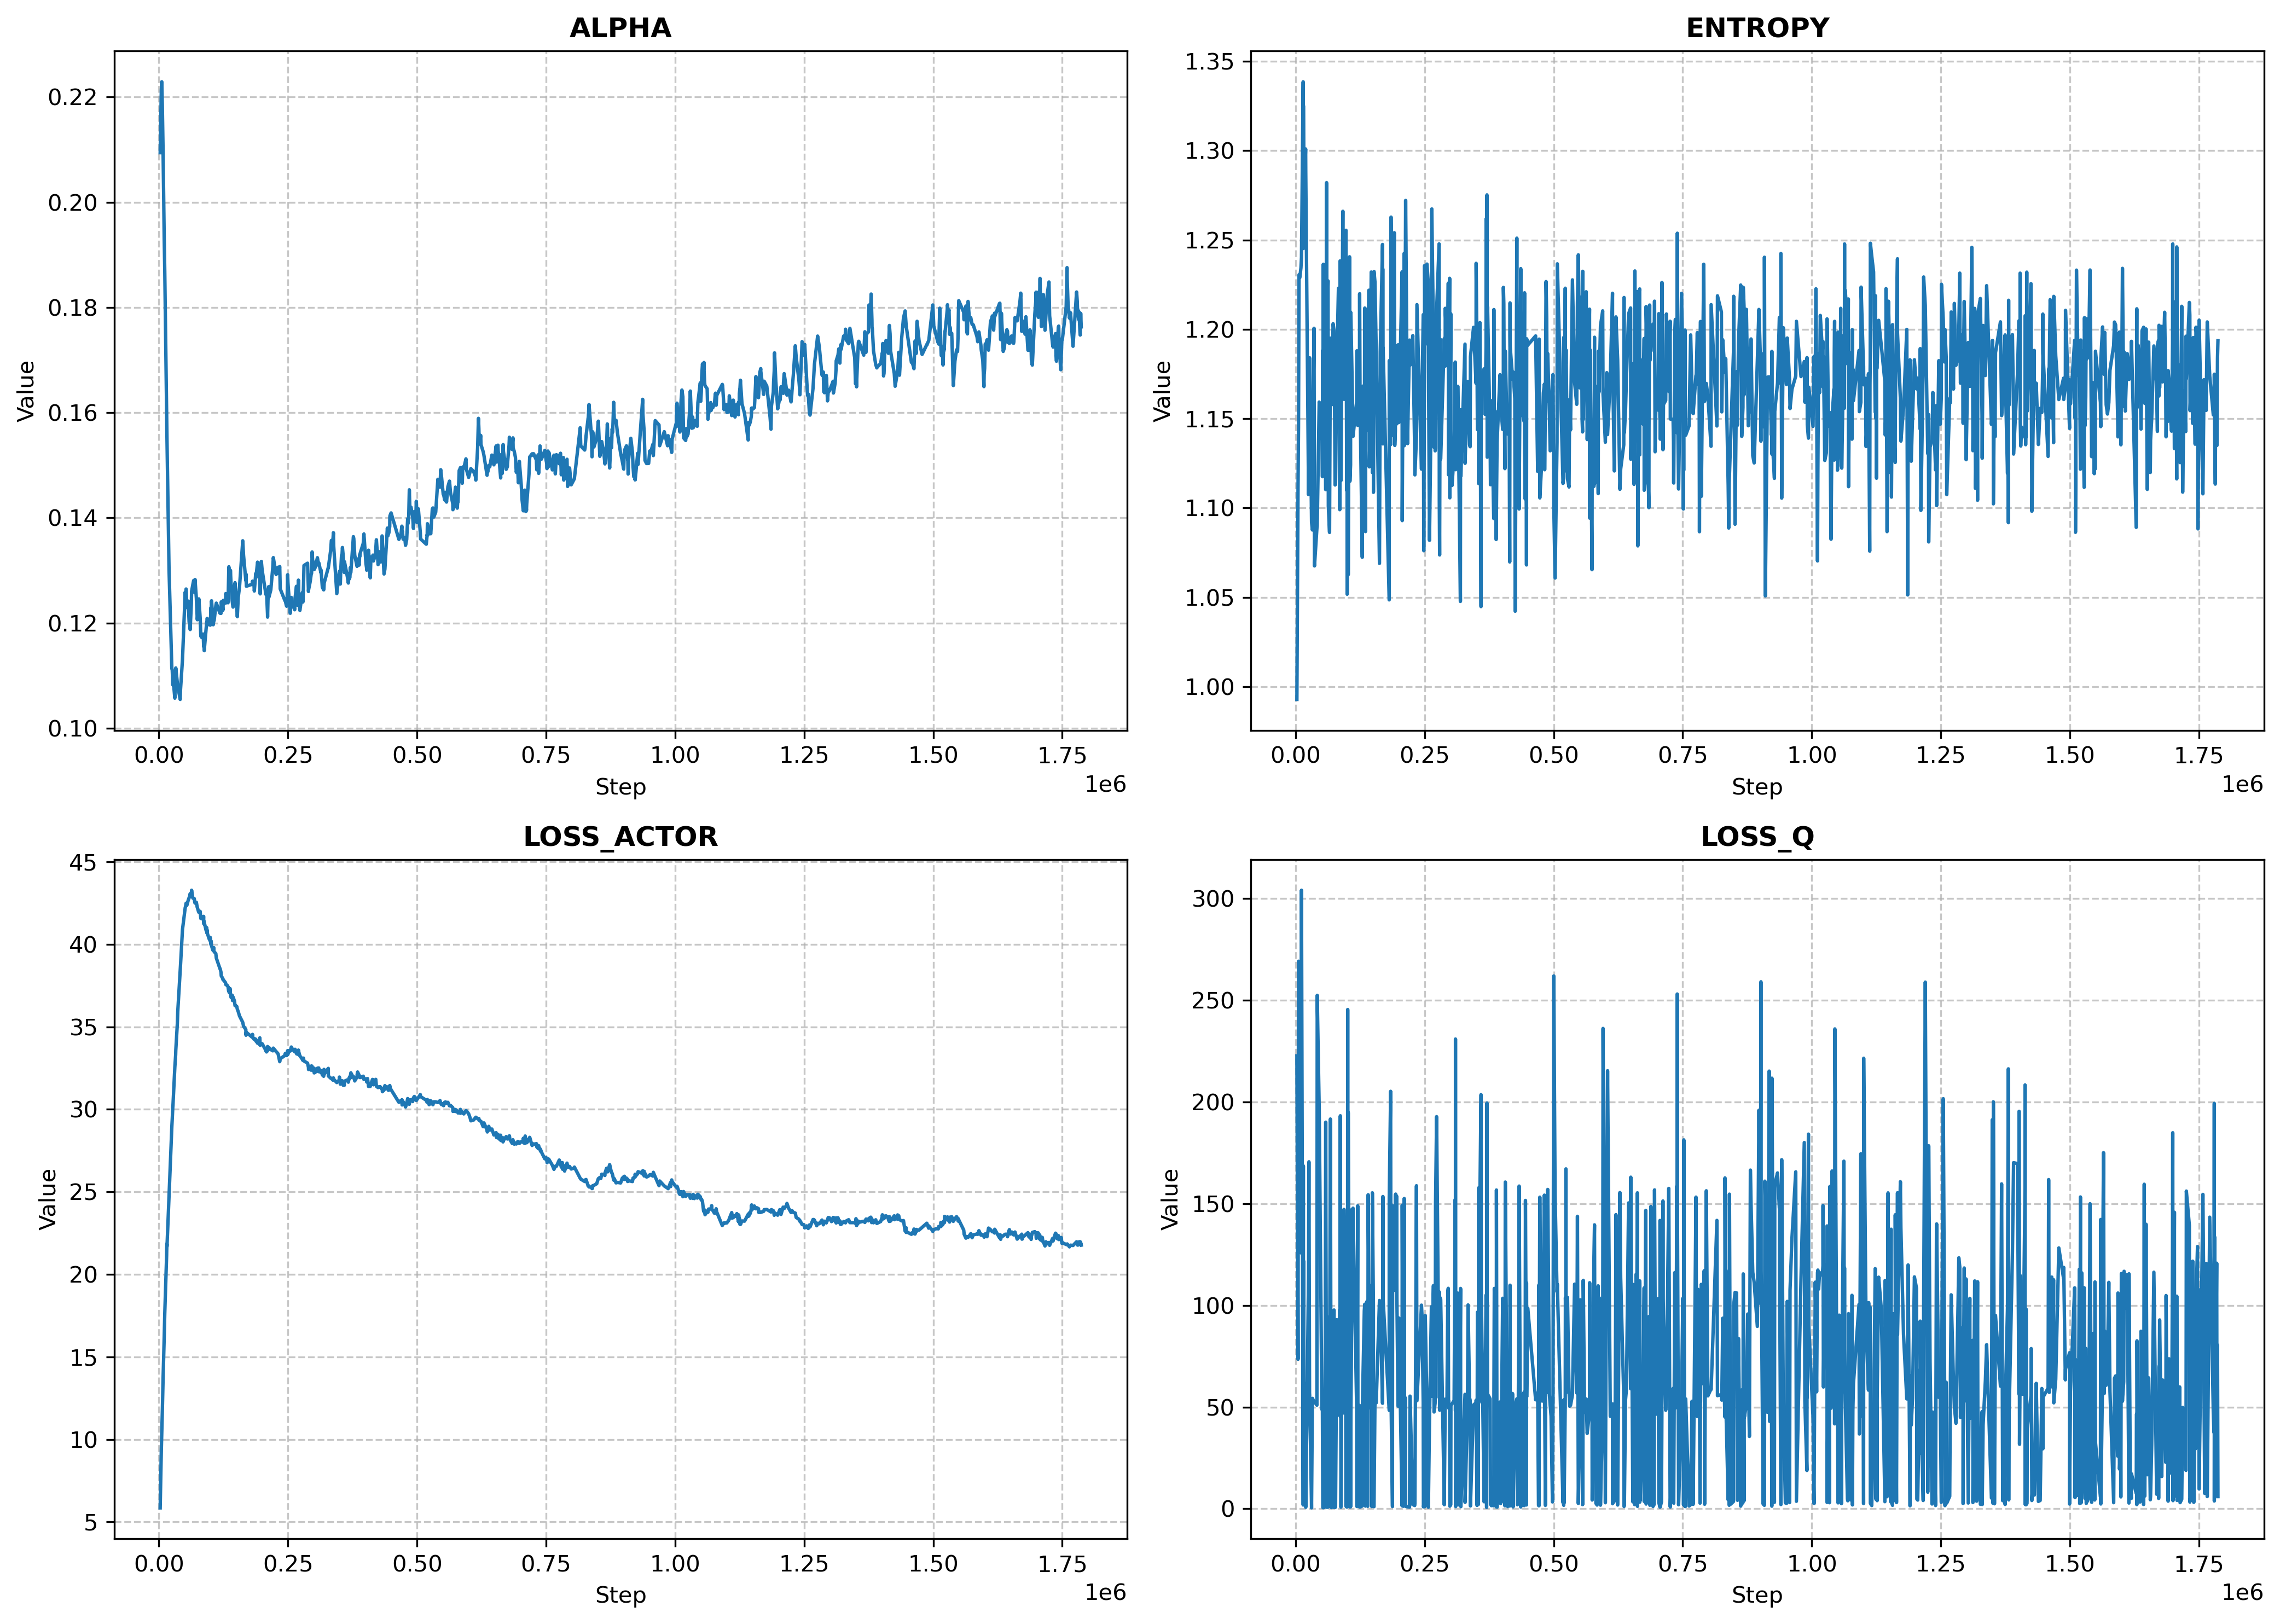
\includegraphics[width=0.7\textwidth]{figures/bad_transSAC/bad_transSAC_ASL_train_combined.png}
  \caption{TransSAC 训练中策略网络崩塌训练记录}
  \label{fig:transSAC-train-bad}
\end{figure}
\begin{figure}[H]
  \centering
  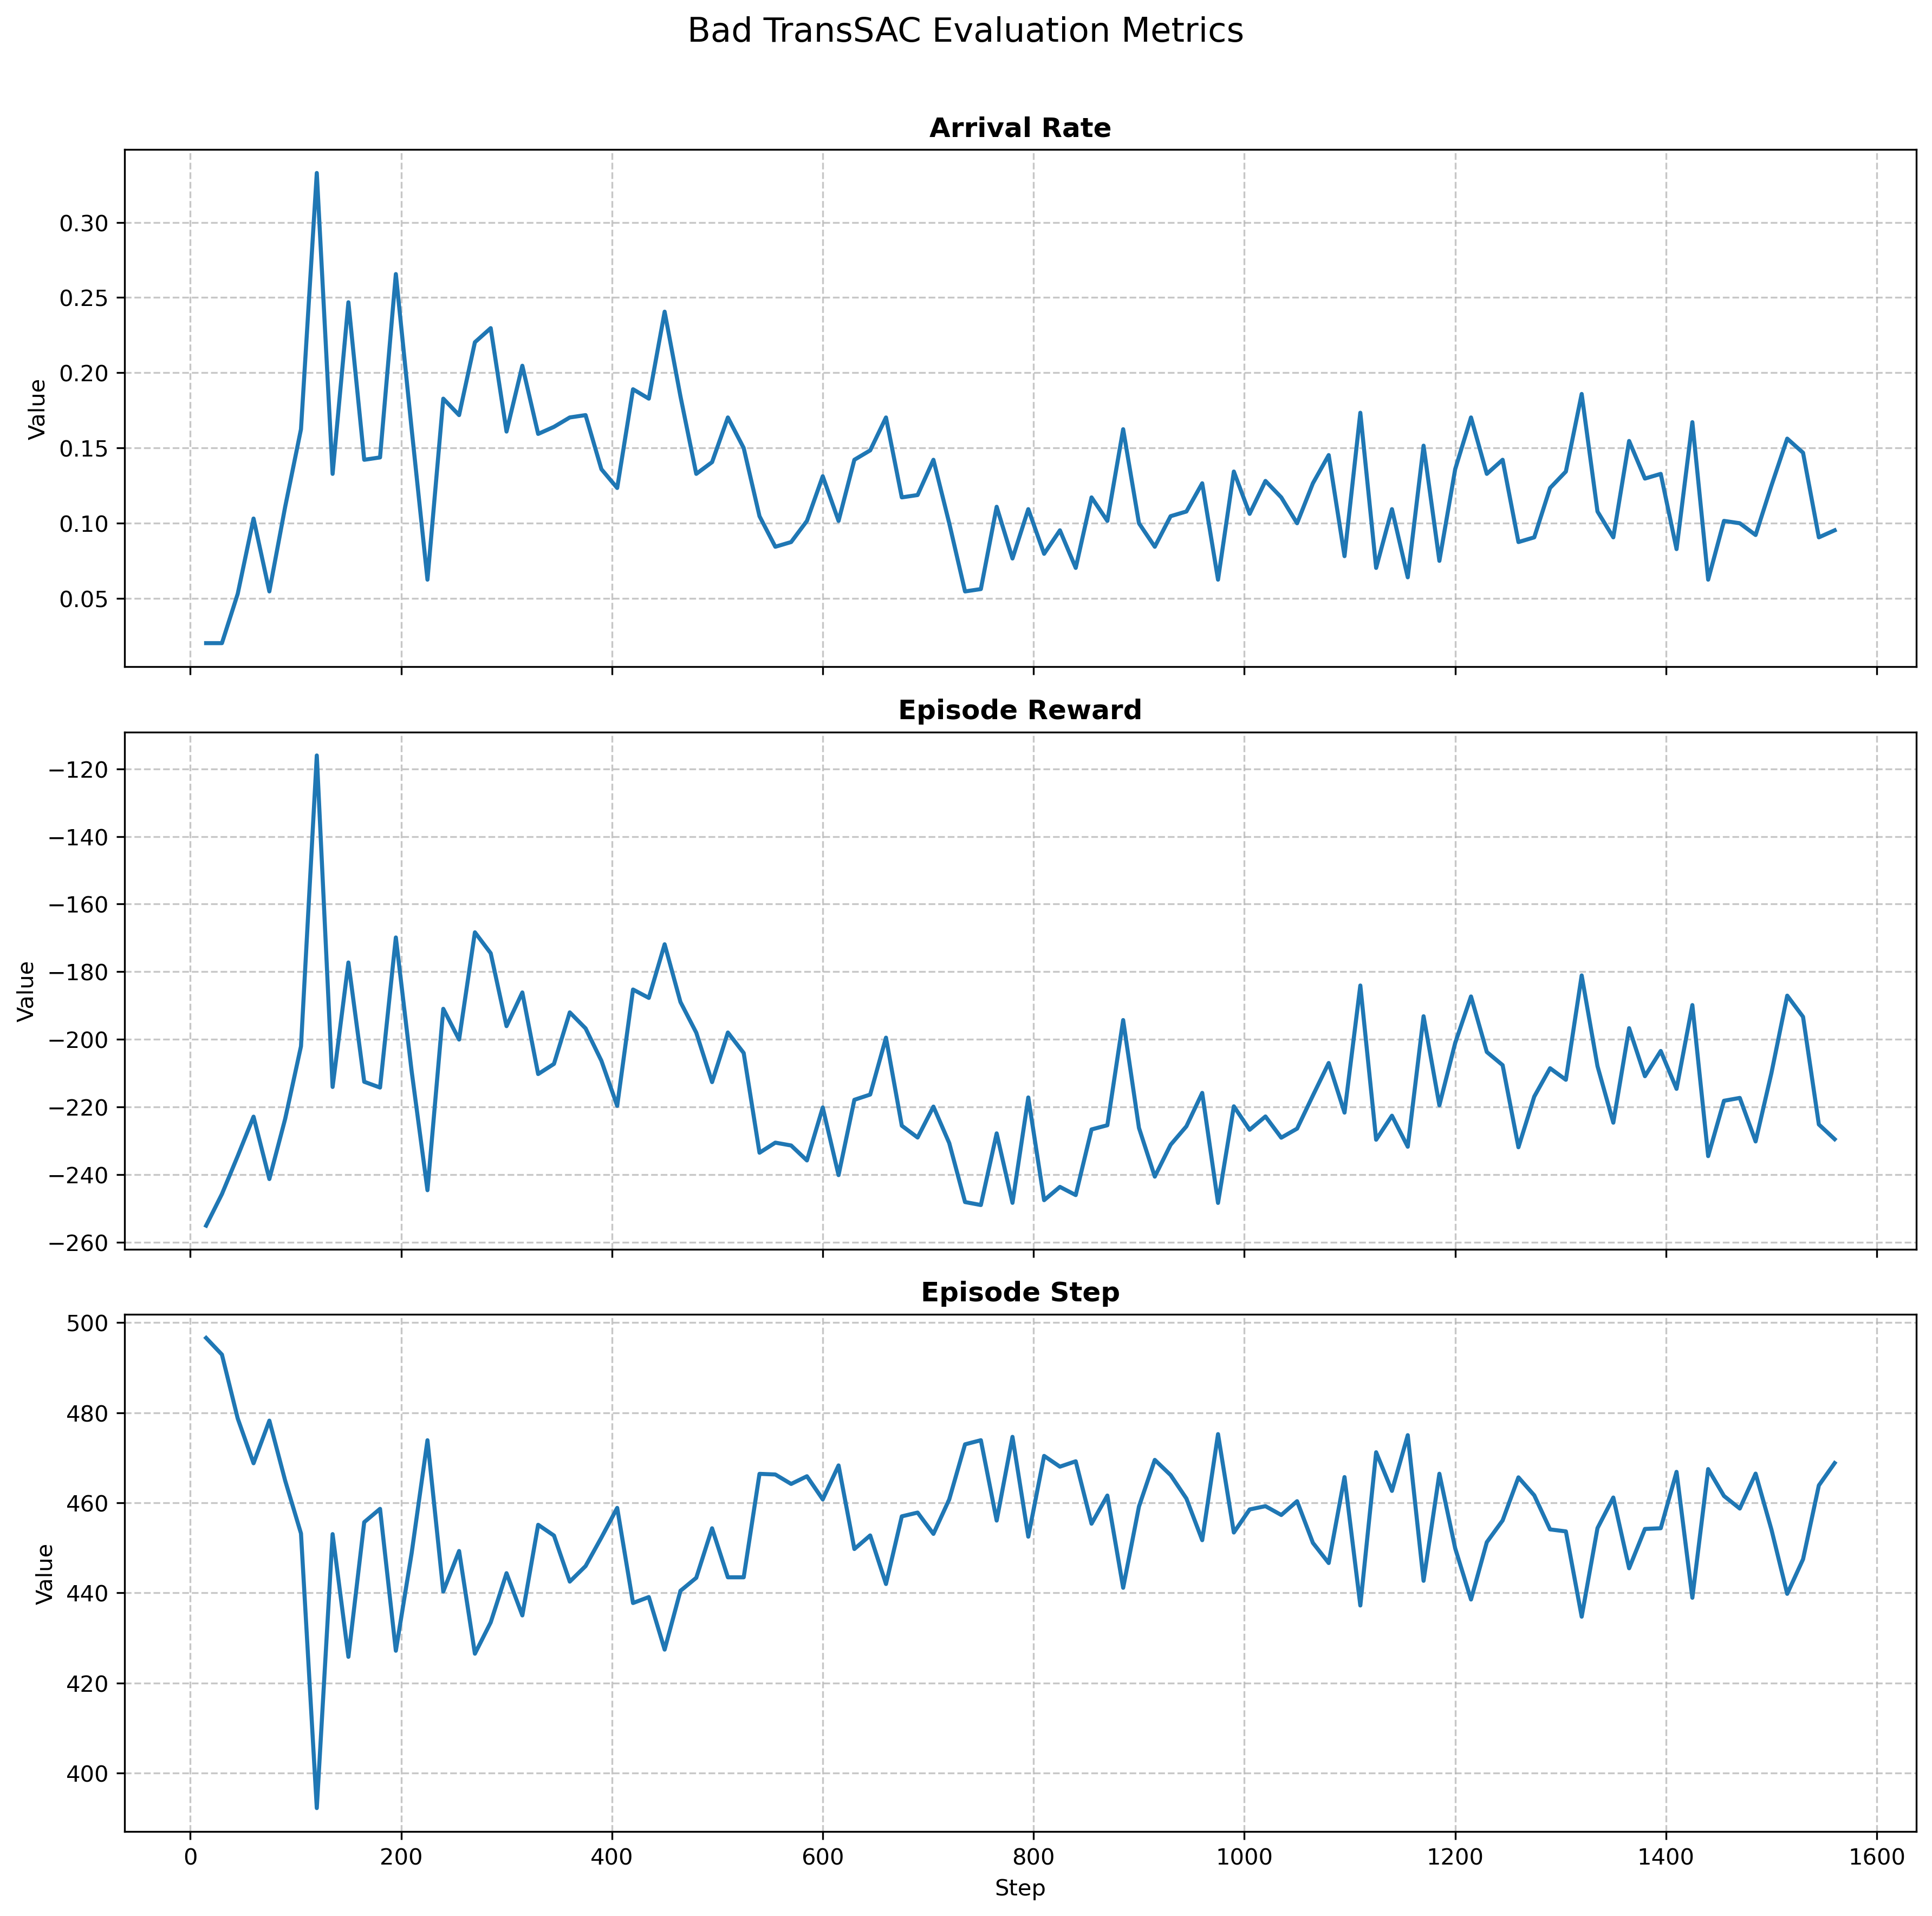
\includegraphics[width=0.7\textwidth]{figures/bad_transSAC/bad_transSAC_eval_combined.png}
  \caption{TransSAC 训练中策略网络崩塌评估结果}
  \label{fig:transSAC-eval-bad}
\end{figure}

如图 \ref{fig:transSAC-train-bad} 与图 \ref{fig:transSAC-eval-bad} 所示，TransSAC 模型在训练初期面临显著的策略网络崩塌（Policy Collapse）挑战。训练过程中 Actor 的奖励曲线出现剧烈震荡，并在数千步内急剧下降至接近零的水平，表明策略网络未能有效学习到具有指导意义的动作分布，导致智能体行为退化为无效的随机探索。评估结果同样显示，智能体到达目标点的成功率在训练初期徘徊在 0\% 至 20\% 的低位，且累计奖励极低，进一步印证了策略崩塌对模型导航性能的严重破坏。

结合 Transformer 架构对序列异常值的敏感度与离策略（Off-policy）强化学习的训练动态，可将策略崩塌的潜在诱因归纳为以下三个维度：

\begin{enumerate}
    \item Q网络损失爆炸与剧烈震荡：Critic 网络的损失（Loss/Q）高达 300 以上且震荡剧烈，说明 Q 网络无法有效拟合时序差分目标（TD Target）。这通常源于环境奖励尺度过大、学习率配置过高或梯度截断机制的缺失。
    \item Actor网络损失持续攀升： 在 SAC 算法框架中，Actor 的优化目标为最大化 $Q$ 值与策略熵之和（即 $\alpha \log(\pi) - Q$）。由于 Q 值的发散与崩溃，Actor 的损失随之异常走高，彻底失去梯度的指导意义。
    \item 负向奖励陷阱：平均训练奖励（Train/RewardMean）恒为负值且完成率（Train/DoneRate）趋近于零，表明智能体持续触发惩罚机制（如碰撞障碍物），深陷局部次优策略而未能采集到正向奖励样本。
\end{enumerate}

由于本研究模型融合了 Transformer 结构，其自注意力（Self-Attention）机制中的连乘操作对序列特征的异常波动极度敏感。若在强化学习中未对 Critic 网络施加严格的梯度裁剪（Gradient Clipping），或者批次大小（Batch Size）不足以平滑序列特征分布，反向传播时的 TD 误差极易引发梯度爆炸。

鉴于上述分析，本研究首先对 Transformer 网络架构进行轻量化降维处理，采用单层编码器（$L=1$）与 4 组注意力头（$H=4$）的基础配置以降低初期拟合难度；同时，对 Critic 网络独立配置较小的学习率（$\mathrm{lr}_{\mathrm{critic}}=5 \times 10^{-5}$），以平抑训练初期的极端梯度波动。密切监控 Critic 的损失曲线与 TD 误差分布，确保其在合理范围内波动。

为进一步确保模型在复杂连续状态空间中实现稳定收敛，本研究在算法的工程实现层面引入了一系列训练稳定性保障机制，具体阐述如下：

\begin{enumerate}
    \item 基于渐进式环境复杂度的课程学习：针对智能体在冷启动阶段面临的极高探索壁垒，引入了“小步前进”（Baby Step）的渐进式课程学习机制。在总训练步数的前 15\% 阶段，系统动态调整环境配置，使障碍物密度与动态难度呈阶梯式递增。该策略有效规避了智能体在初期因频繁触发高额惩罚而导致的策略崩溃，稳妥地引导模型度过脆弱的随机探索期。
    
    \item 自适应梯度裁剪机制： 为抑制深层网络及 Transformer 自注意力机制中频发的梯度爆炸问题，在反向传播更新参数前引入了全局梯度范数裁剪。针对不同模块的参数敏感度，设定了差异化的截断阈值：对高敏感的 TransSAC 主干网络采取严苛的裁剪标准（$\max\_norm=0.5$）；而对 ASL 分布式架构中的Learner模块采用相对温和的阈值（$\max\_norm=10$）。该机制从物理层面约束了单次参数更新的最大步幅，保障了优化轨迹的平滑可控。
    
    \item 正交权重初始化：针对深层神经网络易出现的梯度消失或特征方差偏移现象，采用正交矩阵对线性层权重进行初始化，并设定适配 ReLU 激活函数族的缩放因子 $\text{Gain} = \sqrt{2} \approx 1.414$。正交矩阵的保范数特性确保了跨层信息传递时梯度能量的一致性，从先验层面极大增强了深层网络的数值鲁棒性。
    
    \item 数值稳定性保护：在计算策略熵与对数概率时，由于网络易输出趋近于 0 的离散动作概率值，直接求对数会引发 $\log(0) \to -\infty$ 的计算溢出灾难。为此，系统在所有对数求解操作中引入极小数值扰动常数，严格执行 $\log(\pi(a|s) + 10^{-8})$ 的边界约束，以极低的精度代价阻断了由异常值引发的参数崩溃。
    
    \item 安全目标熵修正：在最大熵强化学习框架中，温度系数 $\alpha$ 动态调节着探索与利用的权衡。区别于标准算法将目标熵设定为最大理论熵 0.98 倍的默认配置，本研究经实验观察发现，该比例在复杂的环境分布下会导致 $\alpha$ 值发生不可逆的指数级膨胀，迫使策略退化为纯随机游走。因此，本研究将目标熵的修正比例保守调整为 0.6，在保障必要动作探索空间的同时，有效锁定了 $\alpha$ 参数的收敛上限。
\end{enumerate}

按上述流程逐项排查并调整，最终训练收敛。

\subsection{TransSAC算法评估分析}

评估结果如下：

\begin{figure}[H]
  \centering
  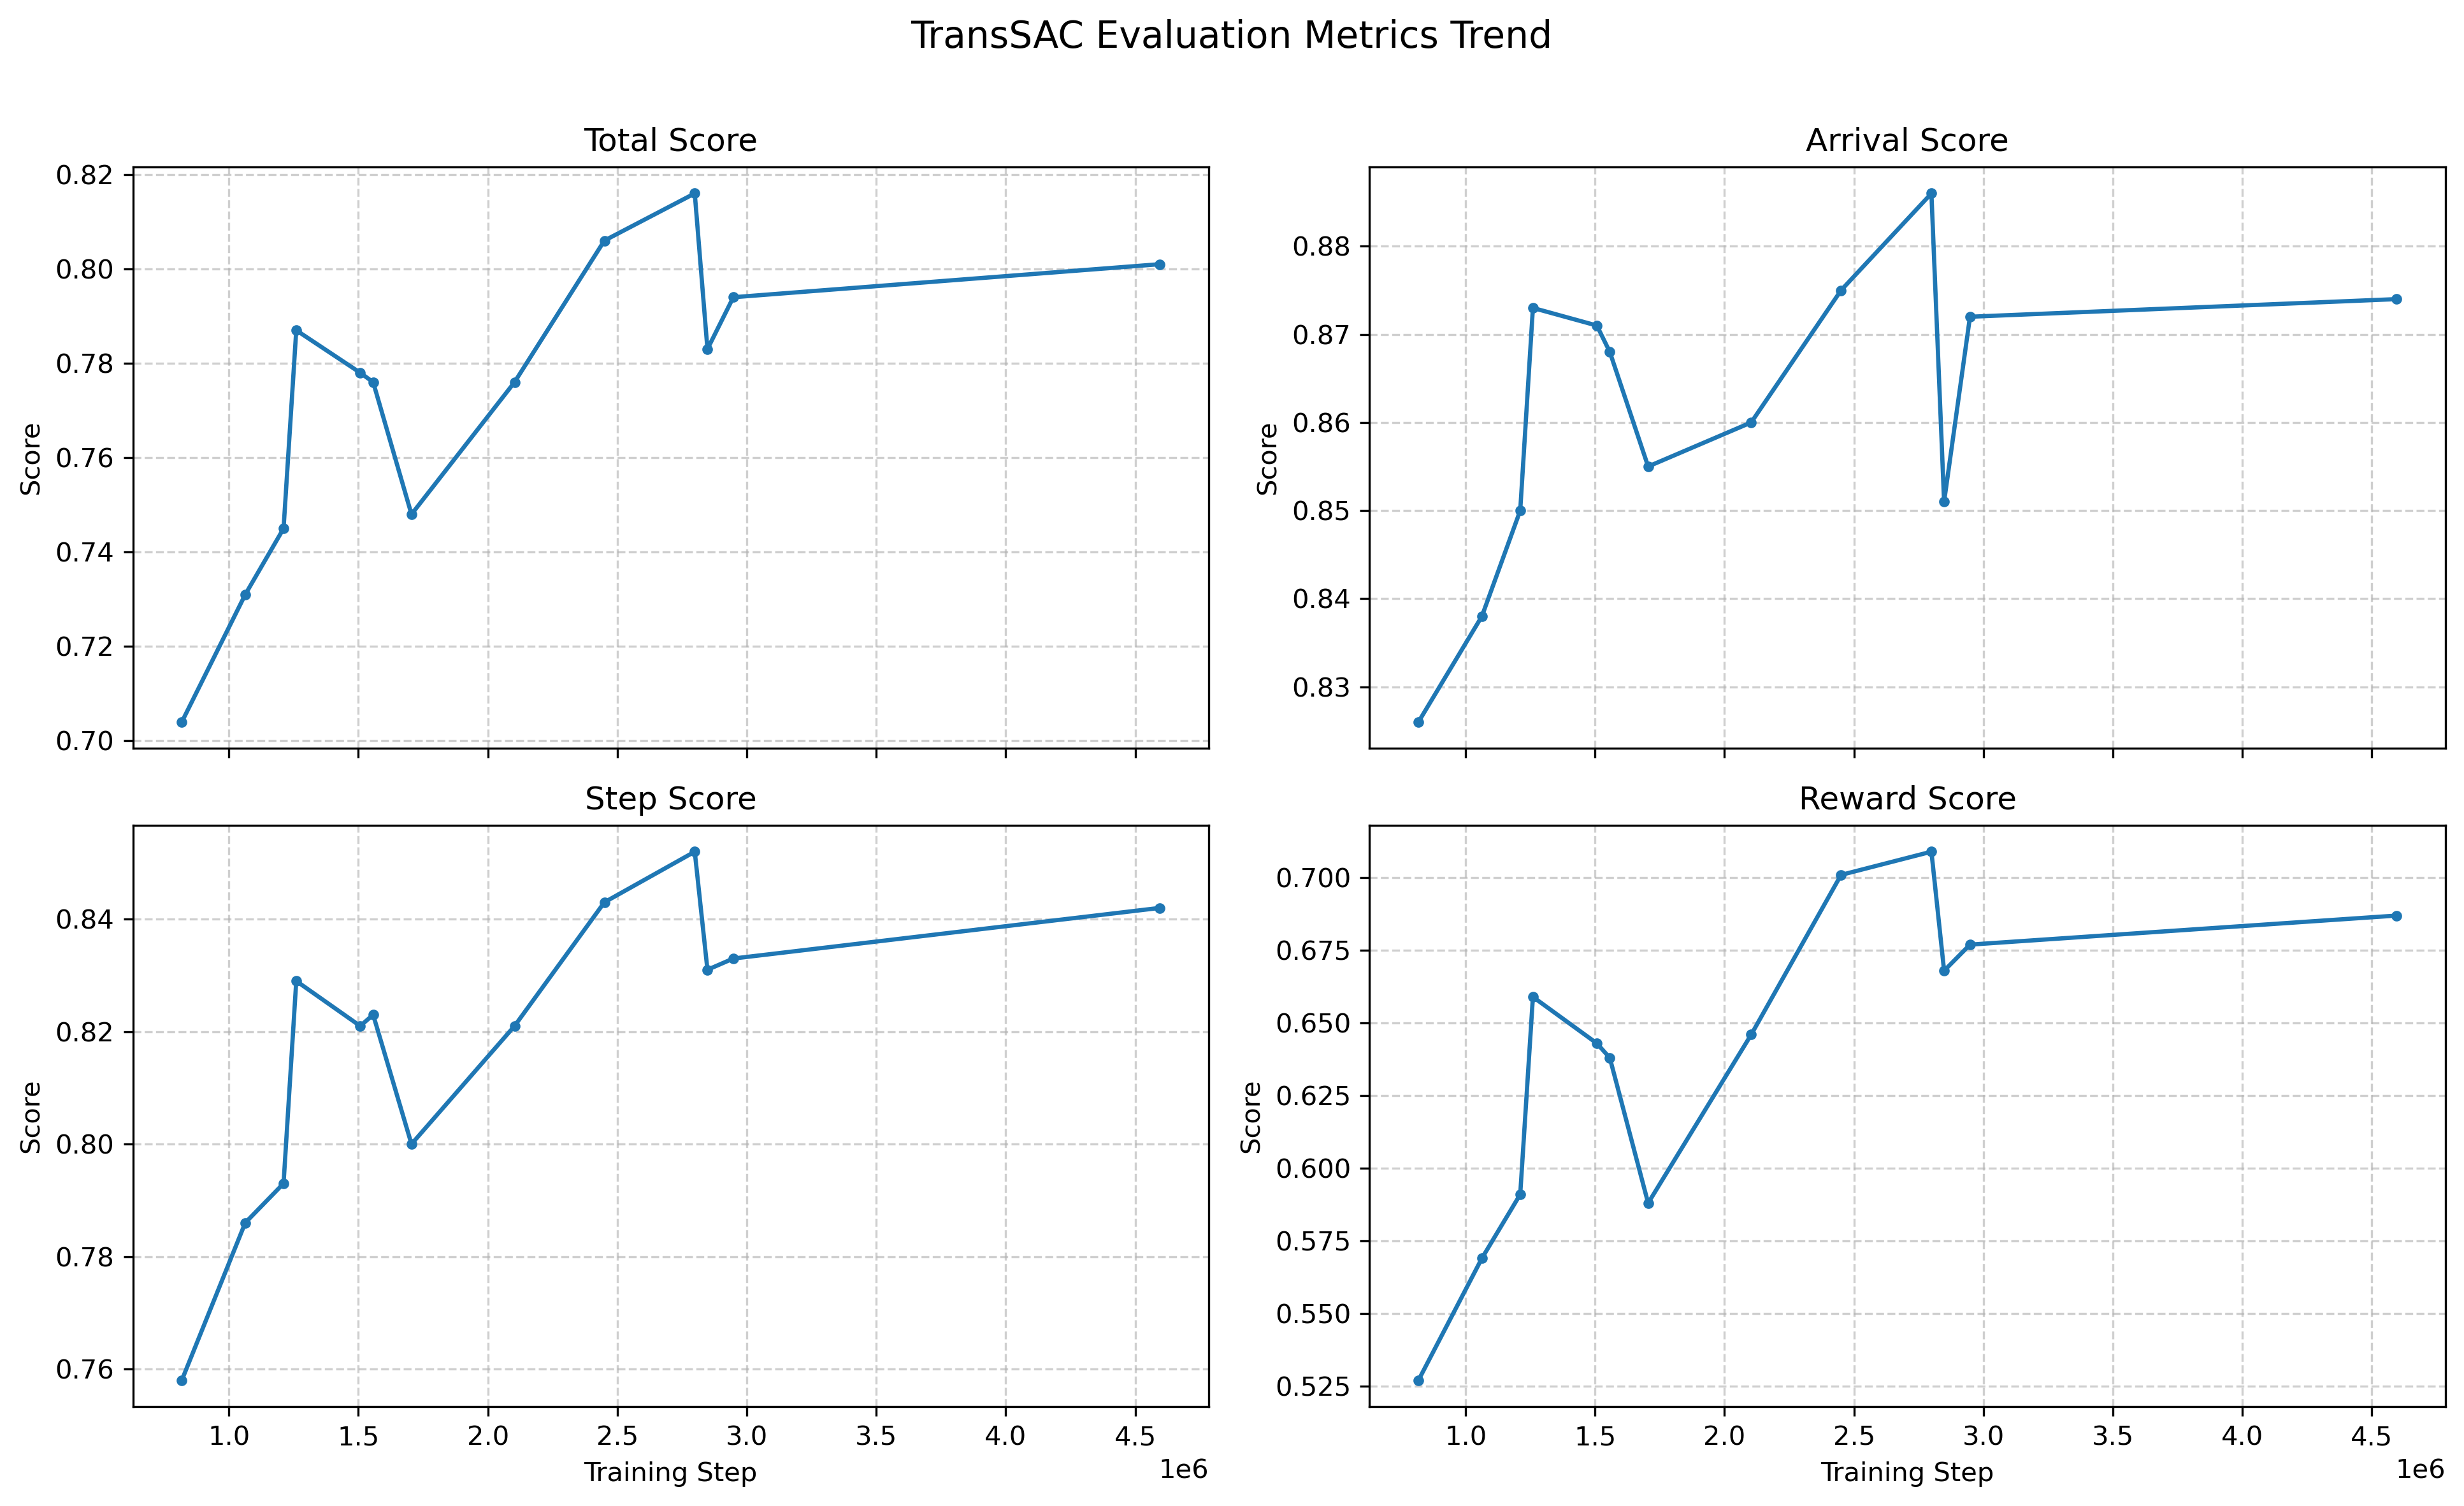
\includegraphics[width=0.7\textwidth]{figures/TransSAC_metrics_trend.png}
  \caption{TransSAC算法到达率、平均每回合步数和平均每回合奖励的训练趋势展示}
  \label{fig:transsac-showcase}
\end{figure}

从整体趋势来看，尽管训练过程伴随着剧烈的波动，但各项指标（总分、到达率、步数得分、奖励得分）均保持了震荡上升的总体态势。在训练接近尾声时，到达率（Arrival Score）回升并稳定在 0.87 左右，总分（Total Score）也逼近 0.80。这表明 TransSAC 算法具备处理复杂导航或控制任务的能力，并最终能够收敛到具有较高成功率的有效策略上。

与传统无模型强化学习算法平滑的收敛曲线不同，TransSAC 在约 $1.5 \times 10^6$ 步与 $2.8 \times 10^6$ 步附近出现了显著的“断崖式”性能下降与随后的快速反弹。这种现象主要源于算法中引入的 Transformer 注意力机制。在探索过程中，由于状态特征序列的多样性，注意力权重的分布容易发生剧烈重构；当智能体探索到未知的状态空间或转移概率发生突变时，价值网络的估计会出现短暂的过拟合或偏差，导致策略评估失准。然而，依赖于 SAC 算法底层的最大熵机制与软更新策略，模型能够在经历挫折后迅速自我纠正，重新找回最优策略梯度，展现出极强的快速恢复能力。

观察“步数得分（Step Score）”与“奖励得分（Reward Score）”的同步下挫与回升，可以发现两者呈现出高度的正相关性。这说明在 Transformer 架构提取高维时空特征时，智能体对路径长度步数和奖励的平衡十分敏感。由于模型容量的增加，网络在拟合复杂状态表征时需要更多的数据样本进行微调，这也是导致训练中期评估指标不稳定的重要原因。

综合来看，TransSAC 牺牲了早期训练的绝对平稳性，换取了对复杂序列特征更强的提取与表征能力。其最终表现出的高到达率证明了该架构在处理需要长期记忆或复杂空间感知任务时的巨大潜力。

相比单纯 SAC，TransSAC 的训练初期即表现出更稳定的到达率（约 50\%），说明时序建模确实带来了决策质量的提升。在后续验证对比中，这一架构的优势将被进一步量化。

\begin{figure}[H]
  \centering
  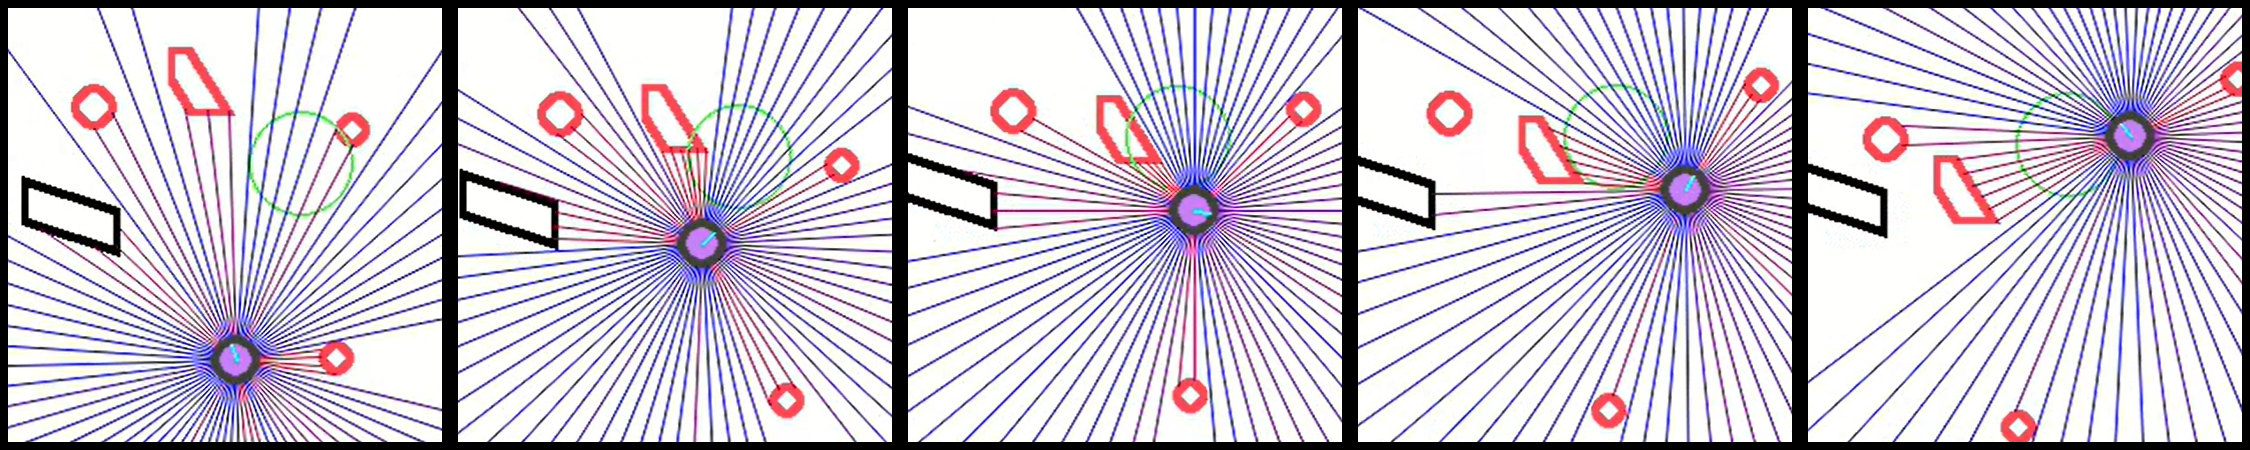
\includegraphics[width=0.7\textwidth]{figures/experiment1_stitched.png}
  \caption{TransSAC 训练中智能体学到的高级避障技能展示（序列1）}
  \label{fig:action_1}
\end{figure}

\begin{figure}[H]
  \centering
  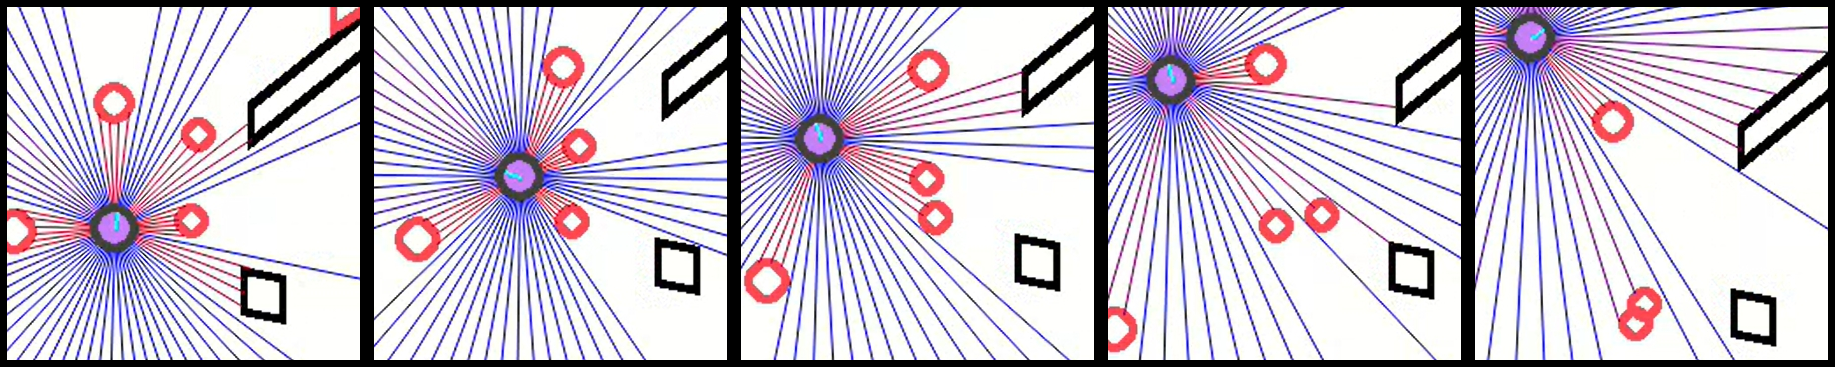
\includegraphics[width=0.7\textwidth]{figures/experiment2_stitched.png}
  \caption{TransSAC 训练中智能体学到的高级避障技能展示（序列2）}
  \label{fig:action_2}
\end{figure}

\begin{figure}[H]
  \centering
  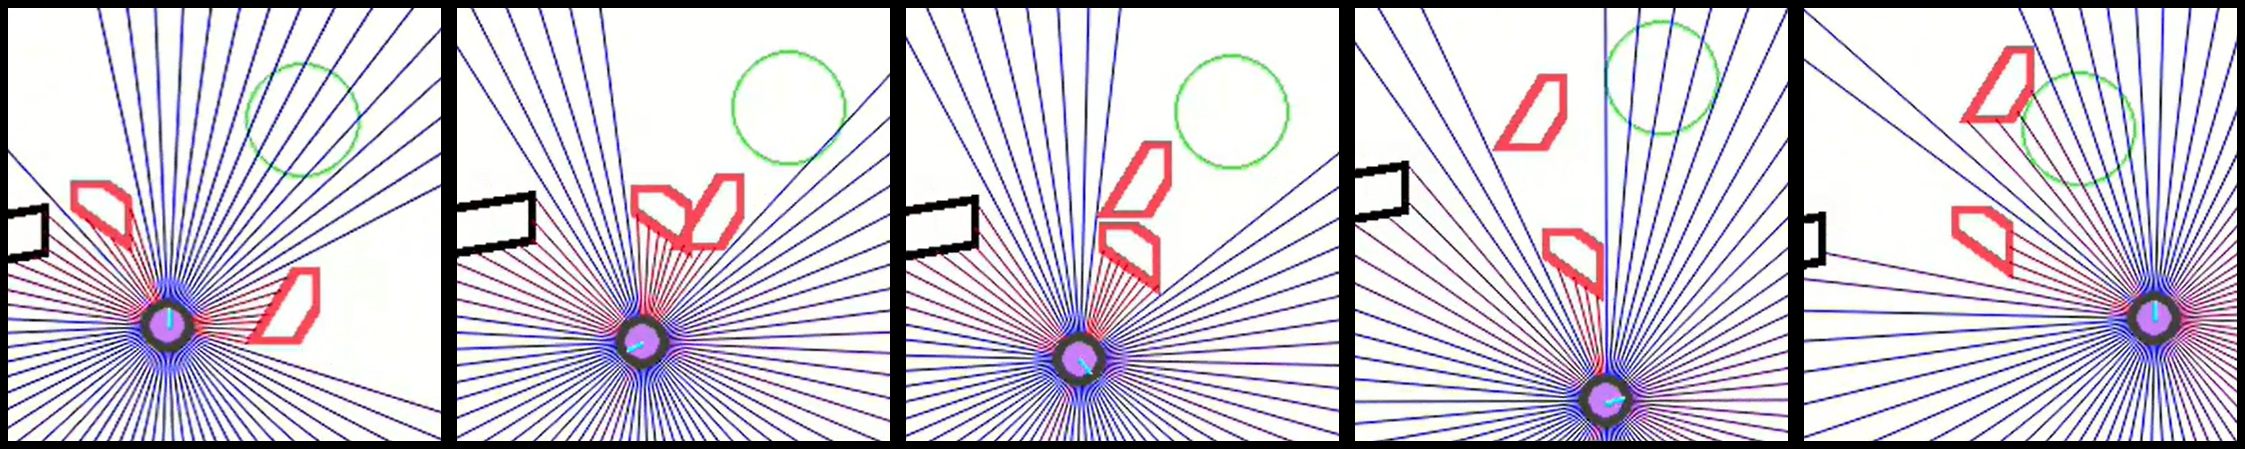
\includegraphics[width=0.7\textwidth]{figures/experiment3_stitched.png}
  \caption{TransSAC 训练中智能体学到的高级避障技能展示（序列3）}
  \label{fig:action_3}
\end{figure}

从上述实验序列可以看出，经过充分训练的 TransSAC 智能体学会了对动态障碍物的主动闪避、等待等在复杂环境中的路径优化的高级导航技能。
\section{路径规划算法对比}

为了全面评估所提出的算法在复杂导航场景下的有效性与优越性，本节开展了详细的比较研究。评估过程主要分为两个维度：首先，将经典的局部路径规划器（DWA）与基于深度强化学习的算法进行基准对比；其次，在强化学习框架内部，对主流的 DQN、SAC\_ASL 算法与本研究提出的 TransSAC 算法进行横向性能剖析。评估的核心指标包括模型训练过程中的到达率（Arrival Rate）、累积奖励（Cumulative Reward）以及任务步数/路径长度（Episode Steps）。

对于DWA经典算法，测试结果如下：
\begin{table}[H]
    \centering
    \caption{DWA经典算法测试结果}
    \label{tab:dwa_eval_result}
    \begin{tabular}{lcccc}
        \toprule
        \textbf{Index} & \textbf{Total Score} & \textbf{Arrival Score} & \textbf{Step Score} & \textbf{Reward Score} \\
        \midrule
        DWA & 0.304 & 0.53 & 0.442 & -0.06 \\
        \bottomrule
    \end{tabular}
\end{table}

对于强化学习算法，不同训练轮数的模型表现如下：

\begin{figure}[H]
  \centering
  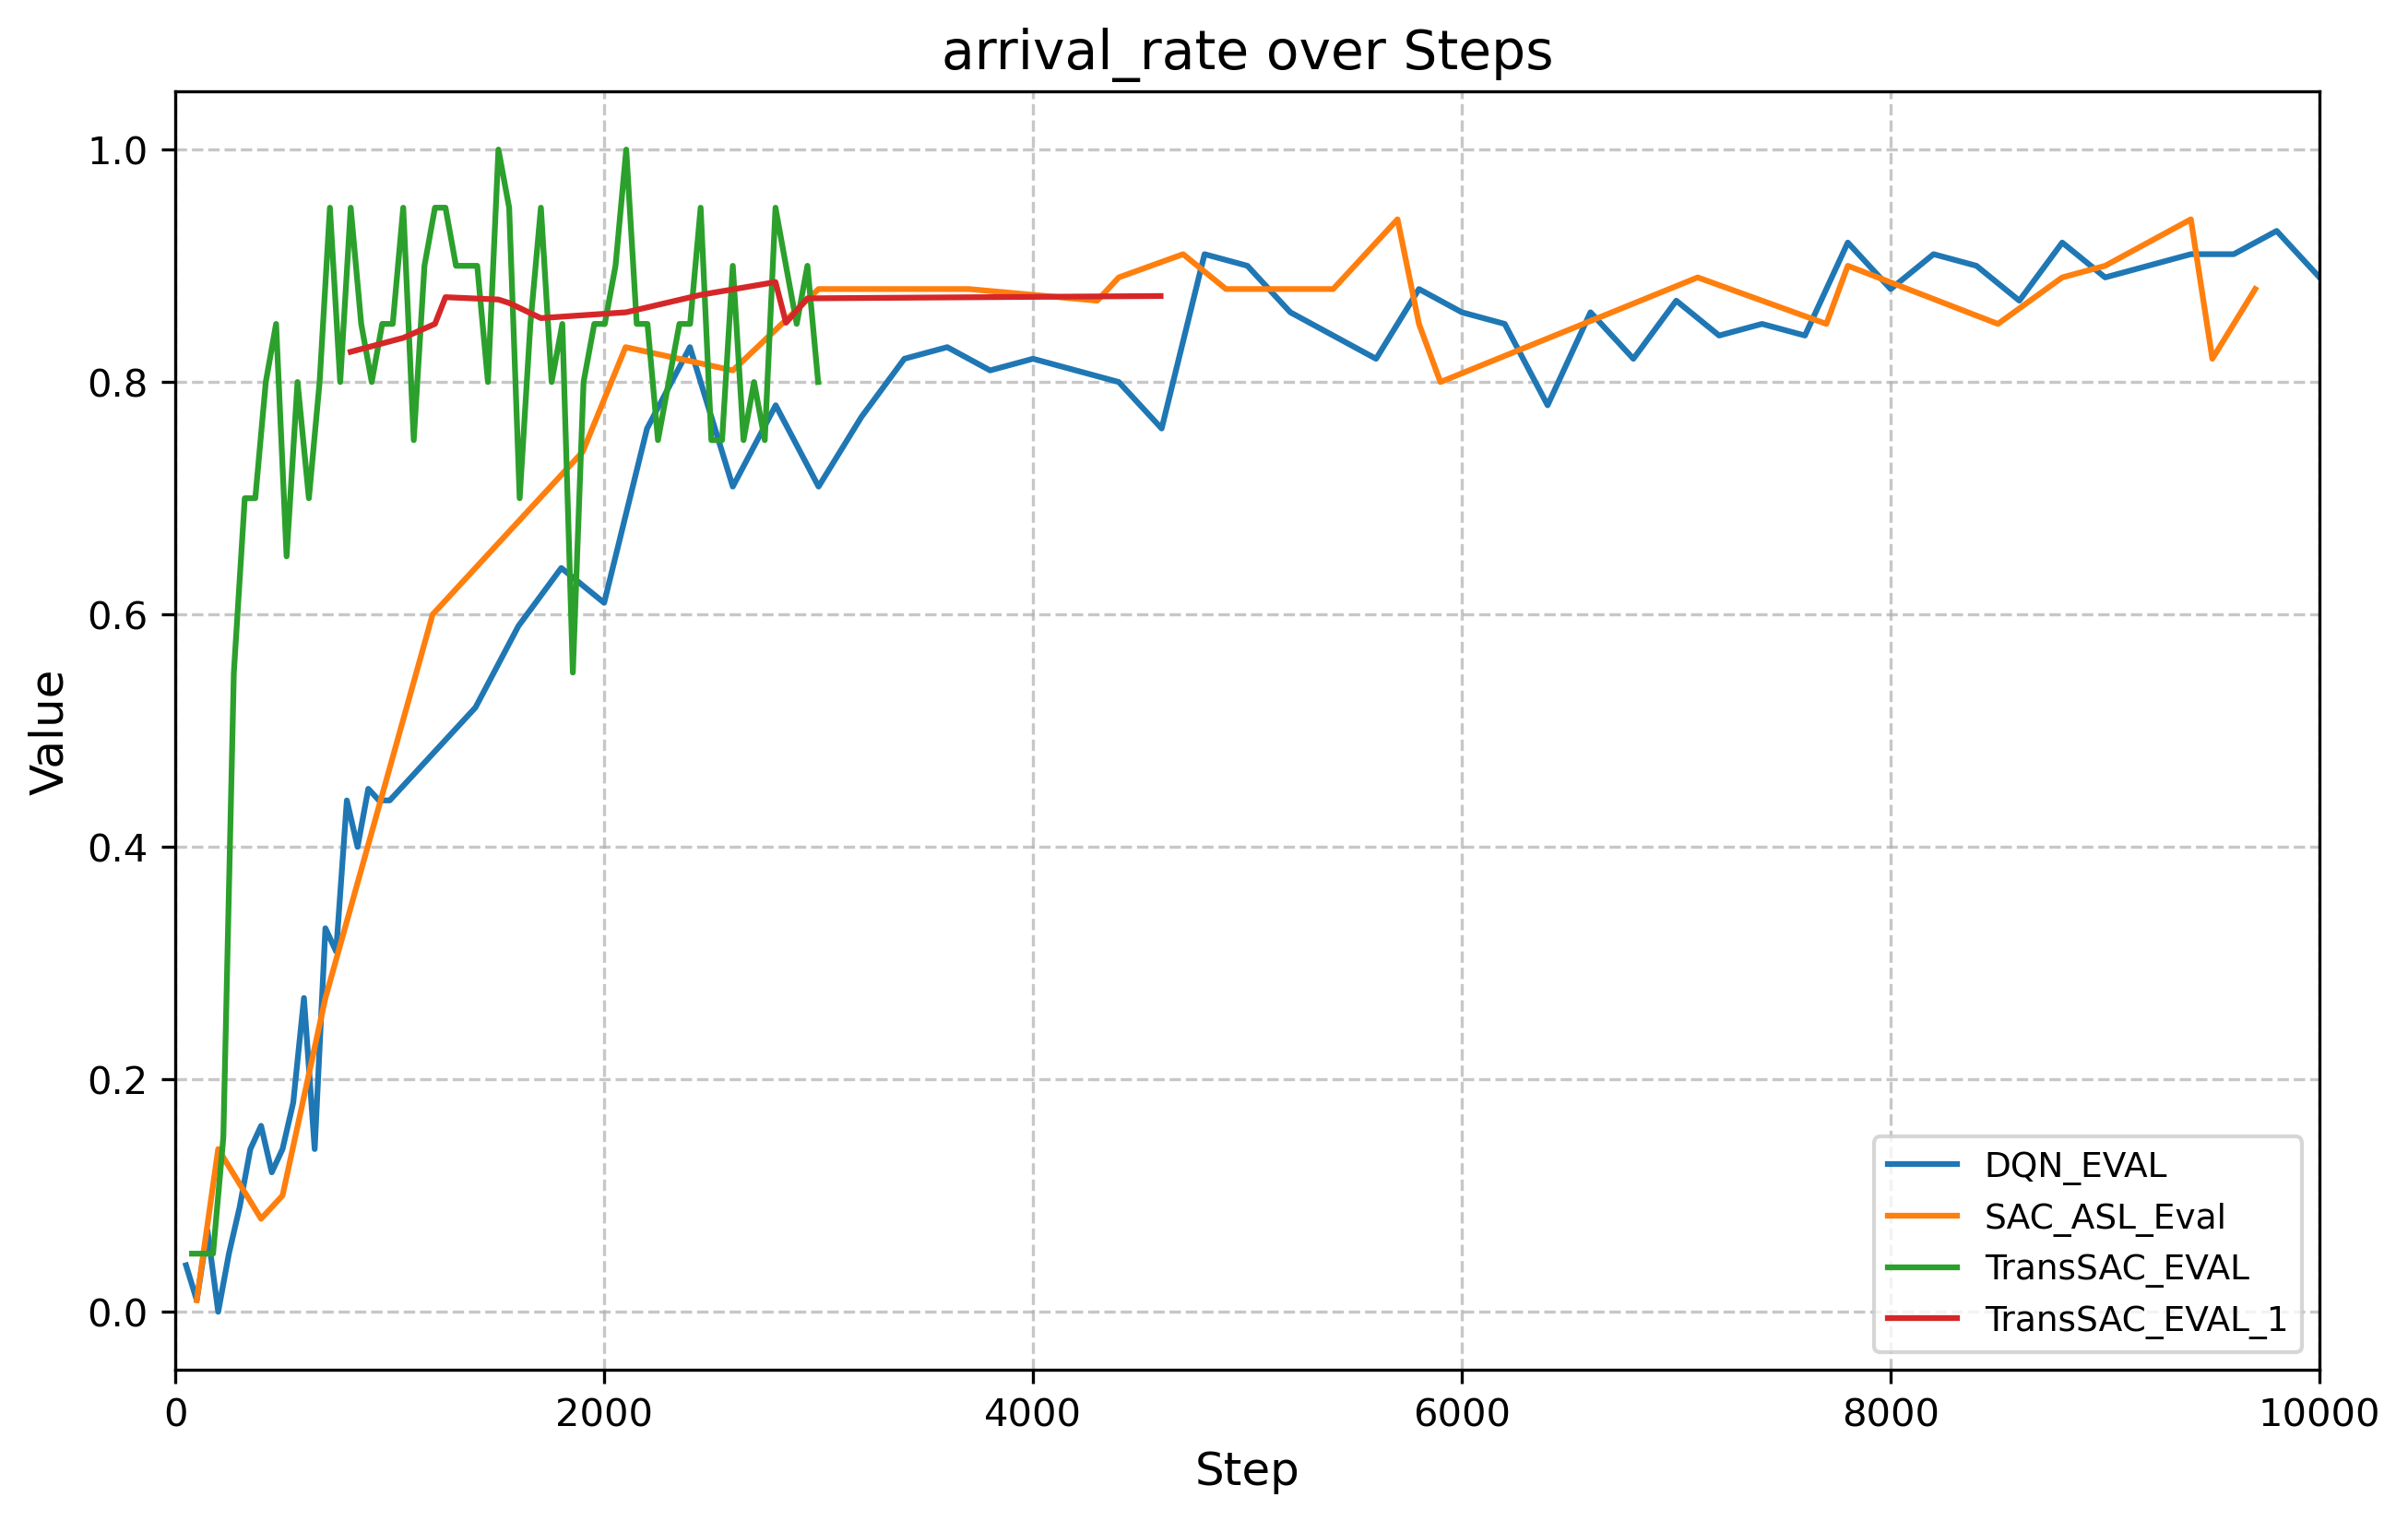
\includegraphics[width=0.7\textwidth]{figures/comparison/arrival_rate.png}
  \caption{到达率对比}
  \label{fig:comparison_arrival_rate}
\end{figure}

\begin{figure}[H]
  \centering
  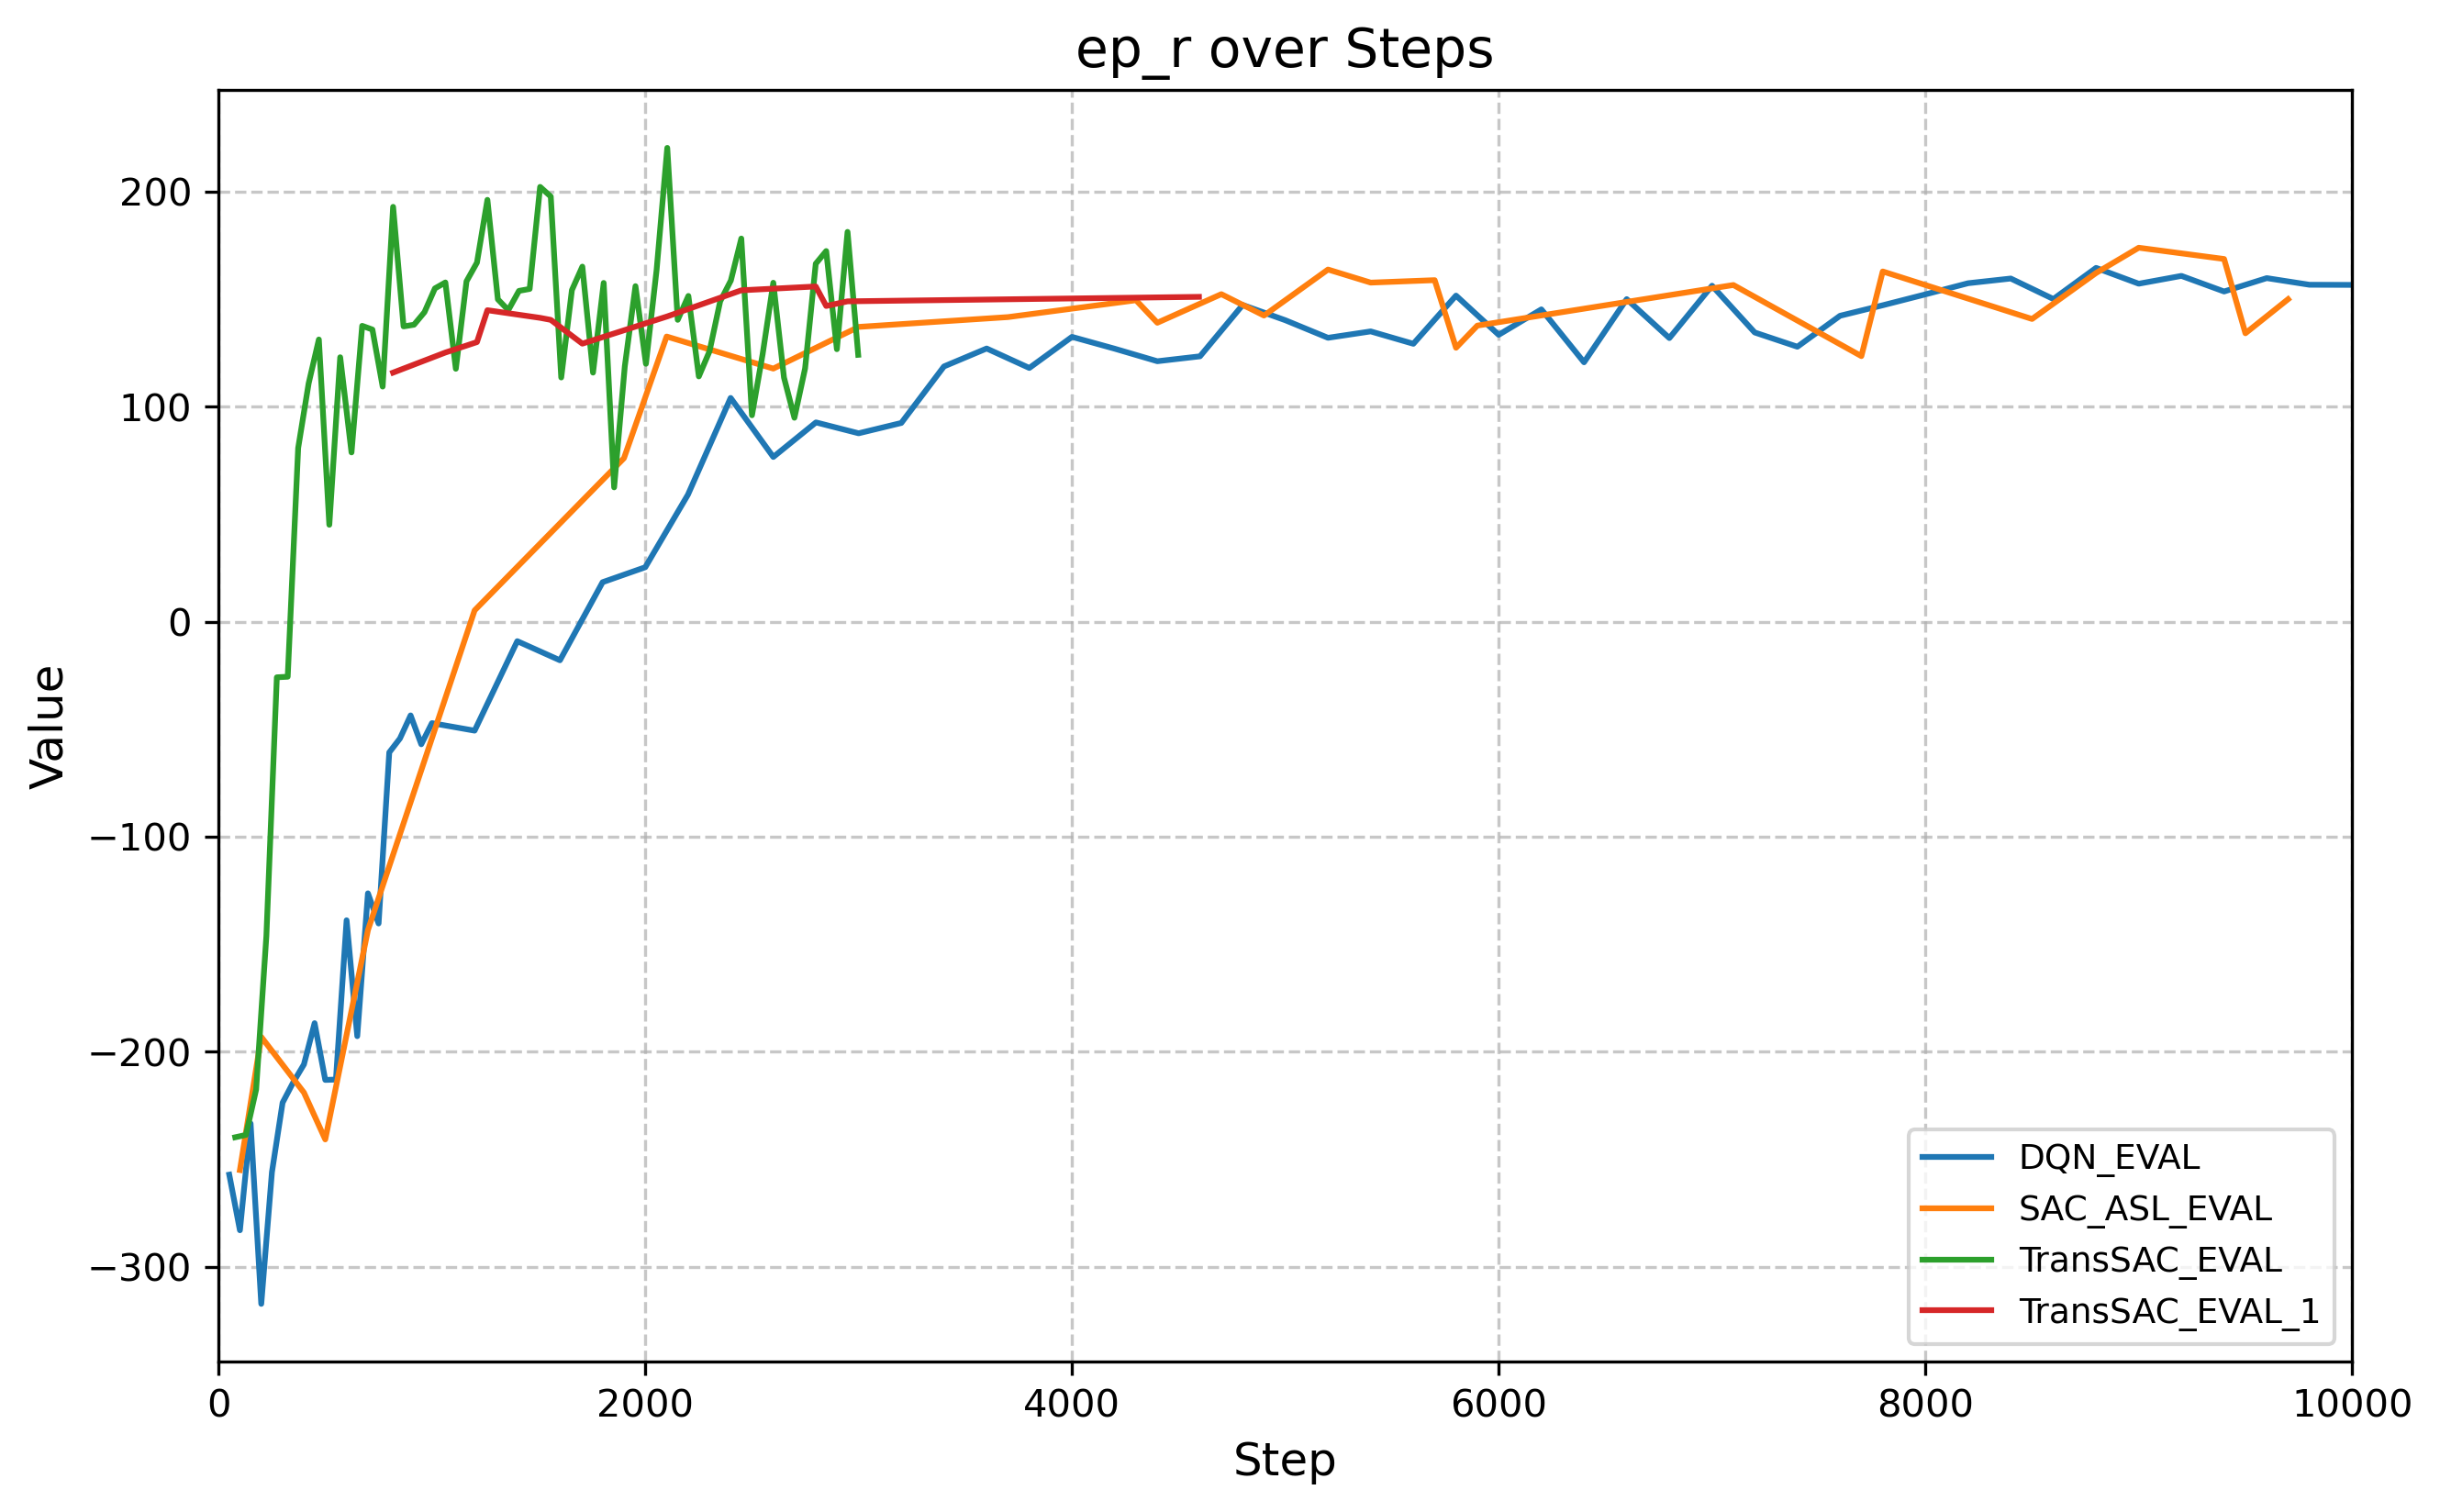
\includegraphics[width=0.7\textwidth]{figures/comparison/ep_r.png}
  \caption{累积奖励对比}
  \label{fig:comparison_ep_r}
\end{figure}

\begin{figure}[H]
  \centering
  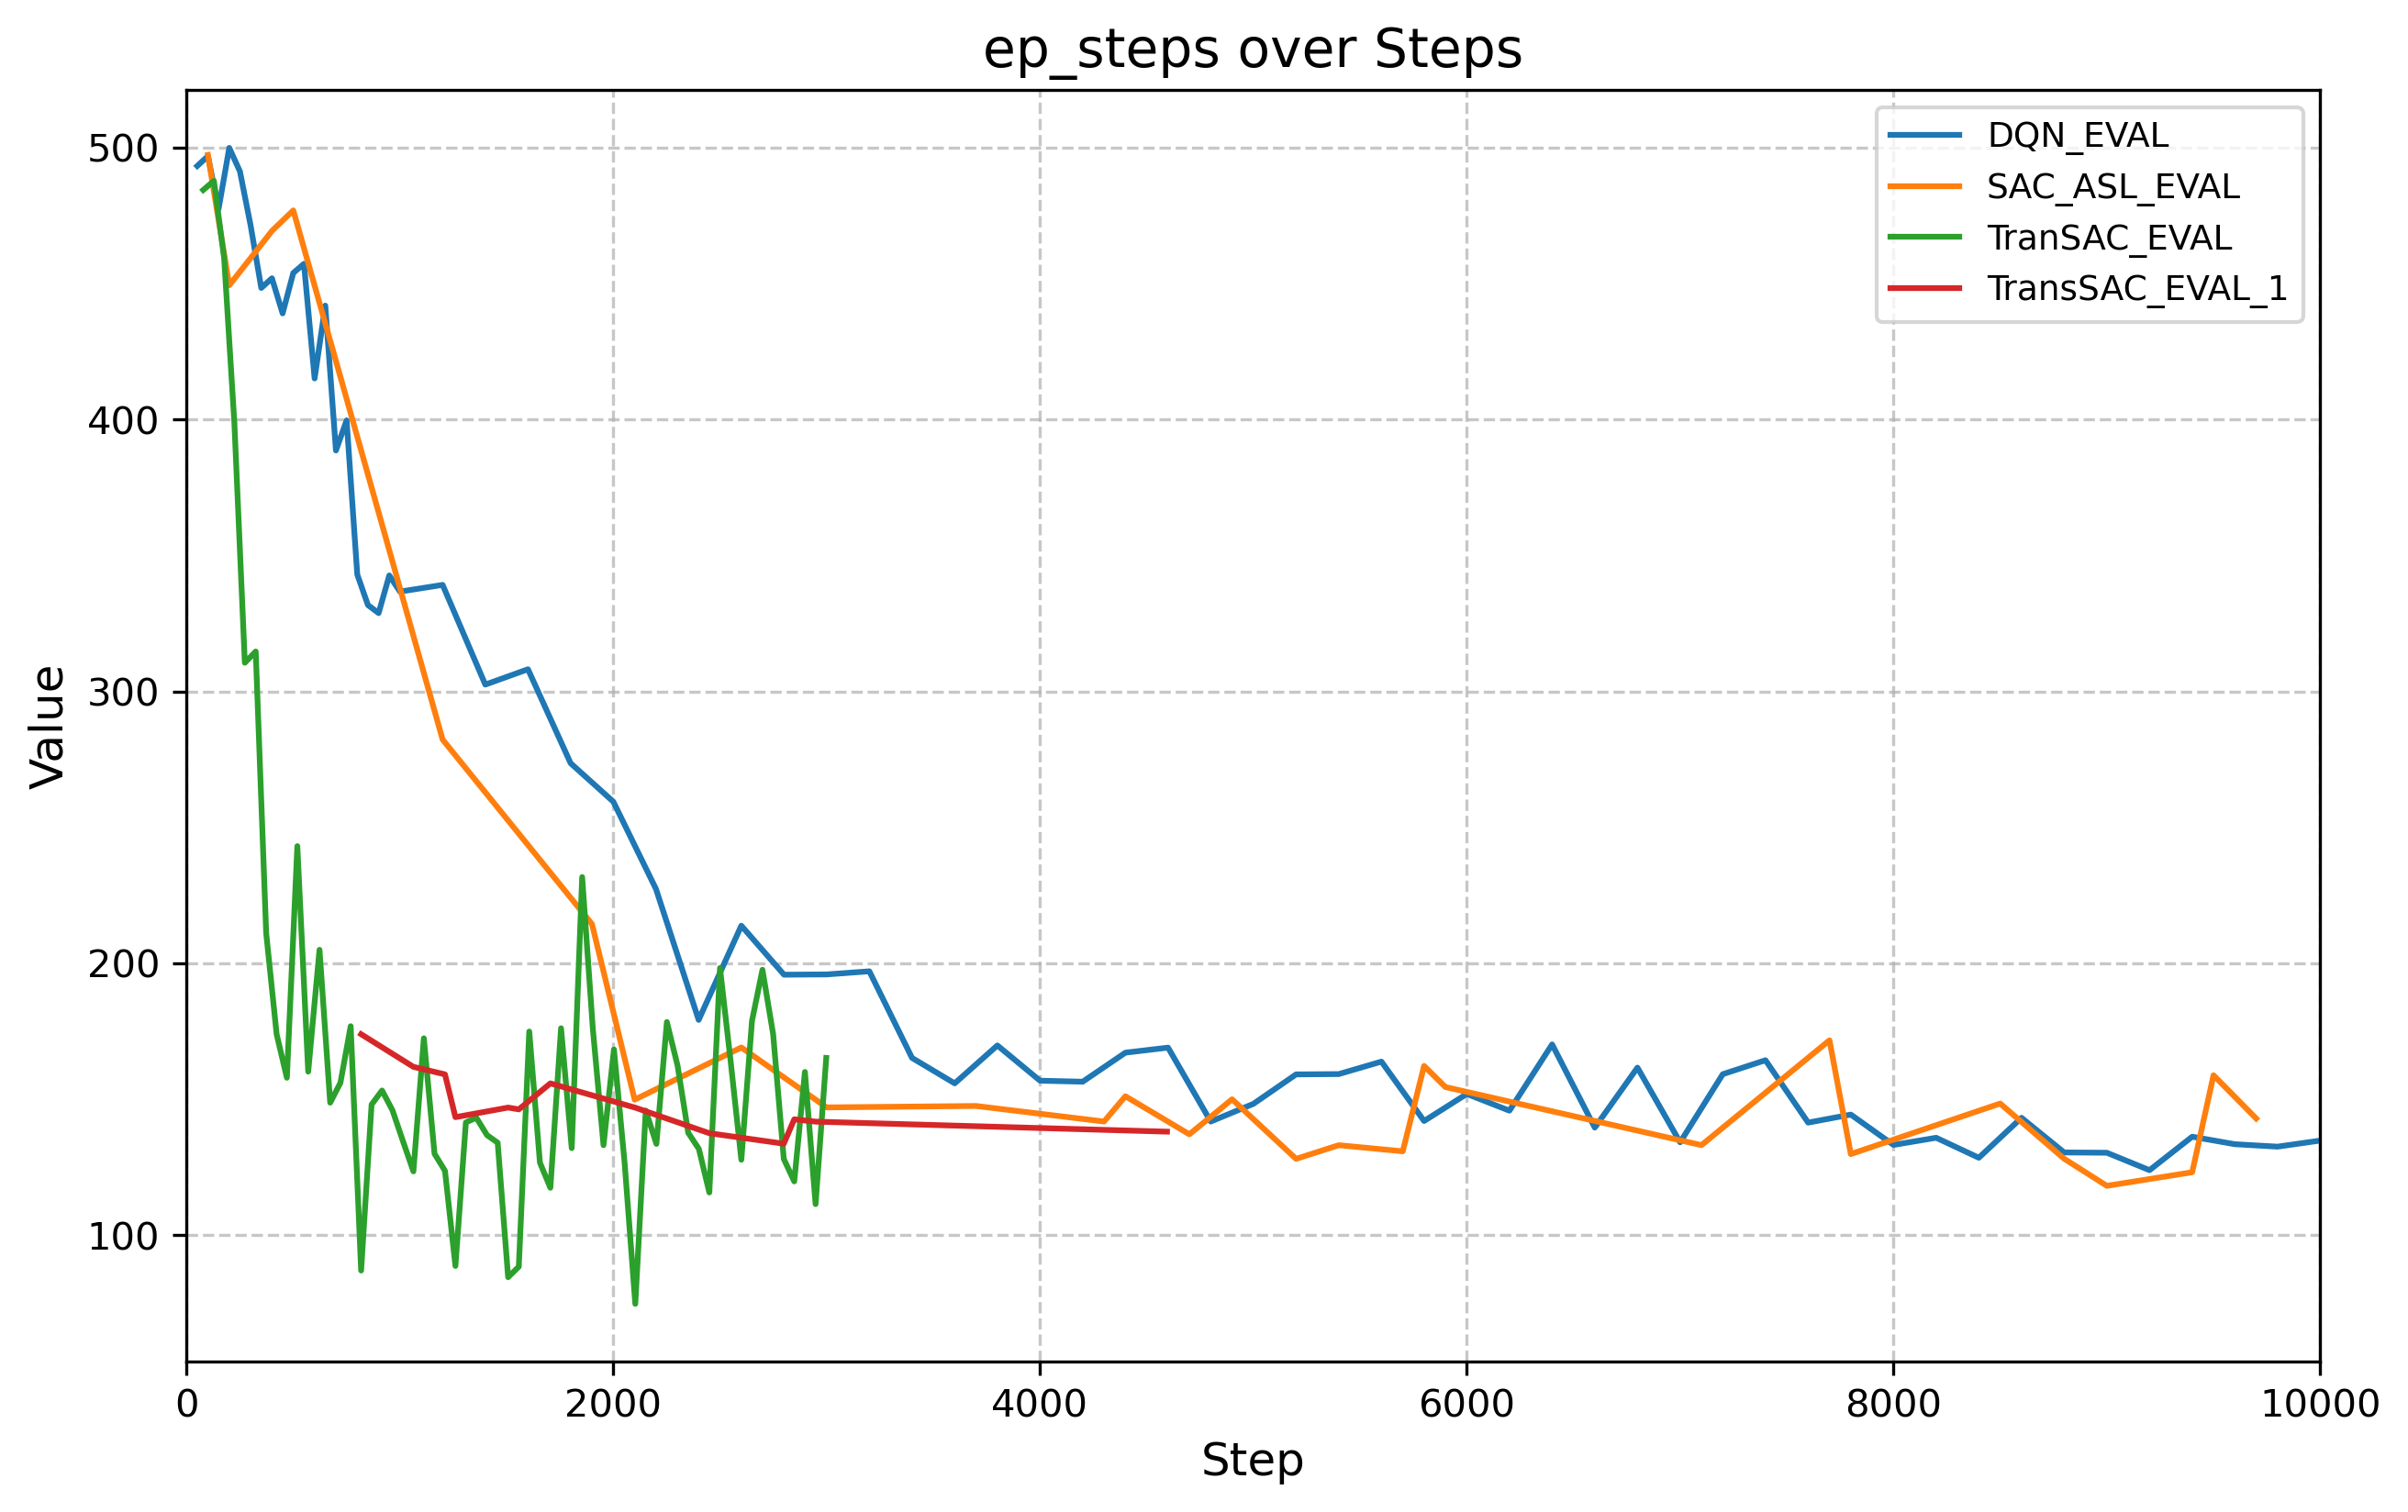
\includegraphics[width=0.7\textwidth]{figures/comparison/ep_steps.png}
  \caption{路径长度对比}
  \label{fig:comparison_ep_steps}
\end{figure}

\begin{table}[H]
    \centering
    \caption{三种路径规划算法综合性能对比}
    \label{tab:algo_comparison}
    \begin{tabular}{lcccc}
        \toprule
        \textbf{算法} & \textbf{综合评分} & \textbf{到达率} & \textbf{步数评分} & \textbf{奖励评分} \\
        \midrule
        DWA      & 0.304 & 0.530 & 0.442 & $-$0.060 \\
        DQN      & 见图~\ref{fig:dqn-showcase}     & —     & —     & — \\
        SAC      & 见图~\ref{fig:sac-showcase}     & —     & —     & — \\
        TransSAC & 见图~\ref{fig:transsac-showcase} & —     & —     & — \\
        \bottomrule
    \end{tabular}
\end{table}

\subsection{经典局部规划器与深度强化学习算法比较}

为了证明数据驱动方法在复杂动态环境下的优势，本研究首先将其与传统动态窗口法（DWA）的测试结果进行了对比。如表\ref{tab:dwa_eval_result}所总结的结果表明，经典 DWA 算法在各项导航指标上均表现出明显的局限性。具体而言，DWA 算法的到达得分（Arrival Score）仅为 0.53，这意味着在复杂的测试场景中，该算法仅有约一半的概率能够成功引导智能体到达目标点。此外，其奖励得分（Reward Score）呈现为 -0.06 的负值，且步数得分（Step Score）仅为 0.442。

对比图\ref{fig:comparison_arrival_rate}至图\ref{fig:comparison_ep_steps}中的强化学习算法收敛结果，可以发现深度强化学习模型在成功率和路径优化上实现了显著的超越。传统 DWA 算法性能低下的主要原因在于其高度依赖于人工设定的代价函数权重，且仅能在当前速度窗口内进行局部最优采样。当面对 U 型障碍物或高动态环境时，DWA 极易陷入局部极小值导致规划停滞。相反，深度强化学习算法通过在大量场景中的试错与探索，学习到了更为全局化的高级避障策略，有效克服了传统局部规划器“视野受限”的固有缺陷。

\subsection{基于深度强化学习的算法内部性能比较}

为了进一步证明引入 Transformer 架构对强化学习性能的提升，本节对 DQN、SAC 以及 TransSAC 算法在相同训练条件下的表现进行了比较。

\subsubsection{收敛速度与任务成功率：} 如图\ref{fig:comparison_arrival_rate} 的到达率（Arrival Rate）对比曲线所示，不同算法的收敛特性差异显著。TransSAC（图示绿色与红色曲线）展现出了极快的收敛速度，在经历了约 1000 个训练步（Steps）后，其到达率便迅速攀升并稳定在 0.8 以上，最终收敛于 0.9 左右的高位。相比之下，传统的 SAC\_ASL 算法（橙色曲线）虽然最终也能达到相近的成功率，但其收敛过程较为缓慢，需经历约 6000 步后方趋于稳定。而 DQN 算法（蓝色曲线）的表现最为逊色，不仅前期探索效率低下，后期也存在明显的性能震荡。TransSAC 的这一显著优势主要归功于网络结构中 Transformer 模块的引入，其强大的自注意力机制能够高效处理时序传感器数据，从而加速了智能体对环境动态的理解与策略学习。

\subsubsection{长期策略与奖励获取：} 图\ref{fig:comparison_ep_r} 展示了累积奖励（Episode Reward）随训练轮数的变化趋势。可以看出，随着训练的深入，三种算法的累积奖励均呈现上升趋势，这表明算法的奖励函数设计是合理且有效的。然而，TransSAC 模型在训练早期便能够快速脱离负奖励区间，并在后续阶段保持最高的平均累积奖励。这证实了 TransSAC 网络不仅能提高到达目标的概率，还能在规避碰撞、保持安全距离等方面做出更优的决策。

\subsubsection{路径效率与规划寻优：} 导航路径的长度是衡量规划效率的关键指标。如图\ref{fig:comparison_ep_steps} 的任务步数（Episode Steps）对比所示，在训练初期，由于处于随机探索阶段，各算法的步数均处于 400 步以上的高位。随着模型逐渐收敛，TransSAC 的步数下降最为迅速，并在 2000 步左右率先收敛至 150 步附近的极小值。DQN 算法的步数下降则最为迟缓，且后期波动较大。这一结果表明，TransSAC 由于具备更强的时间序列感知能力，能够更精准地预测动态障碍物的运动轨迹，从而为智能体规划出更加平滑、高效且接近全局最优的运动路径。

综上所述，对比实验的结果有力地证明了 TransSAC 算法在复杂导航任务中的优越性。它不仅彻底克服了经典 DWA 算法易陷入局部最优的瓶颈，而且在收敛速度、决策安全性和路径最优性方面，全面超越了传统的 DQN 与 SAC 算法。
% <<< END INPUT chapters/12_path_planning_simulation.tex
% >>> BEGIN INPUT chapters/13_conclusion.tex
\chapter{总结与展望}\label{chap:conclusion}
\section{总结}
本文以轮腿机器人的运动控制与自主导航为核心，系统性地开展了从底层控制仿真到上层路径规划算法的设计与对比研究。全文的主要工作与研究成果总结如下：

首先，在底层运动控制方面，依托Matlab构建了仿真环境。通过精细的动力学建模与参数调试，完成了轮腿机器人的姿态平衡与基础运动控制仿真验证，为上层导航与决策算法提供了可靠的物理执行器基础。

其次，在局部路径规划与自主导航方面，本文详细梳理并复现了经典的工程导航算法DWA以及主流的深度强化学习算法（DQN 与 SAC）。针对未知复杂动态环境下的连续控制难题，本文引入并验证了基于 Transformer 架构增强的 TransSAC 算法。

最后，通过搭建高效的分布式强化学习训练框架，有效提升了多环境并行采样的效率。对比实验的量化分析表明：传统的 DWA 算法在静态或简单动态环境中具备较好的可解释性与稳定性；而相比于基础的 DQN 与 SAC，本文探讨的 TransSAC 算法在部分可观测环境（POMDP）中展现出了更优的长时序特征提取能力、更高的探索效率以及面对复杂动态障碍物时更强的避障鲁棒性。
\section{展望}
本文的研究为电缆通道检测机器人的自主运动提供了较为完整的控制与规划框架，但仍存在进一步提升的空间。首先，当前控制与规划主要基于仿真环境验证，后续可结合真实样机与现场测试，对模型参数、控制律以及奖励函数进行针对性修正，以增强方法的工程适配性和鲁棒性。其次，本文的路径规划主要面向二维导航场景，未来可以进一步融合三维环境感知、语义地图与多传感器信息，使机器人对复杂电缆通道中的坡道、台阶、积水和狭窄分支具备更强的识别与决策能力。

此外，TransSAC 虽然在复杂动态环境中表现出较好的路径效率，但其训练过程对超参数和时序窗口较为敏感，后续可尝试引入更轻量的时序建模结构、自适应奖励调整机制以及更高效的分布式训练策略，以降低训练成本并提升泛化能力。随着感知、控制与智能决策技术的持续发展，电缆通道检测机器人有望在自动巡检、缺陷识别和全自主运维等方向取得更广泛的应用。
% <<< END INPUT chapters/13_conclusion.tex
% \input{chapters/14_appendix_DWA.tex}
% \input{chapters/01_guide}
% \input{chapters/02_intro}
% \input{chapters/03_float}
% \input{chapters/04_math}
% \input{chapters/05_reference}
% \input{chapters/06_conclusion}
\makereferences

\appendix
% >>> BEGIN INPUT chapters/14_appendix_control.tex
\chapter{控制器实现代码附录}\label{chap:control-code}
\subsection{控制器部分}
\begin{minted}[breaklines,linenos,fontsize=\small]{C++}

namespace controllers
{

TandemLeg::TandemLeg(
  sp::Mahony & imu, float wheel_radius, float wheel_distance, float l1, float l2, float l3,
  float l4, float lf_ecd, float lr_ecd, float rf_ecd, float rr_ecd, bool reverse_lf,
  bool reverse_lr, bool reverse_rf, bool reverse_rr, bool reverse_left_wheel,
  bool reverse_right_wheel)
: imu_(imu),
  wheel_radius_(wheel_radius),
  wheel_distance_(wheel_distance),
  l1_(l1),
  l2_(l2),
  l3_(l3),
  l4_(l4),
  lf_ecd_(lf_ecd),
  lr_ecd_(lr_ecd),
  rf_ecd_(rf_ecd),
  rr_ecd_(rr_ecd),
  reverse_lf_(reverse_lf),
  reverse_lr_(reverse_lr),
  reverse_rf_(reverse_rf),
  reverse_rr_(reverse_rr),
  reverse_left_wheel_(reverse_left_wheel),
  reverse_right_wheel_(reverse_right_wheel)
{
  this->bar.l1 = l1_;
  this->bar.l2 = l2_;
  this->bar.l3 = l3_;
  this->bar.l4 = l4_;
  this->bar.l5 = 0.0f;
}

void TandemLeg::disable() { mode_ = ControlMode::DISABLE; }

//普通力控模式
void TandemLeg::cmd_force(ChassisState & cmd)
{
  mode_ = ControlMode::FORCE;
  cmd_ = cmd;
  //关闭s项和rotate项
  cmd_.s = fdb_.s;
  cmd_.rotate = fdb_.rotate;
}

//翻倒起身速控
void TandemLeg::cmd_velocity() { mode_ = ControlMode::VELOCITY; }

//防溜车“位控”
void TandemLeg::cmd_position(ChassisState & cmd)
{
  mode_ = ControlMode::POSITION;
  cmd_ = cmd;
}

void TandemLeg::init()
{
  left_wheel_ecd_ = chassis::motor_left_wheel.angle;
  right_wheel_ecd_ = chassis::motor_right_wheel.angle;
}

void TandemLeg::control()
{
  if (mode_ == ControlMode::DISABLE) {
    chassis::motor_lr.cmd(0.0f);
    chassis::motor_lf.cmd(0.0f);
    chassis::motor_rr.cmd(0.0f);
    chassis::motor_rf.cmd(0.0f);
    chassis::motor_left_wheel.cmd(0.0f);
    chassis::motor_right_wheel.cmd(0.0f);
    return;
  }
  if (mode_ == ControlMode::VELOCITY) {
  }
  if (mode_ == ControlMode::FORCE) {
#ifdef K_FIT_ENABLED
    lqr.k_fit(tandem_leg.leg_l.l0, tandem_leg.leg_r.l0);
#endif
    tandem_leg.input = lqr.calc(cmd_, fdb_);
    tandem_leg.F0_calc();
    tandem_leg.vmc_calc();
  }
  if (mode_ == ControlMode::POSITION) {
#ifdef K_FIT_ENABLED
    lqr.k_fit(tandem_leg.leg_l.l0, tandem_leg.leg_r.l0);
#endif
    tandem_leg.input = lqr.calc(cmd_, fdb_, true);
    tandem_leg.F0_calc();
    tandem_leg.vmc_calc();
  }
  chassis::motor_lf.cmd(sp::limit_max(tandem_leg.input.t_lf, TandemLeg::MAX_HIP_TORQUE));
  chassis::motor_lr.cmd(sp::limit_max(tandem_leg.input.t_lr, TandemLeg::MAX_HIP_TORQUE));
  chassis::motor_rf.cmd(sp::limit_max(tandem_leg.input.t_rf, TandemLeg::MAX_HIP_TORQUE));
  chassis::motor_rr.cmd(sp::limit_max(tandem_leg.input.t_rr, TandemLeg::MAX_HIP_TORQUE));
  chassis::motor_left_wheel.cmd(sp::limit_max(tandem_leg.input.t_wl, TandemLeg::MAX_WHEEL_TORQUE));
  chassis::motor_right_wheel.cmd(sp::limit_max(tandem_leg.input.t_wr, TandemLeg::MAX_WHEEL_TORQUE));
  // chassis::motor_lr.cmd(0.0f);
  // chassis::motor_lf.cmd(0.0f);
  // chassis::motor_rr.cmd(0.0f);
  // chassis::motor_rf.cmd(0.0f);
  // chassis::motor_left_wheel.cmd(0.0f);
  // chassis::motor_right_wheel.cmd(0.0f);
}

void TandemLeg::update()
{
  chassis::filter_chassis();
  update_wheel(
    chassis::left_wheel_speed_filter.out, chassis::right_wheel_speed_filter.out,
    chassis::left_wheel_angle_filter.out, chassis::right_wheel_angle_filter.out, left_wheel_ecd_,
    right_wheel_ecd_);
  update_joint(
    chassis::motor_lf.angle, chassis::motor_lr.angle, chassis::motor_rf.angle,
    chassis::motor_rr.angle, chassis::lf_speed_filter.out, chassis::lr_speed_filter.out,
    chassis::rf_speed_filter.out, chassis::rr_speed_filter.out);
  update_leg(leg_l);
  update_leg(leg_r);
  update_chassis_state();
  //KF观测速度
  kf_update_z();
  ekf::kf.predict(ekf::F, ekf::Q);
  // ekf::kf.update(ekf::z, ekf::H, ekf::R);

  slip_detect();
  support_F_calc();
}

void TandemLeg::update_wheel(
  float left_wheel_speed, float right_wheel_speed, float left_wheel_angle, float right_wheel_angle,
  float left_wheel_ecd, float right_wheel_ecd)
{
  state.l_dtheta = (reverse_left_wheel_) ? -left_wheel_speed : left_wheel_speed;
  state.r_dtheta = (reverse_right_wheel_) ? -right_wheel_speed : right_wheel_speed;
  state.l_theta = (reverse_left_wheel_ ? -1.0f : 1.0f) * (left_wheel_angle - left_wheel_ecd);
  state.r_theta = (reverse_right_wheel_ ? -1.0f : 1.0f) * (right_wheel_angle - right_wheel_ecd);
}

void TandemLeg::update_joint(
  float lf_angle, float lr_angle, float rf_angle, float rr_angle, float lf_speed, float lr_speed,
  float rf_speed, float rr_speed)
{
  state.l_phi1 = sp::limit_angle((reverse_lf_ ? -1.0f : 1.0f) * (lf_angle - this->lf_ecd_));
  state.l_phi4 = sp::limit_angle((reverse_lr_ ? -1.0f : 1.0f) * (lr_angle - this->lr_ecd_));
  state.r_phi1 = sp::limit_angle((reverse_rf_ ? -1.0f : 1.0f) * (rf_angle - this->rf_ecd_));
  state.r_phi4 = sp::limit_angle((reverse_rr_ ? -1.0f : 1.0f) * (rr_angle - this->rr_ecd_));

  state.l_dphi1 = (reverse_lf_ ? -1.0f : 1.0f) * lf_speed;
  state.l_dphi4 = (reverse_lr_ ? -1.0f : 1.0f) * lr_speed;
  state.r_dphi1 = (reverse_rf_ ? -1.0f : 1.0f) * rf_speed;
  state.r_dphi4 = (reverse_rr_ ? -1.0f : 1.0f) * rr_speed;

  leg_l.phi1 = state.l_phi1;
  leg_l.phi4 = state.l_phi4;
  leg_r.phi1 = state.r_phi1;
  leg_r.phi4 = state.r_phi4;
}

void TandemLeg::update_leg(Leg & leg)
{
  const float L5 = 0.0f;

  float YD = l4_ * std::sin(leg.phi4);
  float YB = l1_ * std::sin(leg.phi1);
  float XD = L5 + l4_ * std::cos(leg.phi4);
  float XB = l1_ * std::cos(leg.phi1);

  float lBD = std::sqrt((XD - XB) * (XD - XB) + (YD - YB) * (YD - YB));
  float A0 = 2 * l2_ * (XD - XB);
  float B0 = 2 * l2_ * (YD - YB);
  float C0 = l2_ * l2_ + lBD * lBD - l3_ * l3_;

  leg.phi2 = 2 * std::atan2((B0 + std::sqrt(A0 * A0 + B0 * B0 - C0 * C0)), (A0 + C0));
  leg.phi3 = std::atan2(YB - YD + l2_ * std::sin(leg.phi2), XB - XD + l2_ * std::cos(leg.phi2));

  float XC = l1_ * std::cos(leg.phi1) + l2_ * std::cos(leg.phi2);
  float YC = l1_ * std::sin(leg.phi1) + l2_ * std::sin(leg.phi2);

  float L0 = std::sqrt((XC - L5 / 2) * (XC - L5 / 2) + YC * YC);
  float phi0 = std::atan2(YC, (XC - L5 / 2));

  leg.xc = XC;
  leg.yc = YC;
  leg.l0 = L0;
  leg.phi0 = phi0;

  leg.phi0_real = phi0 + imu_.pitch;

  leg.dphi2 = 1 / (-l2_ * sin(leg.phi2 - leg.phi3)) *
              (l1_ * sin(leg.phi1 - leg.phi3) * state.l_dphi1 -
               l4_ * sin(leg.phi4 - leg.phi3) * state.l_dphi4);
  if (&leg == &leg_l) {
    fdb_.theta_ll = leg.phi0_real - sp::Pi / 2.0f;
    fdb_.l_l0 = leg.l0;
  }
  else if (&leg == &leg_r) {
    fdb_.theta_lr = leg.phi0_real - sp::Pi / 2.0f;
    fdb_.r_l0 = leg.l0;
  }
  get_fdb_dtheta();
  get_fdb_dl0();
}

void TandemLeg::update_chassis_state()
{
  if (mode_ == ControlMode::POSITION) {
    this->fdb_.s += this->fdb_.ds * chassis::CHASSIS_CONTROL_T;
    this->fdb_.rotate += this->fdb_.drotate * chassis::CHASSIS_CONTROL_T;
  }
  else {
    this->fdb_.s = 0.0f;
    this->fdb_.rotate = 0.0f;
  }
  this->fdb_.ds = this->wheel_radius_ / 2.0f * (this->state.l_dtheta + this->state.r_dtheta);
  this->fdb_.drotate =
    this->wheel_radius_ / 2.0f / this->wheel_distance_ *
      (this->state.r_dtheta - this->state.l_dtheta) -
    leg_l.l0 / 2.0f / this->wheel_distance_ * cos(fdb_.theta_ll) * fdb_.dtheta_ll +
    leg_r.l0 / 2.0f / this->wheel_distance_ * cos(fdb_.theta_lr) * fdb_.dtheta_lr;
  this->fdb_.phi = imu_.pitch;
  this->fdb_.dphi = imu_.vpitch;
}

void TandemLeg::vmc_calc()
{
  //左腿
  float l_j11 = (bar.l1 * sin(leg_l.phi0 - leg_l.phi3) * sin(leg_l.phi1 - leg_l.phi2)) /
                sin(leg_l.phi3 - leg_l.phi2);
  float l_j12 = (bar.l1 * cos(leg_l.phi0 - leg_l.phi3) * sin(leg_l.phi1 - leg_l.phi2)) /
                (leg_l.l0 * sin(leg_l.phi3 - leg_l.phi2));
  float l_j21 = (bar.l4 * sin(leg_l.phi0 - leg_l.phi2) * sin(leg_l.phi3 - leg_l.phi4)) /
                sin(leg_l.phi3 - leg_l.phi2);
  float l_j22 = (bar.l4 * cos(leg_l.phi0 - leg_l.phi2) * sin(leg_l.phi3 - leg_l.phi4)) /
                (leg_l.l0 * sin(leg_l.phi3 - leg_l.phi2));

  input.t_lf = (reverse_lf_ ? -1.0f : 1.0f) * (l_j11 * input.f0_l + l_j12 * input.tp_l);
  input.t_lr = (reverse_lr_ ? -1.0f : 1.0f) * (l_j21 * input.f0_l + l_j22 * input.tp_l);
  input.t_wl = (reverse_left_wheel_ ? -1.0f : 1.0f) * input.t_wl;  //左轮

  //右腿
  float r_j11 = (bar.l1 * sin(leg_r.phi0 - leg_r.phi3) * sin(leg_r.phi1 - leg_r.phi2)) /
                sin(leg_r.phi3 - leg_r.phi2);
  float r_j12 = (bar.l1 * cos(leg_r.phi0 - leg_r.phi3) * sin(leg_r.phi1 - leg_r.phi2)) /
                (leg_r.l0 * sin(leg_r.phi3 - leg_r.phi2));
  float r_j21 = (bar.l4 * sin(leg_r.phi0 - leg_r.phi2) * sin(leg_r.phi3 - leg_r.phi4)) /
                sin(leg_r.phi3 - leg_r.phi2);
  float r_j22 = (bar.l4 * cos(leg_r.phi0 - leg_r.phi2) * sin(leg_r.phi3 - leg_r.phi4)) /
                (leg_r.l0 * sin(leg_r.phi3 - leg_r.phi2));

  input.t_rf = (reverse_rf_ ? -1.0f : 1.0f) * (r_j11 * input.f0_r + r_j12 * input.tp_r);
  input.t_rr = (reverse_rr_ ? -1.0f : 1.0f) * (r_j21 * input.f0_r + r_j22 * input.tp_r);
  input.t_wr = (reverse_right_wheel_ ? -1.0f : 1.0f) * input.t_wr;  //右轮
}

void TandemLeg::F0_calc()
{
  //支持力=重力补偿+腿长补偿+roll补偿+侧向惯性力矩补偿
  float chassis_force = chassis::CHASSIS_WEIGHT * chassis::GRAVITY_ACC;
  //重力补偿
  float F0_L = chassis_force * cosf(fdb_.theta_ll) / 2.0f;
  float F0_R = chassis_force * cosf(fdb_.theta_lr) / 2.0f;
  //腿长补偿
  l_leg_length_pid.calc(cmd_.l_l0, leg_l.l0);
  r_leg_length_pid.calc(cmd_.l_l0, leg_r.l0);
  //roll补偿
  leg_roll_pid.calc(0.0f, imu_.roll);
  //侧向惯性力矩补偿
  float lateral_inertia_torque =
    chassis::CHASSIS_WEIGHT / 2 * 1 / (2 * chassis::WHEEL_DISTANCE) * fdb_.dphi * fdb_.s;
  input.f0_l = F0_L + l_leg_length_pid.out + leg_roll_pid.out - lateral_inertia_torque;
  input.f0_r = F0_R + r_leg_length_pid.out - leg_roll_pid.out + lateral_inertia_torque;
}

void TandemLeg::get_fdb_dtheta()
{
  get_fdb_dtheta_leg(leg_l);
  get_fdb_dtheta_leg(leg_r);
}

void TandemLeg::get_fdb_dtheta_leg(Leg & leg)
{
  float J11 = bar.l1 * sin(leg.phi1 - leg.phi2) * sin(leg.phi3) / sin(leg.phi2 - leg.phi3);
  float J12 = bar.l4 * sin(leg.phi3 - leg.phi4) * sin(leg.phi2) / sin(leg.phi2 - leg.phi3);
  float J21 = -bar.l1 * sin(leg.phi1 - leg.phi2) * sin(leg.phi3) / sin(leg.phi2 - leg.phi3);
  float J22 = -bar.l4 * sin(leg.phi3 - leg.phi4) * sin(leg.phi2) / sin(leg.phi2 - leg.phi3);

  if (&leg == &leg_l) {
    float dxc_l = J11 * state.l_dphi1 + J12 * state.l_dphi4;
    float dyc_l = J21 * state.l_dphi1 + J22 * state.l_dphi4;
    fdb_.dtheta_ll =
      -(leg.yc * dxc_l - leg.xc * dyc_l) / (leg.xc * leg.xc + leg.yc * leg.yc) + imu.vpitch;
  }
  if (&leg == &leg_r) {
    float dxc_l = J11 * state.r_dphi1 + J12 * state.r_dphi4;
    float dyc_l = J21 * state.r_dphi1 + J22 * state.r_dphi4;
    fdb_.dtheta_lr =
      -(leg.yc * dxc_l - leg.xc * dyc_l) / (leg.xc * leg.xc + leg.yc * leg.yc) + imu.vpitch;
  }
}

void TandemLeg::get_fdb_dl0()
{
  get_fdb_dl0_leg(leg_l);
  get_fdb_dl0_leg(leg_r);
}

void TandemLeg::get_fdb_dl0_leg(Leg & leg)
{
  if (&leg == &leg_l) {
    float dXC = -bar.l1 * sin(leg.phi1) * state.l_dphi1 - bar.l2 * sin(leg.phi2) * leg_l.dphi2;
    float dYC = bar.l1 * cos(leg.phi1) * state.l_dphi1 + bar.l2 * cos(leg.phi2) * leg_l.dphi2;
    fdb_.dl_l0 = (leg.xc * dXC + leg.yc * dYC) / leg.l0;
  }
  if (&leg == &leg_r) {
    float dXC = -bar.l1 * sin(leg.phi1) * state.r_dphi1 - bar.l2 * sin(leg.phi2) * leg_r.dphi2;
    float dYC = bar.l1 * cos(leg.phi1) * state.r_dphi1 + bar.l2 * cos(leg.phi2) * leg_r.dphi2;
    fdb_.dr_l0 = (leg.xc * dXC + leg.yc * dYC) / leg.l0;
  }
}

//KF更新
//需要在imu已经跑起来后调用
void TandemLeg::kf_update_z()
{
  static float last_gyro_z = imu_.vyaw;
  float acc_z = (imu_.vyaw - last_gyro_z) / CONTROL_T;

  ekf::z[0][0] = fdb_.ds;
  ekf::z[1][0] = bmi088.acc[0] * cosf(imu.pitch) - chassis::GRAVITY_ACC * sinf(imu.pitch);
  ekf::z[2][0] = fdb_.drotate;
  ekf::z[3][0] = acc_z;
  if (remote.sw_l == sp::DBusSwitchMode::DOWN) {
    ekf::kf_initialized = false;
  }
  if (!ekf::kf_initialized) {
    ekf::kf_initialized = true;
    ekf::kf.x[0][0] = ekf::z[0][0];
    ekf::kf.x[1][0] = ekf::z[1][0];
    ekf::kf.x[2][0] = ekf::z[2][0];
    ekf::kf.x[3][0] = ekf::z[3][0];
    return;
  }
}

void TandemLeg::slip_detect()
{
  // float innovation_v = chassis.fdb.ds - (z[1][0] * T_CONTROL +);  // 残差

  // 核心逻辑：如果残差过大，说明编码器速度突变（打滑），
  // 此时我们不信任编码器，极大幅度增加测量噪声 R
  if (std::abs(ekf::kf.data["ds"]) > SLIP_THRESHOLD) {
    // 检测到打滑
    // 策略：瞬间增大测量噪声，让滤波器主要保留预测值（即保留 IMU 积分结果）
    ekf::R = ekf::R_slip_data;
    slip_flag_ = true;
    // Q = q_slip_diag_vec;
    ekf::Q = ekf::Q_data_slip;
    ekf::Q[0][0] = 0.1f;
    ekf::Q[1][1] = 10.0f;
    ekf::Q[2][2] = 0.5f;
    ekf::Q[3][3] = 0.5f;
  }
  // else {
  //   R = R_data;
  //   slip_flag_ = false;
  // }
  //在0附近时来回切？
  // if(std::abs(innovation_v) <= SLIP_OVER_THRESHOLD) {
  //     // 正常情况，恢复正常测量噪声
  //     R = R_data;
  // }
}

void TandemLeg::support_F_calc()
{
  support_F_calc_leg(leg_l);
  support_F_calc_leg(leg_r);
}

void TandemLeg::support_F_calc_leg(Leg & leg)
{
  float zM = ins_accel_corrected[2];
  if (&leg == &leg_l) {
    float P = input.f0_l * cosf(state.l_theta) + input.tp_l * sinf(state.l_theta) / leg.l0;
    state.l_F0 = P + chassis::CHASSIS_WEIGHT * chassis::GRAVITY_ACC / 2.0f +
                 chassis::CHASSIS_WEIGHT * zM / 2.0f;
  }
  if (&leg == &leg_r) {
    float P = input.f0_r * cosf(state.r_theta) + input.tp_r * sinf(state.r_theta) / leg.l0;
    state.r_F0 = P + chassis::CHASSIS_WEIGHT * chassis::GRAVITY_ACC / 2.0f +
                 chassis::CHASSIS_WEIGHT * zM / 2.0f;
  }
}
}  // namespace controllers


\end{minted}

\subsection{交互部分}
\begin{minted}[breaklines,linenos,fontsize=\small]{python}
import math

import matplotlib.pyplot as plt
import numpy as np

show_animation = True  # 动画


class Config(object):
    """
    用来仿真的参数，
    """

    def __init__(self):
        # robot parameter
        self.max_speed = 0.5  # [m/s]  # 最大速度
        self.min_speed = -0.5  # [m/s]  # 最小速度，设置为可以倒车
        # self.min_speed = 0  # [m/s]  # 最小速度，设置为不倒车
        self.max_yawrate = 2  # [rad/s]  # 最大角速度
        self.max_accel = 0.2  # [m/ss]  # 最大加速度
        self.max_dyawrate = 2  # [rad/ss]  # 最大角加速度
        self.v_reso = 0.01  # [m/s]，速度分辨率
        self.yawrate_reso = 0.1  # [rad/s]，角速度分辨率
        self.dt = 0.1  # [s]  # 采样周期
        self.predict_time = 3.0  # [s]  # 向前预估三秒
        self.to_goal_cost_gain = 1.0  # 目标代价增益
        self.speed_cost_gain = 1.0  # 速度代价增益
        self.robot_radius = 0.09  # [m]  # 机器人半径

def motion(x, u, dt):
    """
    :param x: 位置参数，在此叫做位置空间
    :param u: 速度和加速度，在此叫做速度空间
    :param dt: 采样时间
    :return:
    """
    x[0] += u[0] * math.cos(x[2]) * dt  # x方向位移
    x[1] += u[0] * math.sin(x[2]) * dt  # y方向位移
    x[2] += u[1] * dt  # 航向角
    x[3] = u[0]  # 速度v
    x[4] = u[1]  # 角速度w
    return x


def calc_dynamic_window(x, config):
    """
    位置空间集合
    :param x:当前位置空间,符号参考硕士论文
    :param config:
    :return:目前是两个速度的交集，还差一个
    """

    # 车辆能够达到的最大最小速度
    vs = [config.min_speed, config.max_speed, -config.max_yawrate, config.max_yawrate]

    # 一个采样周期能够变化的最大最小速度
    vd = [
        x[3] - config.max_accel * config.dt,
        x[3] + config.max_accel * config.dt,
        x[4] - config.max_dyawrate * config.dt,
        x[4] + config.max_dyawrate * config.dt,
    ]
    #  print(Vs, Vd)

    # 求出两个速度集合的交集
    vr = [max(vs[0], vd[0]), min(vs[1], vd[1]), max(vs[2], vd[2]), min(vs[3], vd[3])]

    return vr


# 产生运动轨迹
def calc_trajectory(x_init, v, w, config):
    """
    预测3秒内的轨迹
    :param x_init:位置空间
    :param v:速度
    :param w:角速度
    :param config:
    :return: 每一次采样更新的轨迹，位置空间垂直堆叠
    """
    x = np.array(x_init)
    trajectory = np.array(x)
    time = 0
    while time <= config.predict_time:
        x = motion(x, [v, w], config.dt)
        trajectory = np.vstack((trajectory, x))  # 垂直堆叠，vertical
        time += config.dt
    return trajectory


def calc_to_goal_cost(trajectory, goal, config):
    """
    计算轨迹到目标点的代价
    :param trajectory:轨迹搜索空间
    :param goal:
    :param config:
    :return: 轨迹到目标点欧式距离
    """
    # calc to goal cost. It is 2D norm.

    dx = goal[0] - trajectory[-1, 0]
    dy = goal[1] - trajectory[-1, 1]
    goal_dis = math.sqrt(dx**2 + dy**2)
    cost = config.to_goal_cost_gain * goal_dis

    return cost


def calc_obstacle_cost(traj, ob, config):
    """
    计算预测轨迹和障碍物的最小距离，dist(v,w)
    :param traj:
    :param ob:
    :param config:
    :return:
    """
    # calc obstacle cost inf: collision, 0:free

    min_r = float("inf")  # 距离初始化为无穷大

    for ii in range(0, len(traj[:, 1])):
        for i in range(len(ob[:, 0])):
            ox = ob[i, 0]
            oy = ob[i, 1]
            dx = traj[ii, 0] - ox
            dy = traj[ii, 1] - oy

            r = math.sqrt(dx**2 + dy**2)
            if r <= config.robot_radius:
                return float("Inf")  # collision

            if min_r >= r:
                min_r = r

    return 1.0 / min_r  # 越小越好 与障碍物距离越近，该值会越大；


def calc_final_input(x, u, vr, config, goal, ob):
    """
    计算采样空间的评价函数，选择最合适的那一个作为最终输入
    :param x:位置空间
    :param u:速度空间
    :param vr:速度空间交集
    :param config:
    :param goal:目标位置
    :param ob:障碍物
    :return:
    """
    x_init = x[:]
    min_cost = 10000.0
    min_u = u

    best_trajectory = np.array([x])
    for v in np.arange(vr[0], vr[1], config.v_reso):  
        for w in np.arange(vr[2], vr[3], config.yawrate_reso): 
            trajectory = calc_trajectory(x_init, v, w, config)

            # calc cost
            to_goal_cost = calc_to_goal_cost(
                trajectory, goal, config
            )  # trajectory与目标的欧式距离
            speed_cost = config.speed_cost_gain * (
                config.max_speed - trajectory[-1, 3]
            )  # v越大，该项越小，则效果越好；
            ob_cost = calc_obstacle_cost(
                trajectory, ob, config
            )  # 返回的是距离的倒数，该值约小，距离越大，越好
            final_cost = (
                to_goal_cost + speed_cost + 0 * ob_cost
            )  # 总计代价，越小轨迹约好

            # search minimum trajectory
            if min_cost >= final_cost:
                min_cost = final_cost
                min_u = [v, w]  
                best_trajectory = trajectory  

    return min_u, best_trajectory


def dwa_control(x, u, config, goal, ob):
    """
    调用前面的几个函数，生成最合适的速度空间和轨迹搜索空间
    :param x: 起始位置
    :param u:初始速度空间（v,w）
    :param config:
    :param goal:目标位置
    :param ob:障碍物
    :return:
    """
    # Dynamic Window control

    vr = calc_dynamic_window(x, config)  # 计算动态窗口，即机器人的电机实际物理参数范围

    u, trajectory = calc_final_input(
        x, u, vr, config, goal, ob
    )  # 选出最优轨迹搜索空间和速度空间

    return u, trajectory


def plot_arrow(x, y, yaw, length=0.5, width=0.1):
    plt.arrow(
        x,
        y,
        length * math.cos(yaw),
        length * math.sin(yaw),
        head_length=1.5 * width,
        head_width=width,
    )
    plt.plot(x, y)


def main():
    x = np.array([0.0, 0.0, math.pi / 2.0, 0.2, 0.0])

    goal = np.array([10, 10])

    # matrix二维矩阵 障碍物
    ob = np.matrix(
        [
            [-1, -1],
            [0, 2],
            [4.0, 2.0],
            [5.0, 4.0],
            [5.0, 5.0],
            [5.0, 6.0],
            [5.0, 9.0],
            [8.0, 9.0],
            [7.0, 9.0],
            [12.0, 12.0],
        ]
    )
    # ob = np.matrix([[0, 2]])
    # ob = np.matrix([[2, 2]])

    u = np.array([0.2, 0.0])  # 初始速度空间(v,w)
    config = Config()  # 初始化物理运动参数
    trajectory = np.array(x)  # 初始轨迹空间

    for i in range(1000):
        u, best_trajectory = dwa_control(
            x, u, config, goal, ob
        )  # 获取最优速度空间和轨迹参数
        x = motion(x, u, config.dt)  # 机器人运动方程 x为机器人状态空间

        trajectory = np.vstack((trajectory, x))  # store state history

        if show_animation:
            draw_dynamic_search(best_trajectory, x, goal, ob)

        # check goal
        if (
            math.sqrt((x[0] - goal[0]) ** 2 + (x[1] - goal[1]) ** 2)
            <= config.robot_radius
        ):
            print("Goal!!")
            break

    print("Done")

    draw_path(trajectory, goal, ob, x)


def draw_dynamic_search(best_trajectory, x, goal, ob):
    """
    画出动态搜索过程图
    :return:
    """
    plt.cla()  # 清除上次绘制图像
    plt.plot(best_trajectory[:, 0], best_trajectory[:, 1], "-g")
    plt.plot(x[0], x[1], "xr")
    plt.plot(0, 0, "og")
    plt.plot(goal[0], goal[1], "ro")
    plt.plot(ob[:, 0], ob[:, 1], "bs")
    plot_arrow(x[0], x[1], x[2])
    plt.axis("equal")
    plt.grid(True)
    plt.pause(0.0001)


def draw_path(trajectory, goal, ob, x):
    """
    画图函数
    :return:
    """
    plt.cla()  # 清除上次绘制图像

    plt.plot(x[0], x[1], "xr")
    plt.plot(0, 0, "og")
    plt.plot(goal[0], goal[1], "ro")
    plt.plot(ob[:, 0], ob[:, 1], "bs")
    plot_arrow(x[0], x[1], x[2])
    plt.axis("equal")
    plt.grid(True)
    plt.plot(trajectory[:, 0], trajectory[:, 1], "r")
    plt.show()


if __name__ == "__main__":
    main()
\end{minted}
% <<< END INPUT chapters/14_appendix_control.tex

\backmatter
% >>> BEGIN INPUT chapters/ack.tex
\chapter*{谢\hspace{0.5em}辞}
\addcontentsline{toc}{chapter}{谢\hspace{0.5em}辞}

感谢指导老师的悉心指导和耐心帮助，使我在毕业设计过程中能够顺利完成研究工作。老师在选题到具体算法参数调优上都给予了我许多宝贵的建议。

感谢SuperPower战队，为我提供了工位以及测试设备。本科期间在战队里学习了机器人学相关知识、积累了机器人实机调试经验，这些都为我的毕业设计提供了坚实的基础。同时，战队的同学们不仅在相关专业知识上给予了我很多帮助，他们严谨务实的态度也深深影响了我，让我在毕业设计过程中能够保持专注和耐心。

感谢我的家人，在我求学的道路上给予了我无私的支持和鼓励。无论是在学业上还是生活中，他们一直是我坚强的后盾，让我能够专注于学业，顺利完成毕业设计。

最后感谢我自己，这一年来在各个方面都成长许多。这几年来我对于个人的职业追求一直是成为一个快乐的工程师，在纯粹的技术追求中感受快乐，在生活的点点滴滴中感受微小的幸福。很惭愧大学生活的前几年总会纠结于各种小事；但过去的半年我想我确实是快乐且纯粹的，而且相信明年的我将更加成熟和幸福。
% <<< END INPUT chapters/ack.tex

\end{document}
